% Options for packages loaded elsewhere
\PassOptionsToPackage{unicode}{hyperref}
\PassOptionsToPackage{hyphens}{url}
\PassOptionsToPackage{dvipsnames,svgnames,x11names}{xcolor}
%
\documentclass[
  letterpaper,
  DIV=11,
  numbers=noendperiod,
  oneside]{scrreprt}

\usepackage{amsmath,amssymb}
\usepackage{iftex}
\ifPDFTeX
  \usepackage[T1]{fontenc}
  \usepackage[utf8]{inputenc}
  \usepackage{textcomp} % provide euro and other symbols
\else % if luatex or xetex
  \usepackage{unicode-math}
  \defaultfontfeatures{Scale=MatchLowercase}
  \defaultfontfeatures[\rmfamily]{Ligatures=TeX,Scale=1}
\fi
\usepackage{lmodern}
\ifPDFTeX\else  
    % xetex/luatex font selection
\fi
% Use upquote if available, for straight quotes in verbatim environments
\IfFileExists{upquote.sty}{\usepackage{upquote}}{}
\IfFileExists{microtype.sty}{% use microtype if available
  \usepackage[]{microtype}
  \UseMicrotypeSet[protrusion]{basicmath} % disable protrusion for tt fonts
}{}
\makeatletter
\@ifundefined{KOMAClassName}{% if non-KOMA class
  \IfFileExists{parskip.sty}{%
    \usepackage{parskip}
  }{% else
    \setlength{\parindent}{0pt}
    \setlength{\parskip}{6pt plus 2pt minus 1pt}}
}{% if KOMA class
  \KOMAoptions{parskip=half}}
\makeatother
\usepackage{xcolor}
\usepackage[left=1in,marginparwidth=2.0666666666667in,textwidth=4.1333333333333in,marginparsep=0.3in]{geometry}
\setlength{\emergencystretch}{3em} % prevent overfull lines
\setcounter{secnumdepth}{5}
% Make \paragraph and \subparagraph free-standing
\ifx\paragraph\undefined\else
  \let\oldparagraph\paragraph
  \renewcommand{\paragraph}[1]{\oldparagraph{#1}\mbox{}}
\fi
\ifx\subparagraph\undefined\else
  \let\oldsubparagraph\subparagraph
  \renewcommand{\subparagraph}[1]{\oldsubparagraph{#1}\mbox{}}
\fi

\usepackage{color}
\usepackage{fancyvrb}
\newcommand{\VerbBar}{|}
\newcommand{\VERB}{\Verb[commandchars=\\\{\}]}
\DefineVerbatimEnvironment{Highlighting}{Verbatim}{commandchars=\\\{\}}
% Add ',fontsize=\small' for more characters per line
\usepackage{framed}
\definecolor{shadecolor}{RGB}{241,243,245}
\newenvironment{Shaded}{\begin{snugshade}}{\end{snugshade}}
\newcommand{\AlertTok}[1]{\textcolor[rgb]{0.68,0.00,0.00}{#1}}
\newcommand{\AnnotationTok}[1]{\textcolor[rgb]{0.37,0.37,0.37}{#1}}
\newcommand{\AttributeTok}[1]{\textcolor[rgb]{0.40,0.45,0.13}{#1}}
\newcommand{\BaseNTok}[1]{\textcolor[rgb]{0.68,0.00,0.00}{#1}}
\newcommand{\BuiltInTok}[1]{\textcolor[rgb]{0.00,0.23,0.31}{#1}}
\newcommand{\CharTok}[1]{\textcolor[rgb]{0.13,0.47,0.30}{#1}}
\newcommand{\CommentTok}[1]{\textcolor[rgb]{0.37,0.37,0.37}{#1}}
\newcommand{\CommentVarTok}[1]{\textcolor[rgb]{0.37,0.37,0.37}{\textit{#1}}}
\newcommand{\ConstantTok}[1]{\textcolor[rgb]{0.56,0.35,0.01}{#1}}
\newcommand{\ControlFlowTok}[1]{\textcolor[rgb]{0.00,0.23,0.31}{#1}}
\newcommand{\DataTypeTok}[1]{\textcolor[rgb]{0.68,0.00,0.00}{#1}}
\newcommand{\DecValTok}[1]{\textcolor[rgb]{0.68,0.00,0.00}{#1}}
\newcommand{\DocumentationTok}[1]{\textcolor[rgb]{0.37,0.37,0.37}{\textit{#1}}}
\newcommand{\ErrorTok}[1]{\textcolor[rgb]{0.68,0.00,0.00}{#1}}
\newcommand{\ExtensionTok}[1]{\textcolor[rgb]{0.00,0.23,0.31}{#1}}
\newcommand{\FloatTok}[1]{\textcolor[rgb]{0.68,0.00,0.00}{#1}}
\newcommand{\FunctionTok}[1]{\textcolor[rgb]{0.28,0.35,0.67}{#1}}
\newcommand{\ImportTok}[1]{\textcolor[rgb]{0.00,0.46,0.62}{#1}}
\newcommand{\InformationTok}[1]{\textcolor[rgb]{0.37,0.37,0.37}{#1}}
\newcommand{\KeywordTok}[1]{\textcolor[rgb]{0.00,0.23,0.31}{#1}}
\newcommand{\NormalTok}[1]{\textcolor[rgb]{0.00,0.23,0.31}{#1}}
\newcommand{\OperatorTok}[1]{\textcolor[rgb]{0.37,0.37,0.37}{#1}}
\newcommand{\OtherTok}[1]{\textcolor[rgb]{0.00,0.23,0.31}{#1}}
\newcommand{\PreprocessorTok}[1]{\textcolor[rgb]{0.68,0.00,0.00}{#1}}
\newcommand{\RegionMarkerTok}[1]{\textcolor[rgb]{0.00,0.23,0.31}{#1}}
\newcommand{\SpecialCharTok}[1]{\textcolor[rgb]{0.37,0.37,0.37}{#1}}
\newcommand{\SpecialStringTok}[1]{\textcolor[rgb]{0.13,0.47,0.30}{#1}}
\newcommand{\StringTok}[1]{\textcolor[rgb]{0.13,0.47,0.30}{#1}}
\newcommand{\VariableTok}[1]{\textcolor[rgb]{0.07,0.07,0.07}{#1}}
\newcommand{\VerbatimStringTok}[1]{\textcolor[rgb]{0.13,0.47,0.30}{#1}}
\newcommand{\WarningTok}[1]{\textcolor[rgb]{0.37,0.37,0.37}{\textit{#1}}}

\providecommand{\tightlist}{%
  \setlength{\itemsep}{0pt}\setlength{\parskip}{0pt}}\usepackage{longtable,booktabs,array}
\usepackage{calc} % for calculating minipage widths
% Correct order of tables after \paragraph or \subparagraph
\usepackage{etoolbox}
\makeatletter
\patchcmd\longtable{\par}{\if@noskipsec\mbox{}\fi\par}{}{}
\makeatother
% Allow footnotes in longtable head/foot
\IfFileExists{footnotehyper.sty}{\usepackage{footnotehyper}}{\usepackage{footnote}}
\makesavenoteenv{longtable}
\usepackage{graphicx}
\makeatletter
\def\maxwidth{\ifdim\Gin@nat@width>\linewidth\linewidth\else\Gin@nat@width\fi}
\def\maxheight{\ifdim\Gin@nat@height>\textheight\textheight\else\Gin@nat@height\fi}
\makeatother
% Scale images if necessary, so that they will not overflow the page
% margins by default, and it is still possible to overwrite the defaults
% using explicit options in \includegraphics[width, height, ...]{}
\setkeys{Gin}{width=\maxwidth,height=\maxheight,keepaspectratio}
% Set default figure placement to htbp
\makeatletter
\def\fps@figure{htbp}
\makeatother
\newlength{\cslhangindent}
\setlength{\cslhangindent}{1.5em}
\newlength{\csllabelwidth}
\setlength{\csllabelwidth}{3em}
\newlength{\cslentryspacingunit} % times entry-spacing
\setlength{\cslentryspacingunit}{\parskip}
\newenvironment{CSLReferences}[2] % #1 hanging-ident, #2 entry spacing
 {% don't indent paragraphs
  \setlength{\parindent}{0pt}
  % turn on hanging indent if param 1 is 1
  \ifodd #1
  \let\oldpar\par
  \def\par{\hangindent=\cslhangindent\oldpar}
  \fi
  % set entry spacing
  \setlength{\parskip}{#2\cslentryspacingunit}
 }%
 {}
\usepackage{calc}
\newcommand{\CSLBlock}[1]{#1\hfill\break}
\newcommand{\CSLLeftMargin}[1]{\parbox[t]{\csllabelwidth}{#1}}
\newcommand{\CSLRightInline}[1]{\parbox[t]{\linewidth - \csllabelwidth}{#1}\break}
\newcommand{\CSLIndent}[1]{\hspace{\cslhangindent}#1}

\usepackage{cancel}
\KOMAoption{captions}{tableheading}
\makeatletter
\@ifpackageloaded{tcolorbox}{}{\usepackage[skins,breakable]{tcolorbox}}
\@ifpackageloaded{fontawesome5}{}{\usepackage{fontawesome5}}
\definecolor{quarto-callout-color}{HTML}{909090}
\definecolor{quarto-callout-note-color}{HTML}{0758E5}
\definecolor{quarto-callout-important-color}{HTML}{CC1914}
\definecolor{quarto-callout-warning-color}{HTML}{EB9113}
\definecolor{quarto-callout-tip-color}{HTML}{00A047}
\definecolor{quarto-callout-caution-color}{HTML}{FC5300}
\definecolor{quarto-callout-color-frame}{HTML}{acacac}
\definecolor{quarto-callout-note-color-frame}{HTML}{4582ec}
\definecolor{quarto-callout-important-color-frame}{HTML}{d9534f}
\definecolor{quarto-callout-warning-color-frame}{HTML}{f0ad4e}
\definecolor{quarto-callout-tip-color-frame}{HTML}{02b875}
\definecolor{quarto-callout-caution-color-frame}{HTML}{fd7e14}
\makeatother
\makeatletter
\makeatother
\makeatletter
\@ifpackageloaded{bookmark}{}{\usepackage{bookmark}}
\makeatother
\makeatletter
\@ifpackageloaded{caption}{}{\usepackage{caption}}
\AtBeginDocument{%
\ifdefined\contentsname
  \renewcommand*\contentsname{Table of contents}
\else
  \newcommand\contentsname{Table of contents}
\fi
\ifdefined\listfigurename
  \renewcommand*\listfigurename{List of Figures}
\else
  \newcommand\listfigurename{List of Figures}
\fi
\ifdefined\listtablename
  \renewcommand*\listtablename{List of Tables}
\else
  \newcommand\listtablename{List of Tables}
\fi
\ifdefined\figurename
  \renewcommand*\figurename{Figure}
\else
  \newcommand\figurename{Figure}
\fi
\ifdefined\tablename
  \renewcommand*\tablename{Table}
\else
  \newcommand\tablename{Table}
\fi
}
\@ifpackageloaded{float}{}{\usepackage{float}}
\floatstyle{ruled}
\@ifundefined{c@chapter}{\newfloat{codelisting}{h}{lop}}{\newfloat{codelisting}{h}{lop}[chapter]}
\floatname{codelisting}{Listing}
\newcommand*\listoflistings{\listof{codelisting}{List of Listings}}
\makeatother
\makeatletter
\@ifpackageloaded{caption}{}{\usepackage{caption}}
\@ifpackageloaded{subcaption}{}{\usepackage{subcaption}}
\makeatother
\makeatletter
\@ifpackageloaded{tcolorbox}{}{\usepackage[skins,breakable]{tcolorbox}}
\makeatother
\makeatletter
\@ifundefined{shadecolor}{\definecolor{shadecolor}{rgb}{.97, .97, .97}}
\makeatother
\makeatletter
\makeatother
\makeatletter
\@ifpackageloaded{sidenotes}{}{\usepackage{sidenotes}}
\@ifpackageloaded{marginnote}{}{\usepackage{marginnote}}
\makeatother
\makeatletter
\makeatother
\ifLuaTeX
  \usepackage{selnolig}  % disable illegal ligatures
\fi
\IfFileExists{bookmark.sty}{\usepackage{bookmark}}{\usepackage{hyperref}}
\IfFileExists{xurl.sty}{\usepackage{xurl}}{} % add URL line breaks if available
\urlstyle{same} % disable monospaced font for URLs
\hypersetup{
  pdftitle={Time Series Analysis},
  pdfauthor={Yair Mau},
  colorlinks=true,
  linkcolor={blue},
  filecolor={Maroon},
  citecolor={Blue},
  urlcolor={Blue},
  pdfcreator={LaTeX via pandoc}}

\title{Time Series Analysis}
\author{Yair Mau}
\date{}

\begin{document}
\maketitle
\ifdefined\Shaded\renewenvironment{Shaded}{\begin{tcolorbox}[interior hidden, frame hidden, boxrule=0pt, sharp corners, borderline west={3pt}{0pt}{shadecolor}, enhanced, breakable]}{\end{tcolorbox}}\fi

\renewcommand*\contentsname{Table of contents}
{
\hypersetup{linkcolor=}
\setcounter{tocdepth}{2}
\tableofcontents
}
\bookmarksetup{startatroot}

\hypertarget{about}{%
\chapter*{about}\label{about}}
\addcontentsline{toc}{chapter}{about}

\markboth{about}{about}

Welcome to \textbf{Time Series Analysis for Environmental Sciences}
(71606) at the Hebrew University of Jerusalem. This is Yair Mau, your
host for today. I am a senior lecturer at the Institute of Environmental
Sciences, at the Faculty of Agriculture, Food and Environment, in
Rehovot, Israel.

This website contains (almost) all the material you'll need for the
course. If you find any mistakes, or have any comments, please email me.

\hypertarget{disclaimer}{%
\section*{disclaimer}\label{disclaimer}}
\addcontentsline{toc}{section}{disclaimer}

\markright{disclaimer}

The material here is not comprehensive and \texttt{does\ not} constitute
a stand alone course in Time Series Analysis. This is only the support
material for the actual presential course I give.

\hypertarget{what-who-when-and-where}{%
\section*{what, who, when and where?}\label{what-who-when-and-where}}
\addcontentsline{toc}{section}{what, who, when and where?}

\markright{what, who, when and where?}

Course number 71606, 3 academic points\\
Yair Mau (lecturer), Erez Feuer (TA)\\
Tuesdays, from 14:15 to 17:00\\
Computer \href{https://goo.gl/maps/rzniv9NuyEs4ETH58}{classroom \#18}\\
Office hours: upon request

\hypertarget{syllabus}{%
\section*{syllabus}\label{syllabus}}
\addcontentsline{toc}{section}{syllabus}

\markright{syllabus}

\hypertarget{course-description}{%
\subsection*{course description}\label{course-description}}
\addcontentsline{toc}{subsection}{course description}

Data analysis of time series, with practical examples from environmental
sciences.

\hypertarget{course-aims}{%
\subsection*{course aims}\label{course-aims}}
\addcontentsline{toc}{subsection}{course aims}

This course aims at giving the students a broad overview of the main
steps involved in the analysis of time series: data management, data
wrangling, visualization, analysis, and forecast. The course will
provide a hands-on approach, where students will actively engage with
real-life datasets from the field of environmental science.

\hypertarget{learning-outcomes}{%
\subsection*{learning outcomes}\label{learning-outcomes}}
\addcontentsline{toc}{subsection}{learning outcomes}

On successful completion of this module,students should be able to:

\begin{itemize}
\tightlist
\item
  Explore a time-series dataset, while formulating interesting
  questions.
\item
  Choose the appropriate tools to attack the problem and answer the
  questions.
\item
  Communicate their findings and the methods they used to achieve them,
  using graphs, statistics, text, and a well-documented code.
\end{itemize}

\hypertarget{course-content}{%
\subsection*{course content}\label{course-content}}
\addcontentsline{toc}{subsection}{course content}

\begin{itemize}
\tightlist
\item
  \textbf{Data wrangling:} organization, cleaning, merging, filling
  gaps, excluding outliers, smoothing, resampling.
\item
  \textbf{Visualization:} best practices for graph making using leading
  python libraries.
\item
  \textbf{Analysis:} stationarity, seasonality, (auto)correlations,
  lags, derivatives, spectral analysis.
\item
  \textbf{Forecast:} ARIMA
\item
  \textbf{Data management:} how to plan ahead and best organize large
  quantities of data. If there is enough time, we will build a simple
  time-series database.
\end{itemize}

\hypertarget{books-and-other-sources}{%
\subsection*{books and other sources}\label{books-and-other-sources}}
\addcontentsline{toc}{subsection}{books and other sources}

\href{references.html}{Click here.}

\hypertarget{course-evaluation}{%
\subsection*{course evaluation}\label{course-evaluation}}
\addcontentsline{toc}{subsection}{course evaluation}

There will be assignments during the semester (totaling 50\% of the
final grade), and one final project (50\%).

\hypertarget{evaluation-policy}{%
\subsection*{Evaluation policy}\label{evaluation-policy}}
\addcontentsline{toc}{subsection}{Evaluation policy}

\begin{itemize}
\item
  \textbf{Individual Work:} While we support helping your peers, it's
  important to remember that all assignments must be completed
  individually. This means that your submissions should be your own
  unique work and not contain code or text that is identical to someone
  else's.
\item
  \textbf{Zero Plagiarism:} Do not copy text verbatim from any source.
  Always express ideas in your own words.
\item
  \textbf{On-Time Submission:} Assignments must be turned in by the
  specified deadline. Late submissions will receive a grade of 0. If you
  require an extension, requests will only be considered if made at
  least 24 hours before the due date.
\item
  \textbf{Non-Compliance Consequence:} Assignments that do not adhere to
  these guidelines will automatically receive a grade of 0.
\end{itemize}

\hypertarget{weekly-program}{%
\section*{weekly program}\label{weekly-program}}
\addcontentsline{toc}{section}{weekly program}

\markright{weekly program}

This year's course will be a bit different that planned due to the
shortening of the academic semester. The information below is NOT up to
date. Ask Yair what is relevant this year.

\hypertarget{week-1}{%
\subsubsection*{week 1}\label{week-1}}
\addcontentsline{toc}{subsubsection}{week 1}

\begin{itemize}
\tightlist
\item
  \textbf{Lecture:} Course overview, setting of expectations.
  Introduction, basic concepts, continuous vs discrete time series,
  sampling, aliasing
\item
  \textbf{Exercise:} Loading csv file into python, basic time series
  manipulation with pandas and plotting
\end{itemize}

\hypertarget{week-2}{%
\subsubsection*{week 2}\label{week-2}}
\addcontentsline{toc}{subsubsection}{week 2}

\begin{itemize}
\tightlist
\item
  \textbf{Lecture:} Filling gaps, removing outliers
\item
  \textbf{Exercise:} Practice the same topics learned during the
  lecture. Data: air temperature and relative humidity
\end{itemize}

\hypertarget{week-3}{%
\subsubsection*{week 3}\label{week-3}}
\addcontentsline{toc}{subsubsection}{week 3}

\begin{itemize}
\tightlist
\item
  \textbf{Lecture:} Interpolation, resampling, binning statistics
\item
  \textbf{Exercise:} Practice the same topics learned during the
  lecture. Data: air temperature and relative humidity, precipitation
\end{itemize}

\hypertarget{week-4}{%
\subsubsection*{week 4}\label{week-4}}
\addcontentsline{toc}{subsubsection}{week 4}

\begin{itemize}
\tightlist
\item
  \textbf{Lecture:} Time series plotting: best practices. Dos and don'ts
  and maybes
\item
  \textbf{Exercise:} Practice with Seaborn, Plotly, Pandas, Matplotlib
\end{itemize}

\textbf{Project 1}\\
Basic data wrangling, using real data (temperature, relative humidity,
precipitation) downloaded from USGS. 25\% of the final grade

\hypertarget{week-5}{%
\subsubsection*{week 5}\label{week-5}}
\addcontentsline{toc}{subsubsection}{week 5}

\begin{itemize}
\tightlist
\item
  \textbf{Lecture:} Smoothing, running averages, convolution
\item
  \textbf{Exercise:} Practice the same topics learned during the
  lecture. Data: sap flow, evapotranspiration
\end{itemize}

\hypertarget{week-6}{%
\subsubsection*{week 6}\label{week-6}}
\addcontentsline{toc}{subsubsection}{week 6}

\begin{itemize}
\tightlist
\item
  \textbf{Lecture:} Strong and weak stationarity, stochastic processes,
  auto-correlation
\item
  \textbf{Exercise:} Practice the same topics learned during the
  lecture. Data: temperature and wind speed
\end{itemize}

\hypertarget{week-7}{%
\subsubsection*{week 7}\label{week-7}}
\addcontentsline{toc}{subsubsection}{week 7}

\begin{itemize}
\tightlist
\item
  \textbf{Lecture:} Correlation between signals. Pearson correlation,
  time-lagged cross-correlations, dynamic time warping
\item
  \textbf{Exercise:} Practice the same topics learned during the
  lecture. Data: temperature, solar radiation, relative humidity, soil
  moisture, evapotranspiration
\end{itemize}

\hypertarget{week-8}{%
\subsubsection*{week 8}\label{week-8}}
\addcontentsline{toc}{subsubsection}{week 8}

Same as lecture 7 above

\hypertarget{week-9}{%
\subsubsection*{week 9}\label{week-9}}
\addcontentsline{toc}{subsubsection}{week 9}

\begin{itemize}
\tightlist
\item
  \textbf{Lecture:} Download data from repositories, using API, merging,
  documentation
\item
  \textbf{Exercise:} Download data from USGS, NOAA, Fluxnet, Israel
  Meteorological Service
\end{itemize}

\textbf{Project 2}\\
Students will study a Fluxnet site of their choosing. How do gas fluxes
(CO2, H2O) depend on environmental conditions? 25\% of the final grade

\hypertarget{week-10}{%
\subsubsection*{week 10}\label{week-10}}
\addcontentsline{toc}{subsubsection}{week 10}

\begin{itemize}
\tightlist
\item
  \textbf{Lecture:} Fourier decomposition, filtering, Nyquist--Shannon
  sampling theorem
\item
  \textbf{Exercise:} Practice the same topics learned during the
  lecture. Data: dendrometer data
\end{itemize}

\hypertarget{week-11}{%
\subsubsection*{week 11}\label{week-11}}
\addcontentsline{toc}{subsubsection}{week 11}

\begin{itemize}
\tightlist
\item
  \textbf{Lecture:} Seasonality, seasonal decomposition (trend,
  seasonal, residue), Hilbert transform
\item
  \textbf{Exercise:} Practice the same topics learned during the
  lecture. Data: monthly atmospheric CO2 concentration, hourly air
  temperature
\end{itemize}

\hypertarget{week-12}{%
\subsubsection*{week 12}\label{week-12}}
\addcontentsline{toc}{subsubsection}{week 12}

\begin{itemize}
\tightlist
\item
  \textbf{Lecture:} Derivatives, differencing
\item
  \textbf{Exercise:} Practice the same topics learned during the
  lecture. Data: dendrometer data
\end{itemize}

\hypertarget{week-13}{%
\subsubsection*{week 13}\label{week-13}}
\addcontentsline{toc}{subsubsection}{week 13}

\begin{itemize}
\tightlist
\item
  \textbf{Lecture:} Forecasting. ARIMA
\item
  \textbf{Exercise:} Practice the same topics learned during the
  lecture. Data: vegetation variables (sap flow, ET, DBH, etc)
\end{itemize}

\textbf{Final Project}\\
In consultation with the lecturer, students will ask a specific
scientific question about a site of their choosing (from NOAA, USGS,
Fluxnet), and answer it using the tools learned during the semester. The
report will be written in Jupyter Notebook, combining in one document
all the calculations, documentation, figures, analysis, and discussion.
50\% of the final grade.

\bookmarksetup{startatroot}

\hypertarget{who-cares}{%
\chapter*{who cares?}\label{who-cares}}
\addcontentsline{toc}{chapter}{who cares?}

\markboth{who cares?}{who cares?}

\hypertarget{why-time-series-analysis}{%
\section*{why ``Time Series
Analysis?''}\label{why-time-series-analysis}}
\addcontentsline{toc}{section}{why ``Time Series Analysis?''}

\markright{why ``Time Series Analysis?''}

Time has two aspects. There is the arrow, the running river, without
which there is no change, no progress, or direction, or creation. And
there is the circle or the cycle, without which there is chaos,
meaningless succession of instants, a world without clocks or seasons or
promises.\\
URSULA K. LE GUIN

You are here because you are interested in how things change, evolve. In
this course I want to discuss with you how to make sense of data whose
temporal nature is in its very essence. We will talk about randomness,
cycles, frequencies, correlations, and more.

\hypertarget{why-environmental-sciences}{%
\section*{why ``Environmental
Sciences''}\label{why-environmental-sciences}}
\addcontentsline{toc}{section}{why ``Environmental Sciences''}

\markright{why ``Environmental Sciences''}

This same time series analysis (TSA) course could be called instead
``TSA for finance'', ``TSA for Biology'', or any other application. The
emphasis in this course is \textbf{not} Environmental Sciences, but the
concepts and tools of TSA. Because my research is in Environmental
Science, and many of the graduate students at HUJI-Rehovot research
this, I chose to use examples ``close to home''. The same toolset should
be useful for students of other disciplines.

\hypertarget{what-is-it-good-for}{%
\section*{what is it good for?}\label{what-is-it-good-for}}
\addcontentsline{toc}{section}{what is it good for?}

\markright{what is it good for?}

In many fields of science we are flooded by data, and it's hard to see
the forest for the trees. I hope that the topics we'll discuss in this
course can help you find meaningful patterns in your data, formulate
interesting hypotheses, and design better experiments.

\hypertarget{do-i-need-it}{%
\section*{do I need it?}\label{do-i-need-it}}
\addcontentsline{toc}{section}{do I need it?}

\markright{do I need it?}

Maybe. If you are a grad student and you have temporal data to analyze,
then probably yes. However, I have very fond memories of courses that I
took as a grad student that were completely unrelated to my research.
Sometimes ``because it's fun'' is a perfectly good answer.

\hypertarget{what-will-i-actually-gain-from-it}{%
\section*{\texorpdfstring{what will I \textbf{actually} gain from
it?}{what will I actually gain from it?}}\label{what-will-i-actually-gain-from-it}}
\addcontentsline{toc}{section}{what will I \textbf{actually} gain from
it?}

\markright{what will I \textbf{actually} gain from it?}

By the end of this course you will have gained:

\begin{itemize}
\tightlist
\item
  a \textbf{hands-on} experience of fundamental time-series analysis
  tools
\item
  an \textbf{intuition} regarding the basic concepts
\item
  \textbf{technical} abilities
\item
  a \textbf{springboard} for learning more about the subject by yourself
\end{itemize}

\part{start here}

\hypertarget{the-boring-stuff-you-absolutely-need-to-do}{%
\chapter{the boring stuff you absolutely need to
do}\label{the-boring-stuff-you-absolutely-need-to-do}}

I assume everyone registered has taken a basic Python course. On your
computer, do the following:

\hypertarget{anaconda}{%
\section{Anaconda}\label{anaconda}}

Install \href{https://www.anaconda.com/download}{Anaconda's Python
distribution}. The Anaconda installation brings with it all the main
python packages we will need to use. In order to install extra packages,
refer to these two tutorials:
\href{https://www.tutorialspoint.com/how-do-i-install-python-packages-in-anaconda}{tutorial
1},
\href{https://docs.anaconda.com/free/anaconda/packages/install-packages.html}{tutorial
2}.

\hypertarget{vscode}{%
\section{VSCode}\label{vscode}}

Install \href{https://code.visualstudio.com/download}{VSCode}. Visual
Studio Code is a very nice IDE (Integrated Development Environment) made
by Microsoft, available to all operating systems. Contrary to the title
of this page, it is not absolutely necessary to use it, but I like
VSCode, and as my student, so do you 😉.

\hypertarget{jupyter-notebooks}{%
\section{jupyter notebooks}\label{jupyter-notebooks}}

We will code exclusively in Jupyter Notebooks.
\href{https://code.visualstudio.com/docs/datascience/jupyter-notebooks}{Get
acquainted with them}. Make sure you can
\href{https://opensourceoptions.com/blog/setup-anaconda-python-to-work-with-visual-studio-code-on-windows/}{point
VSCode} to the Anaconda environment of your choice (``base'' by
default). Don't worry, this is easier than it sounds.

One failproof way of making sure VSCode uses the Anaconda installation
is the following:

\begin{itemize}
\tightlist
\item
  Open Anaconda Navigator
\item
  If you are using HUJI's computers, in ``Environments'', choose
  ``asgard''. If you are using your own computer, ignore this step.
\item
  open VSCode from inside Anaconda Navigator (see image below).
\end{itemize}

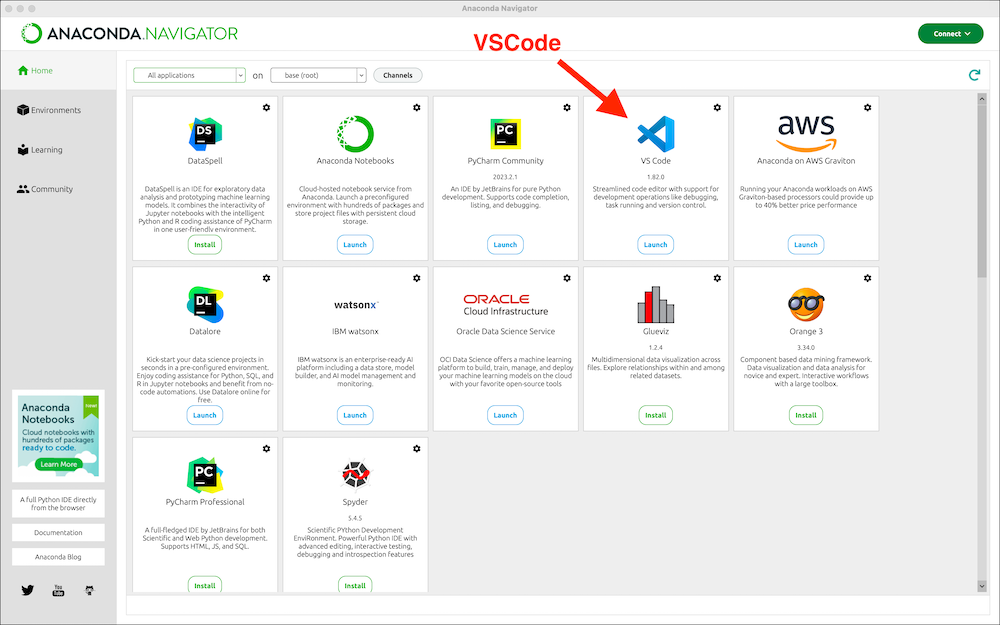
\includegraphics{basics/anaconda-navigator.png}

Sometimes you will need to manualy install the Jupyter extension on
VSCode. In this case follow
\href{https://code.visualstudio.com/docs/datascience/jupyter-notebooks}{this
tutorial}.

\hypertarget{folder-structure}{%
\section{folder structure}\label{folder-structure}}

You \textbf{NEED} to be confortable with you computer's folder (or
directory) structure. Where are files located? How to navigate through
different folders? How is my stuff organized? If you don't feel
\textbf{absolutely} comfortable with this, then read this,
\href{http://www2.westsussex.gov.uk/LearningandDevelopment/IT\%20Learning\%20Guides/Microsoft\%20Windows\%207/05\%20Working\%20with\%20folders.pdf}{Windows},
\href{https://recoverit.wondershare.com/mac-tips/mac-finder-tutorial-mac.html}{MacOS}.
If you use Linux then you surely know this stuff. \textbf{Make yourself
a ``time-series'' folder} wherever you want, and have it backed up
regularly (use Google Drive, Dropbox, do it manually, etc). ``My dog
deleted my files'' is not an excuse.

\hypertarget{numpy-pandas-matplotlib}{%
\chapter{numpy, pandas, matplotlib}\label{numpy-pandas-matplotlib}}

\begin{Shaded}
\begin{Highlighting}[]
\ImportTok{import}\NormalTok{ numpy }\ImportTok{as}\NormalTok{ np}
\ImportTok{import}\NormalTok{ pandas }\ImportTok{as}\NormalTok{ pd}
\ImportTok{import}\NormalTok{ matplotlib.pyplot }\ImportTok{as}\NormalTok{ plt}
\end{Highlighting}
\end{Shaded}

The three lines above are the most common way you will start every
project in this course.

\begin{itemize}
\tightlist
\item
  \textbf{numpy} = numerical python. This library has a ton useful
  mathematical functions, and most importantly, it has an object called
  \texttt{numpy\ array}, which is one of the most useful data structures
  we have for time series analysis.
\item
  \textbf{pandas} is built upon numpy, and allows us to easily
  manipulate data stored in \texttt{dataframes}, a fancy name for a
  table.
\item
  \textbf{pyplot} is a submodule of \texttt{matplotlib}, and allows us
  to beautifully plot data.
\end{itemize}

The best resource I know to get acquainted with all three packages is
\href{https://jakevdp.github.io/PythonDataScienceHandbook/index.html}{Python
Data Science Handbook, by Jake VanderPlas}. This is a free online book,
with excellent step by step examples.

\hypertarget{pandas}{%
\section{pandas}\label{pandas}}

We will primarily use the Pandas package to deal with data. Pandas has
become the standard Python tool to manipulate time series, and you
should get acquainted with its basic usage. This course will provide you
the opportunity to learn by example, but I'm sure we will only scratch
the surface, and you'll be left with lots of questions.

I provide below a (non-comprehensive) list of useful tutorials, they are
a good reference for the beginner and for the experienced user.

\begin{itemize}
\tightlist
\item
  \href{https://jakevdp.github.io/PythonDataScienceHandbook/index.html}{Python
  Data Science Handbook, by Jake VanderPlas}
\item
  \href{https://pandas.pydata.org/Pandas_Cheat_Sheet.pdf}{Data Wrangling
  with pandas Cheat Sheet}
\item
  \href{https://images.datacamp.com/image/upload/v1666944896/Marketing/Blog/Working_with_Dates_and_Times_Cheat_Sheet.pdf}{Working
  with Dates and Times in Python}
\item
  \href{https://www.webpages.uidaho.edu/~stevel/cheatsheets/Pandas\%20DataFrame\%20Notes_12pages.pdf}{Cheat
  Sheet: The pandas DataFrame Object}
\item
  \href{https://www.youtube.com/watch?v=ZyhVh-qRZPA\&list=PL-osiE80TeTsWmV9i9c58mdDCSskIFdDS\&pp=iAQB}{YouTube
  tutorials} by Corey Schafer
\end{itemize}

\hypertarget{pyplot}{%
\section{pyplot}\label{pyplot}}

Matplotlib, and its submodule pyplot, are probably the most common
Python plotting tool. Pyplot is both great and horrible:

\begin{itemize}
\tightlist
\item
  Great: you'll have absolutely full control of everything you want to
  plot. The sky is the limit.
\item
  Horrible: you'll cry as you do it, because there is so much to know,
  and it is not the most friendly plotting package.
\end{itemize}

Pyplot is \emph{object oriented}, so you will usually manipulate the
\textbf{axes} object like this.

\begin{Shaded}
\begin{Highlighting}[]
\ImportTok{import}\NormalTok{ matplotlib.pyplot }\ImportTok{as}\NormalTok{ plt}

\NormalTok{x }\OperatorTok{=}\NormalTok{ [}\DecValTok{1}\NormalTok{, }\DecValTok{2}\NormalTok{, }\DecValTok{3}\NormalTok{, }\DecValTok{4}\NormalTok{, }\DecValTok{5}\NormalTok{]}
\NormalTok{y }\OperatorTok{=}\NormalTok{ [}\DecValTok{1}\NormalTok{, }\DecValTok{4}\NormalTok{, }\DecValTok{2}\NormalTok{, }\DecValTok{0}\NormalTok{, }\DecValTok{3}\NormalTok{]}

\CommentTok{\# Figure with two plots}
\NormalTok{fig, (ax1, ax2) }\OperatorTok{=}\NormalTok{ plt.subplots(}\DecValTok{1}\NormalTok{, }\DecValTok{2}\NormalTok{, figsize }\OperatorTok{=}\NormalTok{ (}\DecValTok{8}\NormalTok{, }\DecValTok{6}\NormalTok{))}
\CommentTok{\# plot on the left}
\NormalTok{ax1.plot(x, y, color}\OperatorTok{=}\StringTok{"tab:blue"}\NormalTok{)}
\NormalTok{ax1.plot(x, y[::}\OperatorTok{{-}}\DecValTok{1}\NormalTok{], color}\OperatorTok{=}\StringTok{"tab:orange"}\NormalTok{)}
\NormalTok{ax1.}\BuiltInTok{set}\NormalTok{(xlabel}\OperatorTok{=}\StringTok{"date"}\NormalTok{,}
\NormalTok{        ylabel}\OperatorTok{=}\StringTok{"something"}\NormalTok{,}
\NormalTok{        title}\OperatorTok{=}\StringTok{"left panel"}\NormalTok{)}
\CommentTok{\# plot on the right}
\NormalTok{ax2.plot(x, y[::}\OperatorTok{{-}}\DecValTok{1}\NormalTok{])}
\NormalTok{ax2.}\BuiltInTok{set}\NormalTok{(xlabel}\OperatorTok{=}\StringTok{"date"}\NormalTok{,}
\NormalTok{        ylabel}\OperatorTok{=}\StringTok{"something else"}\NormalTok{,}
\NormalTok{        title}\OperatorTok{=}\StringTok{"right panel"}\NormalTok{)}
\end{Highlighting}
\end{Shaded}

\begin{verbatim}
[Text(0.5, 0, 'date'),
 Text(0, 0.5, 'something else'),
 Text(0.5, 1.0, 'right panel')]
\end{verbatim}

\begin{figure}[H]

{\centering 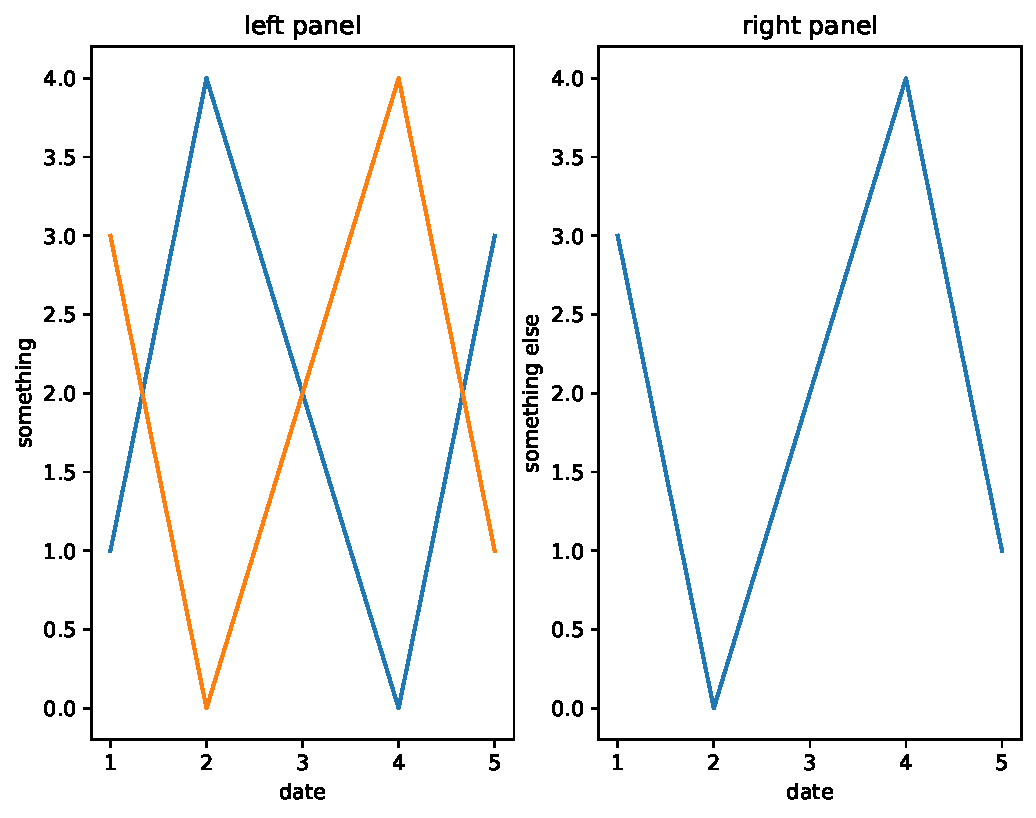
\includegraphics{basics/numpy-pandas-matplotlib_files/figure-pdf/cell-2-output-2.pdf}

}

\end{figure}

For the very beginners, you need to know that \texttt{figure} refers to
the whole white canvas, and \texttt{axes} means the rectangle inside
which something will be plotted:

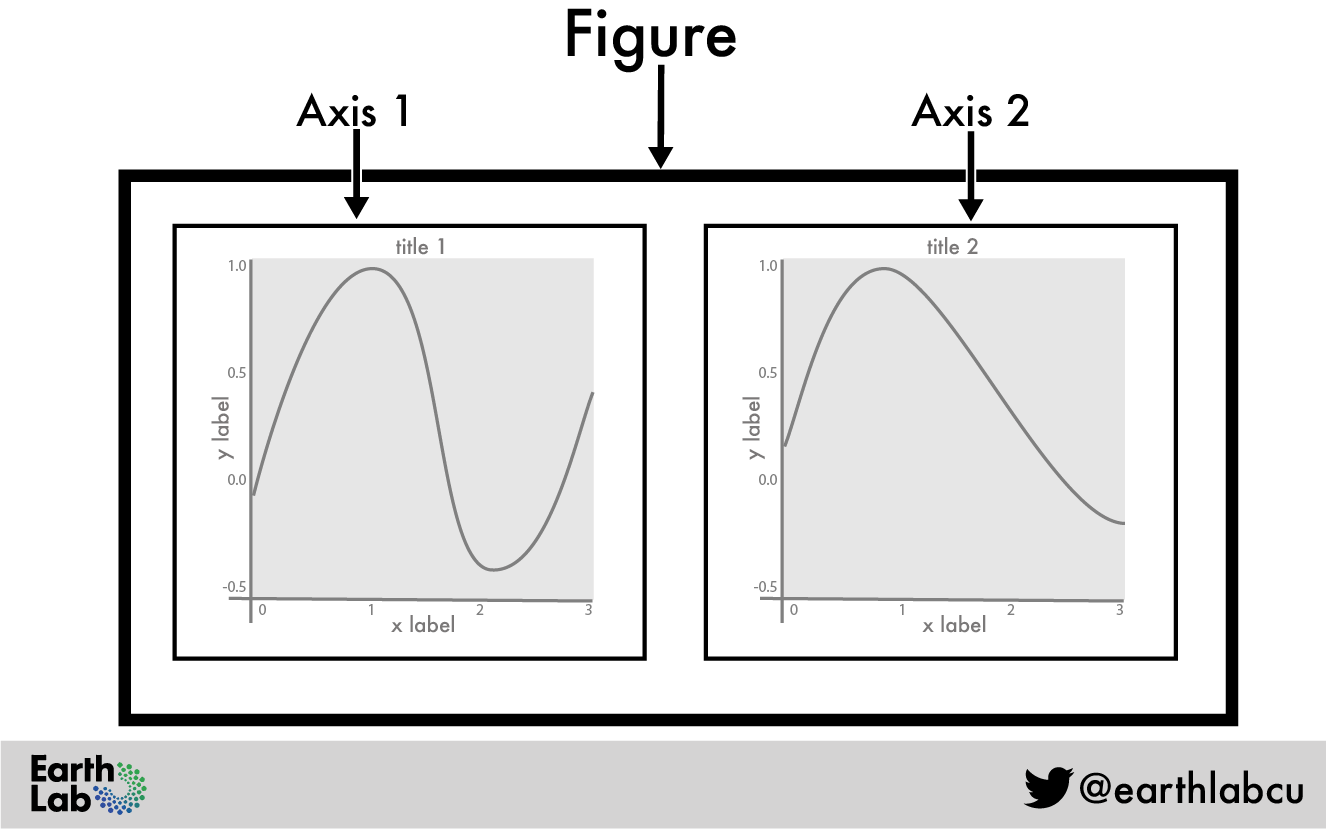
\includegraphics{basics/fig-2-plots.png}

The image above is good because it has 2 panels, and it's easy to
understand what going on. Sadly, they mixed the two terms, axis and
axes.

\begin{itemize}
\tightlist
\item
  \textbf{axes} is where the whole plot will be drawn. In the figure
  above it is the same as each panel.
\item
  \textbf{axis} is each of the vertical and horizontal lines, where you
  have ticks and numbers.
\end{itemize}

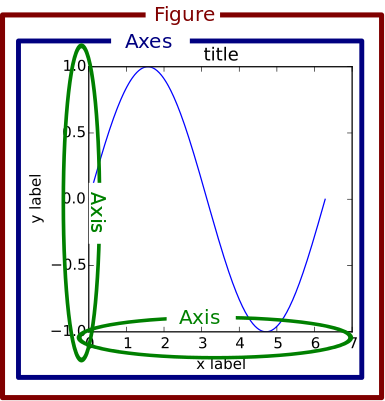
\includegraphics{basics/axis-vs-axes.png}

If you are new to all this, I recommend that you go to:

\begin{itemize}
\tightlist
\item
  \href{https://www.earthdatascience.org/courses/scientists-guide-to-plotting-data-in-python/plot-with-matplotlib/introduction-to-matplotlib-plots/}{Earth
  Lab's Introduction to Plotting in Python Using Matplotlib}
\item
  \href{https://jakevdp.github.io/PythonDataScienceHandbook/index.html}{Jake
  VanderPlas's Python Data Science Handbook}
\end{itemize}

\hypertarget{learn-by-example}{%
\chapter{learn by example}\label{learn-by-example}}

Now that everything is installed, try to run the code below
\emph{before} the first lecture. Don't worry if you don't understand
everything.

\begin{itemize}
\tightlist
\item
  If you manage to run everything without errors, this means that your
  computer is good to go!
\item
  You might encounter a few problems. That's ok. Make a note and we will
  solve everything in the first lecture.
\end{itemize}

Let's make a first plot of real data. We will use NOAA's Global
Monitoring Laboratory data on
\href{https://gml.noaa.gov/ccgg/trends/data.html}{Trends in Atmospheric
Carbon Dioxide}.

\hypertarget{open-a-new-jupyter-notebook}{%
\section{open a new Jupyter
Notebook}\label{open-a-new-jupyter-notebook}}

\begin{enumerate}
\def\labelenumi{\arabic{enumi}.}
\tightlist
\item
  On your computer, open the program \texttt{Anaconda\ Navigator} (it
  may take a while to load).
\item
  Find the white box called \texttt{VS\ Code} and click \texttt{Launch}.
\item
  Now go to \texttt{File} \textgreater{} \texttt{Open\ Folder}, and open
  the folder you created for this course. VS Code may ask you if you
  trust the authors, and the answer is ``yes'' (it's your computer).
\item
  \texttt{File} \textgreater{} \texttt{New\ File}, and call it
  \texttt{example.ipynb}
\item
  You can start copying and pasting code from this website to your
  Jupyter Notebook. To run a cell, press Shift+Enter.
\item
  You may be asked to choose to Select Kernel. This is VS Code wanting
  to know which python installation to use. Click on ``Python
  Environments'', and then choose the option with the word
  \texttt{anaconda} in it.
\item
  That's all! Congratulations!
\end{enumerate}

\hypertarget{import-packages}{%
\section{import packages}\label{import-packages}}

First, import packages to be used. They should all be already included
in the Anaconda distribution you installed.

\begin{Shaded}
\begin{Highlighting}[]
\ImportTok{import}\NormalTok{ numpy }\ImportTok{as}\NormalTok{ np}
\ImportTok{import}\NormalTok{ matplotlib.pyplot }\ImportTok{as}\NormalTok{ plt}
\ImportTok{import}\NormalTok{ pandas }\ImportTok{as}\NormalTok{ pd}
\ImportTok{import}\NormalTok{ seaborn }\ImportTok{as}\NormalTok{ sns}
\NormalTok{sns.}\BuiltInTok{set}\NormalTok{(style}\OperatorTok{=}\StringTok{"ticks"}\NormalTok{, font\_scale}\OperatorTok{=}\FloatTok{1.5}\NormalTok{)  }\CommentTok{\# white graphs, with large and legible letters}
\end{Highlighting}
\end{Shaded}

\hypertarget{load-data}{%
\section{load data}\label{load-data}}

Load CO2 data into a Pandas dataframe. You can load it directly from the
URL (option 1), or first download the CSV to your computer and then load
it (option 2). The link to download the data directly form NOAA is
\href{https://gml.noaa.gov/webdata/ccgg/trends/co2/co2_weekly_mlo.csv}{this}.
If for some reason this doesn't work, download here.

\begin{Shaded}
\begin{Highlighting}[]
\CommentTok{\# option 1: load data directly from URL}
\CommentTok{\# url = "https://gml.noaa.gov/webdata/ccgg/trends/co2/co2\_weekly\_mlo.csv"}
\CommentTok{\# df = pd.read\_csv(url,}
\CommentTok{\#                  header=34,}
\CommentTok{\#                  na\_values=[{-}999.99]}
\CommentTok{\#                  )}

\CommentTok{\# option 2: download first (use the URL above and save it to your computer), then load csv}
\NormalTok{filename }\OperatorTok{=} \StringTok{"co2\_weekly\_mlo.csv"}
\NormalTok{df }\OperatorTok{=}\NormalTok{ pd.read\_csv(filename,}
\NormalTok{                comment}\OperatorTok{=}\StringTok{\textquotesingle{}\#\textquotesingle{}}\NormalTok{,  }\CommentTok{\# will ignore rows starting with \#}
\NormalTok{                 na\_values}\OperatorTok{=}\NormalTok{[}\OperatorTok{{-}}\FloatTok{999.99}\NormalTok{]  }\CommentTok{\# substitute {-}999.99 for NaN (Not a Number), data not available}
\NormalTok{                 )}
\CommentTok{\# check how the dataframe (table) looks like}
\NormalTok{df}
\end{Highlighting}
\end{Shaded}

\begin{longtable}[]{@{}llllllllll@{}}
\toprule\noalign{}
& year & month & day & decimal & average & ndays & 1 year ago & 10 years
ago & increase since 1800 \\
\midrule\noalign{}
\endhead
\bottomrule\noalign{}
\endlastfoot
0 & 1974 & 5 & 19 & 1974.3795 & 333.37 & 5 & NaN & NaN & 50.39 \\
1 & 1974 & 5 & 26 & 1974.3986 & 332.95 & 6 & NaN & NaN & 50.05 \\
2 & 1974 & 6 & 2 & 1974.4178 & 332.35 & 5 & NaN & NaN & 49.59 \\
3 & 1974 & 6 & 9 & 1974.4370 & 332.20 & 7 & NaN & NaN & 49.64 \\
4 & 1974 & 6 & 16 & 1974.4562 & 332.37 & 7 & NaN & NaN & 50.06 \\
... & ... & ... & ... & ... & ... & ... & ... & ... & ... \\
2566 & 2023 & 7 & 23 & 2023.5575 & 421.28 & 4 & 418.03 & 397.30 &
141.60 \\
2567 & 2023 & 7 & 30 & 2023.5767 & 420.83 & 6 & 418.10 & 396.80 &
141.69 \\
2568 & 2023 & 8 & 6 & 2023.5959 & 420.02 & 6 & 417.36 & 395.65 &
141.41 \\
2569 & 2023 & 8 & 13 & 2023.6151 & 418.98 & 4 & 417.25 & 395.24 &
140.89 \\
2570 & 2023 & 8 & 20 & 2023.6342 & 419.31 & 2 & 416.64 & 395.22 &
141.71 \\
\end{longtable}

\hypertarget{dealing-with-dates}{%
\section{dealing with dates}\label{dealing-with-dates}}

Create a new column called \texttt{date}, that combines the information
from three separate columns: \texttt{year}, \texttt{month},
\texttt{day}.

\begin{Shaded}
\begin{Highlighting}[]
\CommentTok{\# function to\_datetime translates the full date into a pandas datetime object,}
\CommentTok{\# that is, pandas knows this is a date, it\textquotesingle{}s not just a string}
\NormalTok{df[}\StringTok{\textquotesingle{}date\textquotesingle{}}\NormalTok{] }\OperatorTok{=}\NormalTok{ pd.to\_datetime(df[[}\StringTok{\textquotesingle{}year\textquotesingle{}}\NormalTok{, }\StringTok{\textquotesingle{}month\textquotesingle{}}\NormalTok{, }\StringTok{\textquotesingle{}day\textquotesingle{}}\NormalTok{]])}
\CommentTok{\# make \textquotesingle{}date\textquotesingle{} column the dataframe index}
\NormalTok{df }\OperatorTok{=}\NormalTok{ df.set\_index(}\StringTok{\textquotesingle{}date\textquotesingle{}}\NormalTok{)}
\CommentTok{\# now see if everything is ok}
\NormalTok{df}
\end{Highlighting}
\end{Shaded}

\begin{longtable}[]{@{}llllllllll@{}}
\toprule\noalign{}
& year & month & day & decimal & average & ndays & 1 year ago & 10 years
ago & increase since 1800 \\
date & & & & & & & & & \\
\midrule\noalign{}
\endhead
\bottomrule\noalign{}
\endlastfoot
1974-05-19 & 1974 & 5 & 19 & 1974.3795 & 333.37 & 5 & NaN & NaN &
50.39 \\
1974-05-26 & 1974 & 5 & 26 & 1974.3986 & 332.95 & 6 & NaN & NaN &
50.05 \\
1974-06-02 & 1974 & 6 & 2 & 1974.4178 & 332.35 & 5 & NaN & NaN &
49.59 \\
1974-06-09 & 1974 & 6 & 9 & 1974.4370 & 332.20 & 7 & NaN & NaN &
49.64 \\
1974-06-16 & 1974 & 6 & 16 & 1974.4562 & 332.37 & 7 & NaN & NaN &
50.06 \\
... & ... & ... & ... & ... & ... & ... & ... & ... & ... \\
2023-07-23 & 2023 & 7 & 23 & 2023.5575 & 421.28 & 4 & 418.03 & 397.30 &
141.60 \\
2023-07-30 & 2023 & 7 & 30 & 2023.5767 & 420.83 & 6 & 418.10 & 396.80 &
141.69 \\
2023-08-06 & 2023 & 8 & 6 & 2023.5959 & 420.02 & 6 & 417.36 & 395.65 &
141.41 \\
2023-08-13 & 2023 & 8 & 13 & 2023.6151 & 418.98 & 4 & 417.25 & 395.24 &
140.89 \\
2023-08-20 & 2023 & 8 & 20 & 2023.6342 & 419.31 & 2 & 416.64 & 395.22 &
141.71 \\
\end{longtable}

\hypertarget{first-plot}{%
\section{first plot}\label{first-plot}}

We are now ready for our first plot! Let's see the weekly CO2 average.

\begin{Shaded}
\begin{Highlighting}[]
\CommentTok{\# \%matplotlib widget}
\CommentTok{\# uncomment the above line if you want dynamic control of the figure when using VSCode}
\NormalTok{fig, (ax1, ax2) }\OperatorTok{=}\NormalTok{ plt.subplots(}\DecValTok{1}\NormalTok{, }\DecValTok{2}\NormalTok{,  }\CommentTok{\# 1 row, 2 columns}
\NormalTok{                               figsize}\OperatorTok{=}\NormalTok{(}\DecValTok{8}\NormalTok{,}\DecValTok{5}\NormalTok{)  }\CommentTok{\# width, height, in inches}
\NormalTok{                               )}
\CommentTok{\# left panel}
\NormalTok{ax1.plot(df[}\StringTok{\textquotesingle{}average\textquotesingle{}}\NormalTok{], color}\OperatorTok{=}\StringTok{"black"}\NormalTok{)}
\NormalTok{ax1.plot(df.loc[}\StringTok{\textquotesingle{}2010{-}01{-}01\textquotesingle{}}\NormalTok{:}\StringTok{\textquotesingle{}2011{-}12{-}31\textquotesingle{}}\NormalTok{,}\StringTok{\textquotesingle{}average\textquotesingle{}}\NormalTok{], color}\OperatorTok{=}\StringTok{"magenta"}\NormalTok{)}
\NormalTok{ax1.}\BuiltInTok{set}\NormalTok{(xlabel}\OperatorTok{=}\StringTok{"date"}\NormalTok{,}
\NormalTok{       ylabel}\OperatorTok{=}\VerbatimStringTok{r"CO$\_2$ concentration (ppm)"}\NormalTok{,}
\NormalTok{       title}\OperatorTok{=}\StringTok{"long term"}\NormalTok{)}\OperatorTok{;}
\CommentTok{\# right panel}
\NormalTok{ax2.plot(df.loc[}\StringTok{\textquotesingle{}2010{-}01{-}01\textquotesingle{}}\NormalTok{:}\StringTok{\textquotesingle{}2011{-}12{-}31\textquotesingle{}}\NormalTok{,}\StringTok{\textquotesingle{}average\textquotesingle{}}\NormalTok{], color}\OperatorTok{=}\StringTok{"magenta"}\NormalTok{)}
\NormalTok{ax2.}\BuiltInTok{set}\NormalTok{(xlabel}\OperatorTok{=}\StringTok{"date"}\NormalTok{,}
\NormalTok{        ylabel}\OperatorTok{=}\VerbatimStringTok{r"CO$\_2$ concentration (ppm)"}\NormalTok{,}
\NormalTok{        ylim}\OperatorTok{=}\NormalTok{[}\DecValTok{385}\NormalTok{, }\DecValTok{400}\NormalTok{],  }\CommentTok{\# choose y limits}
\NormalTok{        yticks}\OperatorTok{=}\NormalTok{np.arange(}\DecValTok{385}\NormalTok{, }\DecValTok{401}\NormalTok{, }\DecValTok{5}\NormalTok{),  }\CommentTok{\# choose ticks}
\NormalTok{        title}\OperatorTok{=}\StringTok{"years 2010{-}{-}2011"}\NormalTok{)}\OperatorTok{;}
\CommentTok{\# put ticks and label on the right for ax2}
\NormalTok{ax2.yaxis.tick\_right()}
\NormalTok{ax2.yaxis.set\_label\_position(}\StringTok{"right"}\NormalTok{)}
\CommentTok{\# title above both panels}
\NormalTok{fig.suptitle(}\StringTok{"Mauna Loa Observatory"}\NormalTok{)}
\CommentTok{\# makes slanted dates}
\NormalTok{plt.gcf().autofmt\_xdate()}
\end{Highlighting}
\end{Shaded}

\begin{figure}[H]

{\centering \includegraphics{basics/example_files/figure-pdf/cell-5-output-1.png}

}

\end{figure}

\hypertarget{first-plot-v2.0}{%
\section{first plot, v2.0}\label{first-plot-v2.0}}

The dates in the x-label are not great. Let's try to make them prettier.

We need to import a few more packages first.

\begin{Shaded}
\begin{Highlighting}[]
\ImportTok{import}\NormalTok{ matplotlib.dates }\ImportTok{as}\NormalTok{ mdates}
\ImportTok{from}\NormalTok{ matplotlib.dates }\ImportTok{import}\NormalTok{ DateFormatter}
\ImportTok{from}\NormalTok{ pandas.plotting }\ImportTok{import}\NormalTok{ register\_matplotlib\_converters}
\NormalTok{register\_matplotlib\_converters()  }\CommentTok{\# datetime converter for a matplotlib}
\end{Highlighting}
\end{Shaded}

Now let's replot.

\begin{Shaded}
\begin{Highlighting}[]
\CommentTok{\# \%matplotlib widget}
\CommentTok{\# uncomment the above line if you want dynamic control of the figure when using VSCode}
\NormalTok{fig, (ax1, ax2) }\OperatorTok{=}\NormalTok{ plt.subplots(}\DecValTok{1}\NormalTok{, }\DecValTok{2}\NormalTok{,  }\CommentTok{\# 1 row, 2 columns}
\NormalTok{                               figsize}\OperatorTok{=}\NormalTok{(}\DecValTok{8}\NormalTok{,}\DecValTok{5}\NormalTok{)  }\CommentTok{\# width, height, in inches}
\NormalTok{                               )}
\CommentTok{\# left panel}
\NormalTok{ax1.plot(df[}\StringTok{\textquotesingle{}average\textquotesingle{}}\NormalTok{], color}\OperatorTok{=}\StringTok{"black"}\NormalTok{)}
\NormalTok{ax1.plot(df.loc[}\StringTok{\textquotesingle{}2010{-}01{-}01\textquotesingle{}}\NormalTok{:}\StringTok{\textquotesingle{}2011{-}12{-}31\textquotesingle{}}\NormalTok{,}\StringTok{\textquotesingle{}average\textquotesingle{}}\NormalTok{], color}\OperatorTok{=}\StringTok{"magenta"}\NormalTok{)}
\NormalTok{ax1.}\BuiltInTok{set}\NormalTok{(xlabel}\OperatorTok{=}\StringTok{"date"}\NormalTok{,}
\NormalTok{       ylabel}\OperatorTok{=}\VerbatimStringTok{r"CO$\_2$ concentration (ppm)"}\NormalTok{,}
\NormalTok{       title}\OperatorTok{=}\StringTok{"long term"}\NormalTok{)}\OperatorTok{;}
\CommentTok{\# right panel}
\NormalTok{ax2.plot(df.loc[}\StringTok{\textquotesingle{}2010{-}01{-}01\textquotesingle{}}\NormalTok{:}\StringTok{\textquotesingle{}2011{-}12{-}31\textquotesingle{}}\NormalTok{,}\StringTok{\textquotesingle{}average\textquotesingle{}}\NormalTok{], color}\OperatorTok{=}\StringTok{"magenta"}\NormalTok{)}
\NormalTok{ax2.}\BuiltInTok{set}\NormalTok{(xlabel}\OperatorTok{=}\StringTok{"date"}\NormalTok{,}
\NormalTok{        ylabel}\OperatorTok{=}\VerbatimStringTok{r"CO$\_2$ concentration (ppm)"}\NormalTok{,}
\NormalTok{        ylim}\OperatorTok{=}\NormalTok{[}\DecValTok{385}\NormalTok{, }\DecValTok{400}\NormalTok{],  }\CommentTok{\# choose y limits}
\NormalTok{        yticks}\OperatorTok{=}\NormalTok{np.arange(}\DecValTok{385}\NormalTok{, }\DecValTok{401}\NormalTok{, }\DecValTok{5}\NormalTok{),  }\CommentTok{\# choose ticks}
\NormalTok{        title}\OperatorTok{=}\StringTok{"years 2010{-}{-}2011"}\NormalTok{)}\OperatorTok{;}
\CommentTok{\# put ticks and label on the right for ax2}
\NormalTok{ax2.yaxis.tick\_right()}
\NormalTok{ax2.yaxis.set\_label\_position(}\StringTok{"right"}\NormalTok{)}
\CommentTok{\# title above both panels}
\NormalTok{fig.suptitle(}\StringTok{"Mauna Loa Observatory"}\NormalTok{, y}\OperatorTok{=}\FloatTok{1.00}\NormalTok{)}

\NormalTok{locator }\OperatorTok{=}\NormalTok{ mdates.AutoDateLocator(minticks}\OperatorTok{=}\DecValTok{3}\NormalTok{, maxticks}\OperatorTok{=}\DecValTok{5}\NormalTok{)}
\NormalTok{formatter }\OperatorTok{=}\NormalTok{ mdates.ConciseDateFormatter(locator)}
\NormalTok{ax1.xaxis.set\_major\_locator(locator)}
\NormalTok{ax1.xaxis.set\_major\_formatter(formatter)}

\NormalTok{locator }\OperatorTok{=}\NormalTok{ mdates.AutoDateLocator(minticks}\OperatorTok{=}\DecValTok{4}\NormalTok{, maxticks}\OperatorTok{=}\DecValTok{5}\NormalTok{)}
\NormalTok{formatter }\OperatorTok{=}\NormalTok{ mdates.ConciseDateFormatter(locator)}
\NormalTok{ax2.xaxis.set\_major\_locator(locator)}
\NormalTok{ax2.xaxis.set\_major\_formatter(formatter)}

\NormalTok{ax1.annotate(}
    \StringTok{"2010/11"}\NormalTok{,}
\NormalTok{    xy}\OperatorTok{=}\NormalTok{(}\StringTok{\textquotesingle{}2011{-}12{-}25\textquotesingle{}}\NormalTok{, }\DecValTok{389}\NormalTok{),  xycoords}\OperatorTok{=}\StringTok{\textquotesingle{}data\textquotesingle{}}\NormalTok{,}
\NormalTok{    xytext}\OperatorTok{=}\NormalTok{(}\OperatorTok{{-}}\DecValTok{10}\NormalTok{, }\OperatorTok{{-}}\DecValTok{80}\NormalTok{), textcoords}\OperatorTok{=}\StringTok{\textquotesingle{}offset points\textquotesingle{}}\NormalTok{,}
\NormalTok{    arrowprops}\OperatorTok{=}\BuiltInTok{dict}\NormalTok{(arrowstyle}\OperatorTok{=}\StringTok{"{-}\textgreater{}"}\NormalTok{,}
\NormalTok{                    color}\OperatorTok{=}\StringTok{"black"}\NormalTok{,}
\NormalTok{                    connectionstyle}\OperatorTok{=}\StringTok{"arc3,rad=0.2"}\NormalTok{))}
\NormalTok{fig.savefig(}\StringTok{"CO2{-}graph.png"}\NormalTok{, dpi}\OperatorTok{=}\DecValTok{300}\NormalTok{)}
\end{Highlighting}
\end{Shaded}

\begin{verbatim}
/var/folders/hc/jhnmlst937d27zzq9fhfks780000gn/T/ipykernel_10652/850389963.py:42: UserWarning: AutoDateLocator was unable to pick an appropriate interval for this date range. It may be necessary to add an interval value to the AutoDateLocator's intervald dictionary. Defaulting to 6.
  fig.savefig("CO2-graph.png", dpi=300)
/opt/anaconda3/lib/python3.9/site-packages/IPython/core/pylabtools.py:151: UserWarning: AutoDateLocator was unable to pick an appropriate interval for this date range. It may be necessary to add an interval value to the AutoDateLocator's intervald dictionary. Defaulting to 6.
  fig.canvas.print_figure(bytes_io, **kw)
\end{verbatim}

\begin{figure}[H]

{\centering 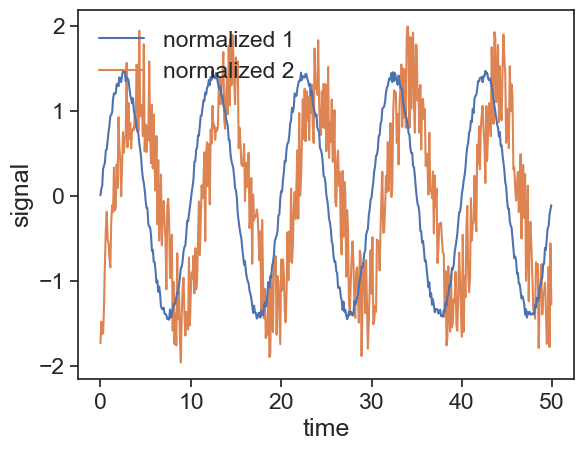
\includegraphics{basics/example_files/figure-pdf/cell-7-output-2.png}

}

\end{figure}

The dates on the horizontal axis are determined thus:

\begin{enumerate}
\def\labelenumi{\arabic{enumi}.}
\tightlist
\item
  \texttt{locator\ =\ mdates.AutoDateLocator(minticks=3,\ maxticks=5)}\strut \\
  This deremines the location of the ticks (between 3 and 5 ticks,
  whatever ``works best'')
\item
  \texttt{ax1.xaxis.set\_major\_locator(locator)}\strut \\
  This actually puts the ticks in the positions determined above
\item
  \texttt{formatter\ =\ mdates.ConciseDateFormatter(locator)}\strut \\
  This says that the labels will be placed at the locations determined
  in 1.
\item
  \texttt{ax1.xaxis.set\_major\_formatter(formatter)}\strut \\
  Finally, labels are written down
\end{enumerate}

The arrow is placed in the graph using \texttt{annotate}. It has a
tricky syntax and a million options. Read
\href{https://jakevdp.github.io/PythonDataScienceHandbook/04.09-text-and-annotation.html\#Arrows-and-Annotation}{Jake
VanderPlas's} excellent examples to learn more.

\hypertarget{modifications}{%
\section{modifications}\label{modifications}}

Let's change a lot of plotting options to see how things could be
different.

\begin{Shaded}
\begin{Highlighting}[]
\NormalTok{sns.}\BuiltInTok{set}\NormalTok{(style}\OperatorTok{=}\StringTok{"darkgrid"}\NormalTok{)}
\NormalTok{sns.set\_context(}\StringTok{"notebook"}\NormalTok{)}

\CommentTok{\# \%matplotlib widget}
\CommentTok{\# uncomment the above line if you want dynamic control of the figure when using VSCode}
\NormalTok{fig, (ax1, ax2) }\OperatorTok{=}\NormalTok{ plt.subplots(}\DecValTok{1}\NormalTok{, }\DecValTok{2}\NormalTok{,  }\CommentTok{\# 1 row, 2 columns}
\NormalTok{                               figsize}\OperatorTok{=}\NormalTok{(}\DecValTok{8}\NormalTok{,}\DecValTok{4}\NormalTok{)  }\CommentTok{\# width, height, in inches}
\NormalTok{                               )}
\CommentTok{\# left panel}
\NormalTok{ax1.plot(df[}\StringTok{\textquotesingle{}average\textquotesingle{}}\NormalTok{], color}\OperatorTok{=}\StringTok{"tab:blue"}\NormalTok{)}
\NormalTok{ax1.plot(df.loc[}\StringTok{\textquotesingle{}2010{-}01{-}01\textquotesingle{}}\NormalTok{:}\StringTok{\textquotesingle{}2011{-}12{-}31\textquotesingle{}}\NormalTok{,}\StringTok{\textquotesingle{}average\textquotesingle{}}\NormalTok{], color}\OperatorTok{=}\StringTok{"tab:orange"}\NormalTok{)}
\NormalTok{ax1.}\BuiltInTok{set}\NormalTok{(xlabel}\OperatorTok{=}\StringTok{"date"}\NormalTok{,}
\NormalTok{       ylabel}\OperatorTok{=}\VerbatimStringTok{r"CO$\_2$ concentration (ppm)"}\NormalTok{,}
\NormalTok{       title}\OperatorTok{=}\StringTok{"long term"}\NormalTok{)}\OperatorTok{;}
\CommentTok{\# right panel}
\NormalTok{ax2.plot(df.loc[}\StringTok{\textquotesingle{}2010{-}01{-}01\textquotesingle{}}\NormalTok{:}\StringTok{\textquotesingle{}2011{-}12{-}31\textquotesingle{}}\NormalTok{,}\StringTok{\textquotesingle{}average\textquotesingle{}}\NormalTok{], color}\OperatorTok{=}\StringTok{"tab:orange"}\NormalTok{)}
\NormalTok{ax2.}\BuiltInTok{set}\NormalTok{(xlabel}\OperatorTok{=}\StringTok{"date"}\NormalTok{,}
\NormalTok{        ylim}\OperatorTok{=}\NormalTok{[}\DecValTok{385}\NormalTok{, }\DecValTok{400}\NormalTok{],  }\CommentTok{\# choose y limits}
\NormalTok{        yticks}\OperatorTok{=}\NormalTok{np.arange(}\DecValTok{385}\NormalTok{, }\DecValTok{401}\NormalTok{, }\DecValTok{5}\NormalTok{),  }\CommentTok{\# choose ticks}
\NormalTok{        title}\OperatorTok{=}\StringTok{"years 2010{-}{-}2011"}\NormalTok{)}\OperatorTok{;}
\CommentTok{\# title above both panels}
\NormalTok{fig.suptitle(}\StringTok{"Mauna Loa Observatory"}\NormalTok{, y}\OperatorTok{=}\FloatTok{1.00}\NormalTok{)}

\NormalTok{locator }\OperatorTok{=}\NormalTok{ mdates.AutoDateLocator(minticks}\OperatorTok{=}\DecValTok{3}\NormalTok{, maxticks}\OperatorTok{=}\DecValTok{5}\NormalTok{)}
\NormalTok{formatter }\OperatorTok{=}\NormalTok{ mdates.ConciseDateFormatter(locator)}
\NormalTok{ax1.xaxis.set\_major\_locator(locator)}
\NormalTok{ax1.xaxis.set\_major\_formatter(formatter)}

\NormalTok{locator }\OperatorTok{=}\NormalTok{ mdates.AutoDateLocator(minticks}\OperatorTok{=}\DecValTok{5}\NormalTok{, maxticks}\OperatorTok{=}\DecValTok{8}\NormalTok{)}
\NormalTok{formatter }\OperatorTok{=}\NormalTok{ mdates.ConciseDateFormatter(locator)}
\NormalTok{ax2.xaxis.set\_major\_locator(locator)}
\NormalTok{ax2.xaxis.set\_major\_formatter(formatter)}

\NormalTok{ax1.annotate(}
    \StringTok{"2010/11"}\NormalTok{,}
\NormalTok{    xy}\OperatorTok{=}\NormalTok{(}\StringTok{\textquotesingle{}2010{-}12{-}25\textquotesingle{}}\NormalTok{, }\DecValTok{395}\NormalTok{),  xycoords}\OperatorTok{=}\StringTok{\textquotesingle{}data\textquotesingle{}}\NormalTok{,}
\NormalTok{    xytext}\OperatorTok{=}\NormalTok{(}\OperatorTok{{-}}\DecValTok{100}\NormalTok{, }\DecValTok{40}\NormalTok{), textcoords}\OperatorTok{=}\StringTok{\textquotesingle{}offset points\textquotesingle{}}\NormalTok{,}
\NormalTok{    bbox}\OperatorTok{=}\BuiltInTok{dict}\NormalTok{(boxstyle}\OperatorTok{=}\StringTok{"round4,pad=.5"}\NormalTok{, fc}\OperatorTok{=}\StringTok{"white"}\NormalTok{),}
\NormalTok{    arrowprops}\OperatorTok{=}\BuiltInTok{dict}\NormalTok{(arrowstyle}\OperatorTok{=}\StringTok{"{-}\textgreater{}"}\NormalTok{,}
\NormalTok{                    color}\OperatorTok{=}\StringTok{"black"}\NormalTok{,}
\NormalTok{                    connectionstyle}\OperatorTok{=}\StringTok{"angle,angleA=0,angleB={-}90,rad=40"}\NormalTok{))}
\end{Highlighting}
\end{Shaded}

\begin{verbatim}
Text(-100, 40, '2010/11')
\end{verbatim}

\begin{figure}[H]

{\centering 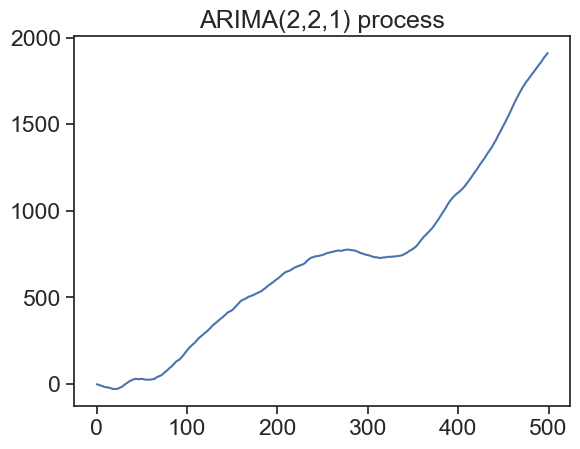
\includegraphics{basics/example_files/figure-pdf/cell-8-output-2.png}

}

\end{figure}

The main changes were:

\begin{enumerate}
\def\labelenumi{\arabic{enumi}.}
\tightlist
\item
  Using the Seaborn package, we changed the fontsize and the overall
  plot style.
  \href{https://seaborn.pydata.org/tutorial/aesthetics.html}{Read
  more}.\\
  \texttt{sns.set(style="darkgrid")}\strut \\
  \texttt{sns.set\_context("notebook")}
\item
  We changed the colors of the lineplots. To know what colors exist,
  \href{https://matplotlib.org/stable/gallery/color/named_colors.html}{click
  here}.
\item
  The arrow annotation has a different style.
  \href{https://jakevdp.github.io/PythonDataScienceHandbook/04.09-text-and-annotation.html\#Arrows-and-Annotation}{Read
  more}.
\end{enumerate}

\hypertarget{playing-with-the-code}{%
\section{playing with the code}\label{playing-with-the-code}}

I encourage you to play with the code you just ran. An easy way of
learning what each line does is to comment something out and see what
changes in the output you see. If you feel brave, try to modify the code
a little bit.

\hypertarget{ai-policy}{%
\chapter{AI policy}\label{ai-policy}}

\begin{figure}

{\centering 
\includegraphics[width=1.04167in,height=\textheight]{basics/robot-scratching_transparent3.png}

}

\end{figure}

The guidelines below are an adaptation of
\href{https://oneusefulthing.substack.com/p/all-my-classes-suddenly-became-ai}{Ethan
Mollick's extremely useful ideas on AI} as an assistant tool for
teaching.

\textbf{I EXPECT YOU} to use LLMs (large language models) such as
ChatGPT, Bing AI, Google Bard, or whatever else springs up since the
time of this writing. You should familiarize yourself with the AI's
capabilities and limitations.

\textbf{Use LLMs to help you learn}, chat with them about what you want
to accomplish and learn from them how to do it. \textbf{Ask} your LLM
what each part of the code means, copy and pasting blindly is
unacceptable. You are here to learn.

Consider the following important points:

\begin{itemize}
\tightlist
\item
  Ultimately, you, the student, are responsible for the assignment.
\item
  Acknowledge the use of AI in your assignment. Be transparent about
  your use of the tool and the extent of assistance it provided.
\end{itemize}

\begin{figure}

{\centering 
\includegraphics{basics/ai-meme1.png}

}

\end{figure}

\part{resampling}

\hypertarget{motivation}{%
\chapter{motivation}\label{motivation}}

\hypertarget{jerusalem-2019}{%
\section{Jerusalem, 2019}\label{jerusalem-2019}}

Data from the \href{https://ims.gov.il/en/data_gov}{Israel
Meteorological Service}, IMS.

See the temperature at a weather station in Jerusalem, for the whole
2019 year. This is an interactive graph: to zoom in, play with the
bottom panel.

\begin{verbatim}
alt.VConcatChart(...)
\end{verbatim}

\hypertarget{iconify-cil-chat-bubble-discussion}{%
\paragraph*{\texorpdfstring{
discussion}{ discussion}}\label{iconify-cil-chat-bubble-discussion}}
\addcontentsline{toc}{paragraph}{ discussion}

The temperature fluctuates on various time scales, from daily to yearly.
Let's think together a few questions we'd like to ask about the data
above.

Now let's see precipitation data:

\begin{verbatim}
alt.VConcatChart(...)
\end{verbatim}

\hypertarget{iconify-cil-chat-bubble-discussion-1}{%
\paragraph*{\texorpdfstring{
discussion}{ discussion}}\label{iconify-cil-chat-bubble-discussion-1}}
\addcontentsline{toc}{paragraph}{ discussion}

What would be interesting to know about precipitation?

We have not talked about what kind of data we have in our hands here.
The csv file provided by the IMS looks like this:

\begin{longtable}[]{@{}lllllllllllllllllll@{}}
\toprule\noalign{}
& Station & Date \& Time (Winter) & Diffused radiation (W/m\^{}2) &
Global radiation (W/m\^{}2) & Direct radiation (W/m\^{}2) & Relative
humidity (\%) & Temperature (°C) & Maximum temperature (°C) & Minimum
temperature (°C) & Wind direction (°) & Gust wind direction (°) & Wind
speed (m/s) & Maximum 1 minute wind speed (m/s) & Maximum 10 minutes
wind speed (m/s) & Time ending maximum 10 minutes wind speed (hhmm) &
Gust wind speed (m/s) & Standard deviation wind direction (°) & Rainfall
(mm) \\
\midrule\noalign{}
\endhead
\bottomrule\noalign{}
\endlastfoot
0 & Jerusalem Givat Ram & 01/01/2019 00:00 & 0.0 & 0.0 & 0.0 & 80.0 &
8.7 & 8.8 & 8.6 & 75.0 & 84.0 & 3.3 & 4.3 & 3.5 & 23:58 & 6.0 & 15.6 &
0.0 \\
1 & Jerusalem Givat Ram & 01/01/2019 00:10 & 0.0 & 0.0 & 0.0 & 79.0 &
8.7 & 8.8 & 8.7 & 74.0 & 82.0 & 3.3 & 4.1 & 3.3 & 00:01 & 4.9 & 14.3 &
0.0 \\
2 & Jerusalem Givat Ram & 01/01/2019 00:20 & 0.0 & 0.0 & 0.0 & 79.0 &
8.7 & 8.8 & 8.7 & 76.0 & 82.0 & 3.2 & 4.1 & 3.3 & 00:19 & 4.9 & 9.9 &
0.0 \\
3 & Jerusalem Givat Ram & 01/01/2019 00:30 & 0.0 & 0.0 & 0.0 & 79.0 &
8.7 & 8.7 & 8.6 & 78.0 & 73.0 & 3.6 & 4.2 & 3.6 & 00:30 & 5.2 & 11.7 &
0.0 \\
4 & Jerusalem Givat Ram & 01/01/2019 00:40 & 0.0 & 0.0 & 0.0 & 79.0 &
8.6 & 8.7 & 8.5 & 80.0 & 74.0 & 3.6 & 4.4 & 3.8 & 00:35 & 5.4 & 10.5 &
0.0 \\
... & ... & ... & ... & ... & ... & ... & ... & ... & ... & ... & ... &
... & ... & ... & ... & ... & ... & ... \\
52549 & Jerusalem Givat Ram & 31/12/2019 22:20 & 0.0 & 0.0 & 1.0 & 81.0
& 7.4 & 7.6 & 7.3 & 222.0 & 255.0 & 0.5 & 0.9 & 1.0 & 22:11 & 1.0 & 47.9
& 0.0 \\
52550 & Jerusalem Givat Ram & 31/12/2019 22:30 & 0.0 & 0.0 & 1.0 & 83.0
& 7.3 & 7.4 & 7.3 & 266.0 & 259.0 & 0.6 & 0.8 & 0.6 & 22:28 & 1.1 & 22.8
& 0.0 \\
52551 & Jerusalem Givat Ram & 31/12/2019 22:40 & 0.0 & 0.0 & 1.0 & 83.0
& 7.5 & 7.6 & 7.3 & 331.0 & 317.0 & 0.5 & 0.8 & 0.6 & 22:35 & 1.0 & 31.6
& 0.0 \\
52552 & Jerusalem Givat Ram & 31/12/2019 22:50 & 0.0 & 0.0 & 1.0 & 83.0
& 7.5 & 7.6 & 7.4 & 312.0 & 285.0 & 0.6 & 1.0 & 0.6 & 22:50 & 1.4 & 31.3
& 0.0 \\
52553 & Jerusalem Givat Ram & 31/12/2019 23:00 & 0.0 & 0.0 & 1.0 & 83.0
& 7.6 & 7.7 & 7.4 & 315.0 & 321.0 & 0.7 & 1.0 & 0.8 & 22:54 & 1.3 & 23.5
& 0.0 \\
\end{longtable}

We see that we have data points spaced out evenly every 10 minutes.

\hypertarget{challenges}{%
\section{Challenges}\label{challenges}}

Let's try to answer the following questions:

\begin{tcolorbox}[enhanced jigsaw, coltitle=black, colbacktitle=quarto-callout-note-color!10!white, arc=.35mm, colframe=quarto-callout-note-color-frame, leftrule=.75mm, opacitybacktitle=0.6, breakable, colback=white, left=2mm, title={What is the mean temperature for each month?}, opacityback=0, toprule=.15mm, titlerule=0mm, bottomtitle=1mm, rightrule=.15mm, bottomrule=.15mm, toptitle=1mm]

First we have to divide temperature data by month, and then take the
average for each month.

a possible solution

\begin{Shaded}
\begin{Highlighting}[]
\NormalTok{df\_month }\OperatorTok{=}\NormalTok{ df[}\StringTok{\textquotesingle{}temperature\textquotesingle{}}\NormalTok{].resample(}\StringTok{\textquotesingle{}M\textquotesingle{}}\NormalTok{).mean()}
\end{Highlighting}
\end{Shaded}

\end{tcolorbox}

\begin{tcolorbox}[enhanced jigsaw, coltitle=black, colbacktitle=quarto-callout-note-color!10!white, arc=.35mm, colframe=quarto-callout-note-color-frame, leftrule=.75mm, opacitybacktitle=0.6, breakable, colback=white, left=2mm, title={For each month, what is the mean of the daily maximum temperature? What
about the minimun?}, opacityback=0, toprule=.15mm, titlerule=0mm, bottomtitle=1mm, rightrule=.15mm, bottomrule=.15mm, toptitle=1mm]

This is a bit trickier.

\begin{enumerate}
\def\labelenumi{\arabic{enumi}.}
\tightlist
\item
  We need to find the maximum/minimum temperature for each day.
\item
  Only then we split the daily data by month and take the average.
\end{enumerate}

a possible solution

\begin{Shaded}
\begin{Highlighting}[]
\NormalTok{df\_day[}\StringTok{\textquotesingle{}max temp\textquotesingle{}}\NormalTok{] }\OperatorTok{=}\NormalTok{ df[}\StringTok{\textquotesingle{}temperature\textquotesingle{}}\NormalTok{].resample(}\StringTok{\textquotesingle{}D\textquotesingle{}}\NormalTok{).}\BuiltInTok{max}\NormalTok{()}
\NormalTok{df\_month[}\StringTok{\textquotesingle{}max temp\textquotesingle{}}\NormalTok{] }\OperatorTok{=}\NormalTok{ df\_day[}\StringTok{\textquotesingle{}max temp\textquotesingle{}}\NormalTok{].resample(}\StringTok{\textquotesingle{}MS\textquotesingle{}}\NormalTok{).mean()}
\end{Highlighting}
\end{Shaded}

\end{tcolorbox}

\begin{tcolorbox}[enhanced jigsaw, coltitle=black, colbacktitle=quarto-callout-note-color!10!white, arc=.35mm, colframe=quarto-callout-note-color-frame, leftrule=.75mm, opacitybacktitle=0.6, breakable, colback=white, left=2mm, title={What is the average night temperature for every season? What about the
day temperature?}, opacityback=0, toprule=.15mm, titlerule=0mm, bottomtitle=1mm, rightrule=.15mm, bottomrule=.15mm, toptitle=1mm]

\begin{enumerate}
\def\labelenumi{\arabic{enumi}.}
\tightlist
\item
  We need to filter our data to contain only night times.
\item
  We need to divide rain data by seasons (3 months), and then take the
  mean for each season.
\end{enumerate}

a possible solution

\begin{Shaded}
\begin{Highlighting}[]
\CommentTok{\# filter only night data}
\NormalTok{df\_night }\OperatorTok{=}\NormalTok{ df.loc[((df.index.hour }\OperatorTok{\textless{}} \DecValTok{6}\NormalTok{) }\OperatorTok{|}\NormalTok{ (df.index.hour }\OperatorTok{\textgreater{}=} \DecValTok{18}\NormalTok{))]}
\NormalTok{season\_average\_night\_temp }\OperatorTok{=}\NormalTok{ df\_night[}\StringTok{\textquotesingle{}temperature\textquotesingle{}}\NormalTok{].resample(}\StringTok{\textquotesingle{}Q\textquotesingle{}}\NormalTok{).mean()}
\end{Highlighting}
\end{Shaded}

another possible solution

\begin{Shaded}
\begin{Highlighting}[]
\CommentTok{\# filter using between\_time}
\NormalTok{df\_night }\OperatorTok{=}\NormalTok{ df.between\_time(}\StringTok{\textquotesingle{}18:00\textquotesingle{}}\NormalTok{, }\StringTok{\textquotesingle{}06:00\textquotesingle{}}\NormalTok{, inclusive}\OperatorTok{=}\StringTok{\textquotesingle{}left\textquotesingle{}}\NormalTok{)}
\NormalTok{season\_average\_night\_temp }\OperatorTok{=}\NormalTok{ df\_night[}\StringTok{\textquotesingle{}temperature\textquotesingle{}}\NormalTok{].resample(}\StringTok{\textquotesingle{}Q\textquotesingle{}}\NormalTok{).mean()}
\end{Highlighting}
\end{Shaded}

\end{tcolorbox}

\begin{tcolorbox}[enhanced jigsaw, coltitle=black, colbacktitle=quarto-callout-note-color!10!white, arc=.35mm, colframe=quarto-callout-note-color-frame, leftrule=.75mm, opacitybacktitle=0.6, breakable, colback=white, left=2mm, title={What is the daily precipitation?}, opacityback=0, toprule=.15mm, titlerule=0mm, bottomtitle=1mm, rightrule=.15mm, bottomrule=.15mm, toptitle=1mm]

First we have to divide rain data by day, and then take the sum for each
day.

a possible solution

\begin{Shaded}
\begin{Highlighting}[]
\NormalTok{daily\_precipitation }\OperatorTok{=}\NormalTok{ df[}\StringTok{\textquotesingle{}rain\textquotesingle{}}\NormalTok{].resample(}\StringTok{\textquotesingle{}D\textquotesingle{}}\NormalTok{).}\BuiltInTok{sum}\NormalTok{()}
\end{Highlighting}
\end{Shaded}

\end{tcolorbox}

\begin{tcolorbox}[enhanced jigsaw, coltitle=black, colbacktitle=quarto-callout-note-color!10!white, arc=.35mm, colframe=quarto-callout-note-color-frame, leftrule=.75mm, opacitybacktitle=0.6, breakable, colback=white, left=2mm, title={How much rain was there every month?}, opacityback=0, toprule=.15mm, titlerule=0mm, bottomtitle=1mm, rightrule=.15mm, bottomrule=.15mm, toptitle=1mm]

We have to divide rain data by month, and then sum the totals of each
month.

a possible solution

\begin{Shaded}
\begin{Highlighting}[]
\NormalTok{monthly\_precipitation }\OperatorTok{=}\NormalTok{ df[}\StringTok{\textquotesingle{}rain\textquotesingle{}}\NormalTok{].resample(}\StringTok{\textquotesingle{}M\textquotesingle{}}\NormalTok{).}\BuiltInTok{sum}\NormalTok{()}
\end{Highlighting}
\end{Shaded}

\end{tcolorbox}

\begin{tcolorbox}[enhanced jigsaw, coltitle=black, colbacktitle=quarto-callout-note-color!10!white, arc=.35mm, colframe=quarto-callout-note-color-frame, leftrule=.75mm, opacitybacktitle=0.6, breakable, colback=white, left=2mm, title={How many rainy days were there each month?}, opacityback=0, toprule=.15mm, titlerule=0mm, bottomtitle=1mm, rightrule=.15mm, bottomrule=.15mm, toptitle=1mm]

\begin{enumerate}
\def\labelenumi{\arabic{enumi}.}
\tightlist
\item
  We need to sum rain by day.
\item
  We need to count how many days are there each month where
  \texttt{rain\ \textgreater{}\ 0}.
\end{enumerate}

a possible solution

\begin{Shaded}
\begin{Highlighting}[]
\NormalTok{daily\_precipitation }\OperatorTok{=}\NormalTok{ df[}\StringTok{\textquotesingle{}rain\textquotesingle{}}\NormalTok{].resample(}\StringTok{\textquotesingle{}D\textquotesingle{}}\NormalTok{).}\BuiltInTok{sum}\NormalTok{()}
\NormalTok{only\_rainy\_days }\OperatorTok{=}\NormalTok{ daily\_precipitation.loc[daily\_precipitation }\OperatorTok{\textgreater{}} \DecValTok{0}\NormalTok{]}
\NormalTok{rain\_days\_per\_month }\OperatorTok{=}\NormalTok{ only\_rainy\_days.resample(}\StringTok{\textquotesingle{}M\textquotesingle{}}\NormalTok{).count()}
\end{Highlighting}
\end{Shaded}

\end{tcolorbox}

\begin{tcolorbox}[enhanced jigsaw, coltitle=black, colbacktitle=quarto-callout-note-color!10!white, arc=.35mm, colframe=quarto-callout-note-color-frame, leftrule=.75mm, opacitybacktitle=0.6, breakable, colback=white, left=2mm, title={How many days, hours, and minutes were between the last rain of the
season (Malkosh) to the first (Yoreh)?}, opacityback=0, toprule=.15mm, titlerule=0mm, bottomtitle=1mm, rightrule=.15mm, bottomrule=.15mm, toptitle=1mm]

\begin{enumerate}
\def\labelenumi{\arabic{enumi}.}
\tightlist
\item
  We need to divide our data into two: \texttt{rainy\_season\_1} and
  \texttt{rainy\_season\_2}.
\item
  We need to find the time of the last rain in
  \texttt{rainy\_season\_1}.
\item
  We need to find the time of the first rain in
  \texttt{rainy\_season\_2}.
\item
  We need to compute the time difference between the two dates.
\end{enumerate}

a possible solution

\begin{Shaded}
\begin{Highlighting}[]
\NormalTok{split\_date }\OperatorTok{=} \StringTok{\textquotesingle{}2019{-}08{-}01\textquotesingle{}}
\NormalTok{rainy\_season\_1 }\OperatorTok{=}\NormalTok{ df[:split\_date]  }\CommentTok{\# everything before split date}
\NormalTok{rainy\_season\_2 }\OperatorTok{=}\NormalTok{ df[split\_date:]  }\CommentTok{\# everything after split date}
\NormalTok{malkosh }\OperatorTok{=}\NormalTok{ rainy\_season\_1[}\StringTok{\textquotesingle{}rain\textquotesingle{}}\NormalTok{].loc[rainy\_season\_1[}\StringTok{\textquotesingle{}rain\textquotesingle{}}\NormalTok{] }\OperatorTok{\textgreater{}} \DecValTok{0}\NormalTok{].last\_valid\_index()}
\NormalTok{yoreh }\OperatorTok{=}\NormalTok{ rainy\_season\_2[}\StringTok{\textquotesingle{}rain\textquotesingle{}}\NormalTok{].loc[rainy\_season\_2[}\StringTok{\textquotesingle{}rain\textquotesingle{}}\NormalTok{] }\OperatorTok{\textgreater{}} \DecValTok{0}\NormalTok{].first\_valid\_index()}
\NormalTok{dry\_period }\OperatorTok{=}\NormalTok{ yoreh }\OperatorTok{{-}}\NormalTok{ malkosh}
\CommentTok{\# extracting days, hours, and minutes}
\NormalTok{days }\OperatorTok{=}\NormalTok{ dry\_period.days}
\NormalTok{hours }\OperatorTok{=}\NormalTok{ dry\_period.components.hours}
\NormalTok{minutes }\OperatorTok{=}\NormalTok{ dry\_period.components.minutes}
\BuiltInTok{print}\NormalTok{(}\SpecialStringTok{f\textquotesingle{}The dry period of 2019 was }\SpecialCharTok{\{}\NormalTok{days}\SpecialCharTok{\}}\SpecialStringTok{ days, }\SpecialCharTok{\{}\NormalTok{hours}\SpecialCharTok{\}}\SpecialStringTok{ hours and }\SpecialCharTok{\{}\NormalTok{minutes}\SpecialCharTok{\}}\SpecialStringTok{ minutes.\textquotesingle{}}\NormalTok{)}
\end{Highlighting}
\end{Shaded}

\end{tcolorbox}

\begin{tcolorbox}[enhanced jigsaw, coltitle=black, colbacktitle=quarto-callout-note-color!10!white, arc=.35mm, colframe=quarto-callout-note-color-frame, leftrule=.75mm, opacitybacktitle=0.6, breakable, colback=white, left=2mm, title=\textcolor{quarto-callout-note-color}{\faInfo}\hspace{0.5em}{What was the rainiest morning (6am-12pm) of the year? Bonus, what about
the rainiest night (6pm-6am)?}, opacityback=0, toprule=.15mm, titlerule=0mm, bottomtitle=1mm, rightrule=.15mm, bottomrule=.15mm, toptitle=1mm]

\begin{enumerate}
\def\labelenumi{\arabic{enumi}.}
\tightlist
\item
  We need to filter our data to contain only morning times.
\item
  We need to sum rain by day.
\item
  We need to find the day with the maximum value.
\end{enumerate}

a possible solution

\begin{Shaded}
\begin{Highlighting}[]
\CommentTok{\# filter to only day data}
\NormalTok{morning\_df }\OperatorTok{=}\NormalTok{ df.loc[((df.index.hour }\OperatorTok{\textgreater{}=} \DecValTok{6}\NormalTok{) }\OperatorTok{\&}\NormalTok{ (df.index.hour }\OperatorTok{\textless{}} \DecValTok{18}\NormalTok{))]}
\NormalTok{morning\_rain }\OperatorTok{=}\NormalTok{ morning\_df[}\StringTok{\textquotesingle{}rain\textquotesingle{}}\NormalTok{].resample(}\StringTok{\textquotesingle{}D\textquotesingle{}}\NormalTok{).}\BuiltInTok{sum}\NormalTok{()}
\NormalTok{rainiest\_morning }\OperatorTok{=}\NormalTok{ morning\_rain.idxmax()}
\CommentTok{\# plot}
\NormalTok{morning\_rain.plot()}
\NormalTok{plt.axvline(rainiest\_morning, c}\OperatorTok{=}\StringTok{\textquotesingle{}r\textquotesingle{}}\NormalTok{, alpha}\OperatorTok{=}\FloatTok{0.5}\NormalTok{, linestyle}\OperatorTok{=}\StringTok{\textquotesingle{}{-}{-}\textquotesingle{}}\NormalTok{)}
\end{Highlighting}
\end{Shaded}

bonus solution

\begin{Shaded}
\begin{Highlighting}[]
\CommentTok{\# filter to only night data}
\NormalTok{df\_night }\OperatorTok{=}\NormalTok{ df.loc[((df.index.hour }\OperatorTok{\textless{}} \DecValTok{6}\NormalTok{) }\OperatorTok{|}\NormalTok{ (df.index.hour }\OperatorTok{\textgreater{}=} \DecValTok{18}\NormalTok{))]}
\CommentTok{\# resampling night for each day is tricky because the date changes at 12:00. We can do this trick:}
\CommentTok{\# we shift the time back by 6 hours so all the data for the same night will have the same date.}
\NormalTok{df\_shifted }\OperatorTok{=}\NormalTok{ df\_night.tshift(}\OperatorTok{{-}}\DecValTok{6}\NormalTok{, freq}\OperatorTok{=}\StringTok{\textquotesingle{}H\textquotesingle{}}\NormalTok{)}
\NormalTok{night\_rain }\OperatorTok{=}\NormalTok{ df\_shifted[}\StringTok{\textquotesingle{}rain\textquotesingle{}}\NormalTok{].resample(}\StringTok{\textquotesingle{}D\textquotesingle{}}\NormalTok{).}\BuiltInTok{sum}\NormalTok{()}
\NormalTok{rainiest\_night }\OperatorTok{=}\NormalTok{ night\_rain.idxmax()}
\CommentTok{\# plot}
\NormalTok{night\_rain.plot()}
\NormalTok{plt.axvline(rainiest\_night, c}\OperatorTok{=}\StringTok{\textquotesingle{}r\textquotesingle{}}\NormalTok{, alpha}\OperatorTok{=}\FloatTok{0.5}\NormalTok{, linestyle}\OperatorTok{=}\StringTok{\textquotesingle{}{-}{-}\textquotesingle{}}\NormalTok{)}
\end{Highlighting}
\end{Shaded}

\end{tcolorbox}

Note: this whole webpage is actually a Jupyter Notebook rendered as
html. If you want to know how to make interactive graphs, go to the top
of the page and click on `` Code''

Useful functions compatible with \texttt{pandas.resample()} can be found
\href{https://pandas.pydata.org/docs/reference/resampling.html\#computations-descriptive-stats}{here}.
The full list of resampling frequencies can be found
\href{https://pandas.pydata.org/pandas-docs/version/0.12.0/timeseries.html\#offset-aliases}{here}.

\hypertarget{resampling-1}{%
\chapter{resampling}\label{resampling-1}}

We can only really understand how to calculate monthly means if we do it
ourselves.

First, let's import a bunch of packages we need to use.

\begin{Shaded}
\begin{Highlighting}[]
\ImportTok{import}\NormalTok{ numpy }\ImportTok{as}\NormalTok{ np}
\ImportTok{import}\NormalTok{ matplotlib.pyplot }\ImportTok{as}\NormalTok{ plt}
\ImportTok{import}\NormalTok{ pandas }\ImportTok{as}\NormalTok{ pd}
\ImportTok{from}\NormalTok{ matplotlib.dates }\ImportTok{import}\NormalTok{ DateFormatter}
\ImportTok{import}\NormalTok{ matplotlib.dates }\ImportTok{as}\NormalTok{ mdates}
\ImportTok{import}\NormalTok{ matplotlib.ticker }\ImportTok{as}\NormalTok{ ticker}
\ImportTok{import}\NormalTok{ warnings}
\CommentTok{\# Suppress FutureWarnings}
\NormalTok{warnings.simplefilter(action}\OperatorTok{=}\StringTok{\textquotesingle{}ignore\textquotesingle{}}\NormalTok{, category}\OperatorTok{=}\PreprocessorTok{FutureWarning}\NormalTok{)}
\NormalTok{warnings.simplefilter(action}\OperatorTok{=}\StringTok{\textquotesingle{}ignore\textquotesingle{}}\NormalTok{, category}\OperatorTok{=}\PreprocessorTok{UserWarning}\NormalTok{)}
\ImportTok{import}\NormalTok{ seaborn }\ImportTok{as}\NormalTok{ sns}
\NormalTok{sns.}\BuiltInTok{set}\NormalTok{(style}\OperatorTok{=}\StringTok{"ticks"}\NormalTok{, font\_scale}\OperatorTok{=}\FloatTok{1.5}\NormalTok{)  }\CommentTok{\# white graphs, with large and legible letters}
\end{Highlighting}
\end{Shaded}

Now we load the csv file for Jerusalem (2019), provided by the
\href{https://ims.gov.il/en/data_gov}{IMS}.

\hypertarget{discussion}{%
\paragraph*{discussion}\label{discussion}}
\addcontentsline{toc}{paragraph}{discussion}

We will go to the IMS website together and see what are the options
available and how to download. If you just need the csv right away,
download it here.

\begin{itemize}
\tightlist
\item
  We substitute every occurence of \texttt{-} for NaN (not a number,
  that is, the data is missing).
\item
  We call the columns \texttt{Temperature\ (°C)} and
  \texttt{Rainfall\ (mm)} with more convenient names, since we will be
  using them a lot.
\item
  We interpret the column \texttt{Date\ \&\ Time\ (Winter)} as a date,
  saying to python that day comes first.
\item
  We make \texttt{date} the index of the dataframe.
\end{itemize}

\begin{Shaded}
\begin{Highlighting}[]
\NormalTok{filename }\OperatorTok{=} \StringTok{"../archive/data/jerusalem2019.csv"}
\NormalTok{df }\OperatorTok{=}\NormalTok{ pd.read\_csv(filename, na\_values}\OperatorTok{=}\NormalTok{[}\StringTok{\textquotesingle{}{-}\textquotesingle{}}\NormalTok{])}
\NormalTok{df.rename(columns}\OperatorTok{=}\NormalTok{\{}\StringTok{\textquotesingle{}Temperature (°C)\textquotesingle{}}\NormalTok{: }\StringTok{\textquotesingle{}temperature\textquotesingle{}}\NormalTok{,}
                   \StringTok{\textquotesingle{}Rainfall (mm)\textquotesingle{}}\NormalTok{: }\StringTok{\textquotesingle{}rain\textquotesingle{}}\NormalTok{\}, inplace}\OperatorTok{=}\VariableTok{True}\NormalTok{)}
\NormalTok{df[}\StringTok{\textquotesingle{}date\textquotesingle{}}\NormalTok{] }\OperatorTok{=}\NormalTok{ pd.to\_datetime(df[}\StringTok{\textquotesingle{}Date \& Time (Winter)\textquotesingle{}}\NormalTok{], dayfirst}\OperatorTok{=}\VariableTok{True}\NormalTok{)}
\NormalTok{df }\OperatorTok{=}\NormalTok{ df.set\_index(}\StringTok{\textquotesingle{}date\textquotesingle{}}\NormalTok{)}
\NormalTok{df}
\end{Highlighting}
\end{Shaded}

\begin{longtable}[]{@{}lllllllllllllllllll@{}}
\toprule\noalign{}
& Station & Date \& Time (Winter) & Diffused radiation (W/m\^{}2) &
Global radiation (W/m\^{}2) & Direct radiation (W/m\^{}2) & Relative
humidity (\%) & temperature & Maximum temperature (°C) & Minimum
temperature (°C) & Wind direction (°) & Gust wind direction (°) & Wind
speed (m/s) & Maximum 1 minute wind speed (m/s) & Maximum 10 minutes
wind speed (m/s) & Time ending maximum 10 minutes wind speed (hhmm) &
Gust wind speed (m/s) & Standard deviation wind direction (°) & rain \\
date & & & & & & & & & & & & & & & & & & \\
\midrule\noalign{}
\endhead
\bottomrule\noalign{}
\endlastfoot
2019-01-01 00:00:00 & Jerusalem Givat Ram & 01/01/2019 00:00 & 0.0 & 0.0
& 0.0 & 80.0 & 8.7 & 8.8 & 8.6 & 75.0 & 84.0 & 3.3 & 4.3 & 3.5 & 23:58 &
6.0 & 15.6 & 0.0 \\
2019-01-01 00:10:00 & Jerusalem Givat Ram & 01/01/2019 00:10 & 0.0 & 0.0
& 0.0 & 79.0 & 8.7 & 8.8 & 8.7 & 74.0 & 82.0 & 3.3 & 4.1 & 3.3 & 00:01 &
4.9 & 14.3 & 0.0 \\
2019-01-01 00:20:00 & Jerusalem Givat Ram & 01/01/2019 00:20 & 0.0 & 0.0
& 0.0 & 79.0 & 8.7 & 8.8 & 8.7 & 76.0 & 82.0 & 3.2 & 4.1 & 3.3 & 00:19 &
4.9 & 9.9 & 0.0 \\
2019-01-01 00:30:00 & Jerusalem Givat Ram & 01/01/2019 00:30 & 0.0 & 0.0
& 0.0 & 79.0 & 8.7 & 8.7 & 8.6 & 78.0 & 73.0 & 3.6 & 4.2 & 3.6 & 00:30 &
5.2 & 11.7 & 0.0 \\
2019-01-01 00:40:00 & Jerusalem Givat Ram & 01/01/2019 00:40 & 0.0 & 0.0
& 0.0 & 79.0 & 8.6 & 8.7 & 8.5 & 80.0 & 74.0 & 3.6 & 4.4 & 3.8 & 00:35 &
5.4 & 10.5 & 0.0 \\
... & ... & ... & ... & ... & ... & ... & ... & ... & ... & ... & ... &
... & ... & ... & ... & ... & ... & ... \\
2019-12-31 22:20:00 & Jerusalem Givat Ram & 31/12/2019 22:20 & 0.0 & 0.0
& 1.0 & 81.0 & 7.4 & 7.6 & 7.3 & 222.0 & 255.0 & 0.5 & 0.9 & 1.0 & 22:11
& 1.0 & 47.9 & 0.0 \\
2019-12-31 22:30:00 & Jerusalem Givat Ram & 31/12/2019 22:30 & 0.0 & 0.0
& 1.0 & 83.0 & 7.3 & 7.4 & 7.3 & 266.0 & 259.0 & 0.6 & 0.8 & 0.6 & 22:28
& 1.1 & 22.8 & 0.0 \\
2019-12-31 22:40:00 & Jerusalem Givat Ram & 31/12/2019 22:40 & 0.0 & 0.0
& 1.0 & 83.0 & 7.5 & 7.6 & 7.3 & 331.0 & 317.0 & 0.5 & 0.8 & 0.6 & 22:35
& 1.0 & 31.6 & 0.0 \\
2019-12-31 22:50:00 & Jerusalem Givat Ram & 31/12/2019 22:50 & 0.0 & 0.0
& 1.0 & 83.0 & 7.5 & 7.6 & 7.4 & 312.0 & 285.0 & 0.6 & 1.0 & 0.6 & 22:50
& 1.4 & 31.3 & 0.0 \\
2019-12-31 23:00:00 & Jerusalem Givat Ram & 31/12/2019 23:00 & 0.0 & 0.0
& 1.0 & 83.0 & 7.6 & 7.7 & 7.4 & 315.0 & 321.0 & 0.7 & 1.0 & 0.8 & 22:54
& 1.3 & 23.5 & 0.0 \\
\end{longtable}

With \texttt{resample} it's easy to compute monthly averages. Resample
by itself only divides the data into buckets (in this case monthly
buckets), and waits for a further instruction. Here, the next
instruction is \texttt{mean}.

\begin{Shaded}
\begin{Highlighting}[]
\NormalTok{df\_month }\OperatorTok{=}\NormalTok{ df[}\StringTok{\textquotesingle{}temperature\textquotesingle{}}\NormalTok{].resample(}\StringTok{\textquotesingle{}M\textquotesingle{}}\NormalTok{).mean()}
\NormalTok{df\_month}
\end{Highlighting}
\end{Shaded}

\begin{verbatim}
date
2019-01-31     9.119937
2019-02-28     9.629812
2019-03-31    10.731571
2019-04-30    14.514329
2019-05-31    22.916894
2019-06-30    23.587361
2019-07-31    24.019403
2019-08-31    24.050822
2019-09-30    22.313287
2019-10-31    20.641868
2019-11-30    17.257153
2019-12-31    11.224131
Freq: M, Name: temperature, dtype: float64
\end{verbatim}

Instead of \texttt{M} for month, which other options do I have? The full
list can be
\href{https://pandas.pydata.org/pandas-docs/stable/user_guide/timeseries.html\#offset-aliases}{found
here}, but the most commonly used are:

\begin{verbatim}
M         month end frequency
MS        month start frequency
A         year end frequency
AS, YS    year start frequency
D         calendar day frequency
H         hourly frequency
T, min    minutely frequency
S         secondly frequency
\end{verbatim}

The results we got for the monthly means were given as a pandas series,
not dataframe. Let's correct this:

\begin{Shaded}
\begin{Highlighting}[]
\NormalTok{df\_month }\OperatorTok{=}\NormalTok{ (df[}\StringTok{\textquotesingle{}temperature\textquotesingle{}}\NormalTok{].resample(}\StringTok{\textquotesingle{}M\textquotesingle{}}\NormalTok{)         }\CommentTok{\# resample by month}
\NormalTok{                             .mean()                }\CommentTok{\# take the mean}
\NormalTok{                             .to\_frame(}\StringTok{\textquotesingle{}mean temp\textquotesingle{}}\NormalTok{) }\CommentTok{\# make output a dafaframe}
\NormalTok{           )}
\NormalTok{df\_month}
\end{Highlighting}
\end{Shaded}

\begin{longtable}[]{@{}ll@{}}
\toprule\noalign{}
& mean temp \\
date & \\
\midrule\noalign{}
\endhead
\bottomrule\noalign{}
\endlastfoot
2019-01-31 & 9.119937 \\
2019-02-28 & 9.629812 \\
2019-03-31 & 10.731571 \\
2019-04-30 & 14.514329 \\
2019-05-31 & 22.916894 \\
2019-06-30 & 23.587361 \\
2019-07-31 & 24.019403 \\
2019-08-31 & 24.050822 \\
2019-09-30 & 22.313287 \\
2019-10-31 & 20.641868 \\
2019-11-30 & 17.257153 \\
2019-12-31 & 11.224131 \\
\end{longtable}

\hypertarget{hot-tip}{%
\paragraph*{hot tip}\label{hot-tip}}
\addcontentsline{toc}{paragraph}{hot tip}

Sometimes, a line of code can get too long and messy. In the code above,
we broke line for every step, which makes the process so much cleaner.
We \textbf{highly} advise you to do the same. \textbf{Attention:} This
trick works as long as all the elements are inside the same parenthesis.

Now it's time to plot!

\begin{Shaded}
\begin{Highlighting}[]
\NormalTok{fig, ax }\OperatorTok{=}\NormalTok{ plt.subplots()}
\NormalTok{ax.plot(df\_month[}\StringTok{\textquotesingle{}mean temp\textquotesingle{}}\NormalTok{], color}\OperatorTok{=}\StringTok{\textquotesingle{}black\textquotesingle{}}\NormalTok{)}
\NormalTok{ax.}\BuiltInTok{set}\NormalTok{(ylabel}\OperatorTok{=}\StringTok{\textquotesingle{}Temperature (°C)\textquotesingle{}}\NormalTok{,}
\NormalTok{       yticks}\OperatorTok{=}\NormalTok{np.arange(}\DecValTok{5}\NormalTok{,}\DecValTok{35}\NormalTok{,}\DecValTok{5}\NormalTok{),}
\NormalTok{       title}\OperatorTok{=}\StringTok{"Jerusalem, 2019"}\NormalTok{)}
\end{Highlighting}
\end{Shaded}

\begin{verbatim}
[Text(0, 0.5, 'Temperature (°C)'),
 [<matplotlib.axis.YTick at 0x7faf784c6d60>,
  <matplotlib.axis.YTick at 0x7faf7843a220>,
  <matplotlib.axis.YTick at 0x7faf784c62b0>,
  <matplotlib.axis.YTick at 0x7faf784f3400>,
  <matplotlib.axis.YTick at 0x7faf784f3760>,
  <matplotlib.axis.YTick at 0x7faf784fa5b0>],
 Text(0.5, 1.0, 'Jerusalem, 2019')]
\end{verbatim}

\begin{figure}[H]

{\centering \includegraphics{resampling/resampling_files/figure-pdf/cell-6-output-2.png}

}

\end{figure}

The dates in the horizontal axis are not great. An easy fix is to use
the month numbers instead of dates.

\begin{Shaded}
\begin{Highlighting}[]
\NormalTok{fig, ax }\OperatorTok{=}\NormalTok{ plt.subplots()}
\NormalTok{ax.plot(df\_month.index.month, df\_month[}\StringTok{\textquotesingle{}mean temp\textquotesingle{}}\NormalTok{], color}\OperatorTok{=}\StringTok{\textquotesingle{}black\textquotesingle{}}\NormalTok{)}
\NormalTok{ax.}\BuiltInTok{set}\NormalTok{(xlabel}\OperatorTok{=}\StringTok{"month"}\NormalTok{,}
\NormalTok{       ylabel}\OperatorTok{=}\StringTok{\textquotesingle{}Temperature (°C)\textquotesingle{}}\NormalTok{,}
\NormalTok{       yticks}\OperatorTok{=}\NormalTok{np.arange(}\DecValTok{5}\NormalTok{,}\DecValTok{35}\NormalTok{,}\DecValTok{5}\NormalTok{),}
\NormalTok{       title}\OperatorTok{=}\StringTok{"Jerusalem, 2019"}\NormalTok{,)}\OperatorTok{;}
\end{Highlighting}
\end{Shaded}

\begin{figure}[H]

{\centering \includegraphics{resampling/resampling_files/figure-pdf/cell-7-output-1.png}

}

\end{figure}

\hypertarget{discussion-1}{%
\paragraph*{discussion}\label{discussion-1}}
\addcontentsline{toc}{paragraph}{discussion}

When you have datetime as the dataframe index, you don't need to give
the function \texttt{plot} two arguments, date and values. You can just
tell \texttt{plot} to use the column you want, the function will take
the dates by itself.

What does this line mean?\\
\texttt{df\_month{[}\textquotesingle{}mean\ temp\textquotesingle{}{]}.index.month}

Print on the screen the following, and see yourself what each thing is:

\begin{itemize}
\tightlist
\item
  \texttt{df\_month}
\item
  \texttt{df\_month.index}
\item
  \texttt{df\_month.index.month}
\item
  \texttt{df\_month.index.day}
\end{itemize}

We're done! Congratulations :)

Now we need to calculate the average minimum/maximum daily temperatures.
We start by creating an empty dataframe.

\begin{Shaded}
\begin{Highlighting}[]
\NormalTok{df\_day }\OperatorTok{=}\NormalTok{ pd.DataFrame()}
\end{Highlighting}
\end{Shaded}

Now resample data by day (\texttt{D}), and take the min/max of each day.

\begin{Shaded}
\begin{Highlighting}[]
\NormalTok{df\_day[}\StringTok{\textquotesingle{}min temp\textquotesingle{}}\NormalTok{] }\OperatorTok{=}\NormalTok{ df[}\StringTok{\textquotesingle{}temperature\textquotesingle{}}\NormalTok{].resample(}\StringTok{\textquotesingle{}D\textquotesingle{}}\NormalTok{).}\BuiltInTok{min}\NormalTok{()}
\NormalTok{df\_day[}\StringTok{\textquotesingle{}max temp\textquotesingle{}}\NormalTok{] }\OperatorTok{=}\NormalTok{ df[}\StringTok{\textquotesingle{}temperature\textquotesingle{}}\NormalTok{].resample(}\StringTok{\textquotesingle{}D\textquotesingle{}}\NormalTok{).}\BuiltInTok{max}\NormalTok{()}
\NormalTok{df\_day}
\end{Highlighting}
\end{Shaded}

\begin{longtable}[]{@{}lll@{}}
\toprule\noalign{}
& min temp & max temp \\
date & & \\
\midrule\noalign{}
\endhead
\bottomrule\noalign{}
\endlastfoot
2019-01-01 & 7.5 & 14.1 \\
2019-01-02 & 6.6 & 11.5 \\
2019-01-03 & 6.3 & 10.7 \\
2019-01-04 & 6.6 & 14.6 \\
2019-01-05 & 7.0 & 11.4 \\
... & ... & ... \\
2019-12-27 & 4.4 & 7.4 \\
2019-12-28 & 6.6 & 10.3 \\
2019-12-29 & 8.1 & 12.5 \\
2019-12-30 & 6.9 & 13.0 \\
2019-12-31 & 5.2 & 13.3 \\
\end{longtable}

The next step is to calculate the average minimum/maximum for each
month. This is similar to what we did above.

\begin{Shaded}
\begin{Highlighting}[]
\NormalTok{df\_month[}\StringTok{\textquotesingle{}min temp\textquotesingle{}}\NormalTok{] }\OperatorTok{=}\NormalTok{ df\_day[}\StringTok{\textquotesingle{}min temp\textquotesingle{}}\NormalTok{].resample(}\StringTok{\textquotesingle{}M\textquotesingle{}}\NormalTok{).mean()}
\NormalTok{df\_month[}\StringTok{\textquotesingle{}max temp\textquotesingle{}}\NormalTok{] }\OperatorTok{=}\NormalTok{ df\_day[}\StringTok{\textquotesingle{}max temp\textquotesingle{}}\NormalTok{].resample(}\StringTok{\textquotesingle{}M\textquotesingle{}}\NormalTok{).mean()}
\NormalTok{df\_month}
\end{Highlighting}
\end{Shaded}

\begin{longtable}[]{@{}llll@{}}
\toprule\noalign{}
& mean temp & min temp & max temp \\
date & & & \\
\midrule\noalign{}
\endhead
\bottomrule\noalign{}
\endlastfoot
2019-01-31 & 9.119937 & 5.922581 & 12.470968 \\
2019-02-28 & 9.629812 & 6.825000 & 13.089286 \\
2019-03-31 & 10.731571 & 7.532258 & 14.661290 \\
2019-04-30 & 14.514329 & 10.866667 & 19.113333 \\
2019-05-31 & 22.916894 & 17.296774 & 29.038710 \\
2019-06-30 & 23.587361 & 19.163333 & 28.860000 \\
2019-07-31 & 24.019403 & 19.367742 & 29.564516 \\
2019-08-31 & 24.050822 & 19.903226 & 29.767742 \\
2019-09-30 & 22.313287 & 18.430000 & 28.456667 \\
2019-10-31 & 20.641868 & 16.945161 & 26.190323 \\
2019-11-30 & 17.257153 & 14.066667 & 21.436667 \\
2019-12-31 & 11.224131 & 8.806452 & 14.448387 \\
\end{longtable}

Let's plot\ldots{}

\begin{Shaded}
\begin{Highlighting}[]
\NormalTok{fig, ax }\OperatorTok{=}\NormalTok{ plt.subplots()}
\NormalTok{ax.plot(df\_month[}\StringTok{\textquotesingle{}max temp\textquotesingle{}}\NormalTok{], color}\OperatorTok{=}\StringTok{\textquotesingle{}tab:red\textquotesingle{}}\NormalTok{, label}\OperatorTok{=}\StringTok{\textquotesingle{}max\textquotesingle{}}\NormalTok{)}
\NormalTok{ax.plot(df\_month[}\StringTok{\textquotesingle{}mean temp\textquotesingle{}}\NormalTok{], color}\OperatorTok{=}\StringTok{\textquotesingle{}black\textquotesingle{}}\NormalTok{, label}\OperatorTok{=}\StringTok{\textquotesingle{}mean\textquotesingle{}}\NormalTok{)}
\NormalTok{ax.plot(df\_month[}\StringTok{\textquotesingle{}min temp\textquotesingle{}}\NormalTok{], color}\OperatorTok{=}\StringTok{\textquotesingle{}tab:blue\textquotesingle{}}\NormalTok{, label}\OperatorTok{=}\StringTok{\textquotesingle{}min\textquotesingle{}}\NormalTok{)}
\NormalTok{ax.}\BuiltInTok{set}\NormalTok{(ylabel}\OperatorTok{=}\StringTok{\textquotesingle{}Temperature (°C)\textquotesingle{}}\NormalTok{,}
\NormalTok{       yticks}\OperatorTok{=}\NormalTok{np.arange(}\DecValTok{10}\NormalTok{,}\DecValTok{35}\NormalTok{,}\DecValTok{5}\NormalTok{),}
\NormalTok{       title}\OperatorTok{=}\StringTok{"Jerusalem, 2019"}\NormalTok{)}
\NormalTok{ax.xaxis.set\_major\_locator(mdates.MonthLocator(}\BuiltInTok{range}\NormalTok{(}\DecValTok{1}\NormalTok{, }\DecValTok{13}\NormalTok{, }\DecValTok{2}\NormalTok{), bymonthday}\OperatorTok{=}\DecValTok{15}\NormalTok{))}
\NormalTok{date\_form }\OperatorTok{=}\NormalTok{ DateFormatter(}\StringTok{"\%b"}\NormalTok{)}
\NormalTok{ax.xaxis.set\_major\_formatter(date\_form)}
\NormalTok{ax.legend(fontsize}\OperatorTok{=}\DecValTok{12}\NormalTok{, frameon}\OperatorTok{=}\VariableTok{False}\NormalTok{)}\OperatorTok{;}
\end{Highlighting}
\end{Shaded}

\begin{figure}[H]

{\centering 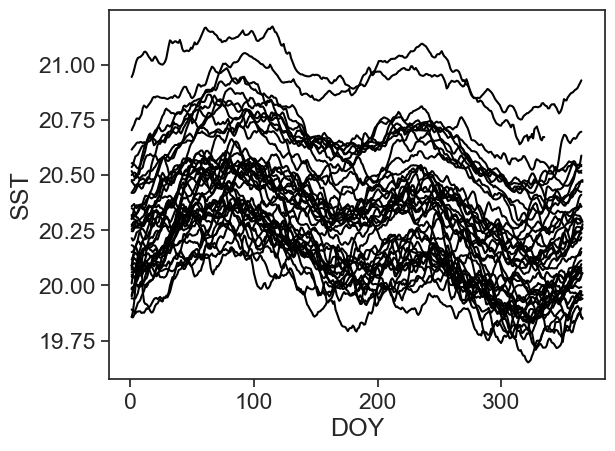
\includegraphics{resampling/resampling_files/figure-pdf/cell-11-output-1.png}

}

\end{figure}

Voilà! You made a beautiful graph!

\hypertarget{discussion-2}{%
\paragraph*{discussion}\label{discussion-2}}
\addcontentsline{toc}{paragraph}{discussion}

This time we did not put month numbers in the horizontal axis, we now
have month names. How did we do this black magic, you ask? See lines
8--10 above. Matplotlib gives you absolute power over what to put in the
axis, if you can only know how to tell it to\ldots{} Wanna know more?
\href{/best-practices/date-formatting.ipynb}{Click here.}

\hypertarget{upsampling}{%
\chapter{upsampling}\label{upsampling}}

In the previous chapter, we resampled from fine temporal resolution to a
coarser one. This is also called \textbf{downsampling}. We will learn
the \textbf{upsampling} now: how to go from coarse data to a finer
scale.

Sadly, there is no free lunch, and we just can't get data that was not
measured. What to do then?

It's best to consider a practical example.

\hypertarget{potential-evapotranspiration-using-penmans-equation}{%
\section{Potential Evapotranspiration using Penman's
equation}\label{potential-evapotranspiration-using-penmans-equation}}

We want to calculate the daily potential evapotranspiration using
\href{http://yairmau.com/surface-hydrology/evapotranspiration/evapotranspiration-lecture.html\#net-radiation}{Penman's
equation}. Part of the calculation involves characterizing the energy
budget on soil surface. When direct solar radiation measurements are not
available, we can estimate the energy balance by knowing the ``cloudless
skies mean solar radiation'', \(R_{so}\). This is the amount of energy
(MJ/m\(^2\)/d) that hits the surface, assuming no clouds. This radiation
depends on the season and on the latitude you are. For Israel, located
at latitude 32° N, we can use the following data for 30°:

\begin{Shaded}
\begin{Highlighting}[]
\ImportTok{import}\NormalTok{ numpy }\ImportTok{as}\NormalTok{ np}
\ImportTok{import}\NormalTok{ matplotlib.pyplot }\ImportTok{as}\NormalTok{ plt}
\ImportTok{import}\NormalTok{ pandas }\ImportTok{as}\NormalTok{ pd}
\ImportTok{from}\NormalTok{ matplotlib.dates }\ImportTok{import}\NormalTok{ DateFormatter}
\ImportTok{import}\NormalTok{ matplotlib.dates }\ImportTok{as}\NormalTok{ mdates}
\ImportTok{import}\NormalTok{ matplotlib.ticker }\ImportTok{as}\NormalTok{ ticker}
\ImportTok{import}\NormalTok{ seaborn }\ImportTok{as}\NormalTok{ sns}
\NormalTok{sns.}\BuiltInTok{set}\NormalTok{(style}\OperatorTok{=}\StringTok{"ticks"}\NormalTok{, font\_scale}\OperatorTok{=}\FloatTok{1.5}\NormalTok{)  }\CommentTok{\# white graphs, with large and legible letters}
\end{Highlighting}
\end{Shaded}

\begin{Shaded}
\begin{Highlighting}[]
\NormalTok{dates }\OperatorTok{=}\NormalTok{ pd.date\_range(start}\OperatorTok{=}\StringTok{\textquotesingle{}2021{-}01{-}01\textquotesingle{}}\NormalTok{, periods}\OperatorTok{=}\DecValTok{13}\NormalTok{, freq}\OperatorTok{=}\StringTok{\textquotesingle{}MS\textquotesingle{}}\NormalTok{)}
\NormalTok{values }\OperatorTok{=}\NormalTok{ [}\FloatTok{17.46}\NormalTok{, }\FloatTok{21.65}\NormalTok{, }\FloatTok{25.96}\NormalTok{, }\FloatTok{29.85}\NormalTok{, }\FloatTok{32.11}\NormalTok{, }\FloatTok{33.20}\NormalTok{, }\FloatTok{32.66}\NormalTok{, }\FloatTok{30.44}\NormalTok{, }\FloatTok{26.67}\NormalTok{, }\FloatTok{22.48}\NormalTok{, }\FloatTok{18.30}\NormalTok{, }\FloatTok{16.04}\NormalTok{, }\FloatTok{17.46}\NormalTok{]}
\NormalTok{df }\OperatorTok{=}\NormalTok{ pd.DataFrame(\{}\StringTok{\textquotesingle{}date\textquotesingle{}}\NormalTok{: dates, }\StringTok{\textquotesingle{}radiation\textquotesingle{}}\NormalTok{: values\})}
\NormalTok{df }\OperatorTok{=}\NormalTok{ df.set\_index(}\StringTok{\textquotesingle{}date\textquotesingle{}}\NormalTok{)}
\NormalTok{df}
\end{Highlighting}
\end{Shaded}

\begin{longtable}[]{@{}ll@{}}
\toprule\noalign{}
& radiation \\
date & \\
\midrule\noalign{}
\endhead
\bottomrule\noalign{}
\endlastfoot
2021-01-01 & 17.46 \\
2021-02-01 & 21.65 \\
2021-03-01 & 25.96 \\
2021-04-01 & 29.85 \\
2021-05-01 & 32.11 \\
2021-06-01 & 33.20 \\
2021-07-01 & 32.66 \\
2021-08-01 & 30.44 \\
2021-09-01 & 26.67 \\
2021-10-01 & 22.48 \\
2021-11-01 & 18.30 \\
2021-12-01 & 16.04 \\
2022-01-01 & 17.46 \\
\end{longtable}

\begin{Shaded}
\begin{Highlighting}[]
\NormalTok{fig, ax }\OperatorTok{=}\NormalTok{ plt.subplots()}
\NormalTok{ax.plot(df[}\StringTok{\textquotesingle{}radiation\textquotesingle{}}\NormalTok{], color}\OperatorTok{=}\StringTok{\textquotesingle{}black\textquotesingle{}}\NormalTok{, marker}\OperatorTok{=}\StringTok{\textquotesingle{}d\textquotesingle{}}\NormalTok{, linestyle}\OperatorTok{=}\StringTok{\textquotesingle{}None\textquotesingle{}}\NormalTok{)}
\NormalTok{ax.}\BuiltInTok{set}\NormalTok{(ylabel}\OperatorTok{=}\VerbatimStringTok{r\textquotesingle{}radiation (MJ/m$\^{}2$/d)\textquotesingle{}}\NormalTok{,}
\NormalTok{       title}\OperatorTok{=}\StringTok{"cloudless skies mean solar radiation for latitude 30° N"}\NormalTok{)}
\NormalTok{ax.xaxis.set\_major\_locator(mdates.MonthLocator())}
\NormalTok{date\_form }\OperatorTok{=}\NormalTok{ DateFormatter(}\StringTok{"\%b"}\NormalTok{)}
\NormalTok{ax.xaxis.set\_major\_formatter(date\_form)}
\NormalTok{plt.gcf().autofmt\_xdate()  }\CommentTok{\# makes slanted dates}
\end{Highlighting}
\end{Shaded}

\begin{figure}[H]

{\centering \includegraphics{resampling/upsampling_files/figure-pdf/cell-4-output-1.png}

}

\end{figure}

We only have 12 values for the whole year, and we can't use this
dataframe to compute daily ET. We need to upsample!

In the example below, we resample the monthly data into daily data, and
do nothing else. Pandas doesn't know what to do with the new points, so
it fills them with NaN.

\begin{Shaded}
\begin{Highlighting}[]
\NormalTok{df\_nan }\OperatorTok{=}\NormalTok{ df[}\StringTok{\textquotesingle{}radiation\textquotesingle{}}\NormalTok{].resample(}\StringTok{\textquotesingle{}D\textquotesingle{}}\NormalTok{).asfreq().to\_frame()}
\NormalTok{df\_nan.head(}\DecValTok{33}\NormalTok{)}
\end{Highlighting}
\end{Shaded}

\begin{longtable}[]{@{}ll@{}}
\toprule\noalign{}
& radiation \\
date & \\
\midrule\noalign{}
\endhead
\bottomrule\noalign{}
\endlastfoot
2021-01-01 & 17.46 \\
2021-01-02 & NaN \\
2021-01-03 & NaN \\
2021-01-04 & NaN \\
2021-01-05 & NaN \\
2021-01-06 & NaN \\
2021-01-07 & NaN \\
2021-01-08 & NaN \\
2021-01-09 & NaN \\
2021-01-10 & NaN \\
2021-01-11 & NaN \\
2021-01-12 & NaN \\
2021-01-13 & NaN \\
2021-01-14 & NaN \\
2021-01-15 & NaN \\
2021-01-16 & NaN \\
2021-01-17 & NaN \\
2021-01-18 & NaN \\
2021-01-19 & NaN \\
2021-01-20 & NaN \\
2021-01-21 & NaN \\
2021-01-22 & NaN \\
2021-01-23 & NaN \\
2021-01-24 & NaN \\
2021-01-25 & NaN \\
2021-01-26 & NaN \\
2021-01-27 & NaN \\
2021-01-28 & NaN \\
2021-01-29 & NaN \\
2021-01-30 & NaN \\
2021-01-31 & NaN \\
2021-02-01 & 21.65 \\
2021-02-02 & NaN \\
\end{longtable}

\hypertarget{forwardbackward-fill}{%
\section{Forward/Backward fill}\label{forwardbackward-fill}}

We can forward/backward fill these NaNs:

\begin{Shaded}
\begin{Highlighting}[]
\NormalTok{df\_forw }\OperatorTok{=}\NormalTok{ df[}\StringTok{\textquotesingle{}radiation\textquotesingle{}}\NormalTok{].resample(}\StringTok{\textquotesingle{}D\textquotesingle{}}\NormalTok{).ffill().to\_frame()}
\NormalTok{df\_back }\OperatorTok{=}\NormalTok{ df[}\StringTok{\textquotesingle{}radiation\textquotesingle{}}\NormalTok{].resample(}\StringTok{\textquotesingle{}D\textquotesingle{}}\NormalTok{).bfill().to\_frame()}
\end{Highlighting}
\end{Shaded}

\begin{Shaded}
\begin{Highlighting}[]
\NormalTok{fig, ax }\OperatorTok{=}\NormalTok{ plt.subplots()}
\NormalTok{ax.plot(df[}\StringTok{\textquotesingle{}radiation\textquotesingle{}}\NormalTok{], color}\OperatorTok{=}\StringTok{\textquotesingle{}black\textquotesingle{}}\NormalTok{, marker}\OperatorTok{=}\StringTok{\textquotesingle{}d\textquotesingle{}}\NormalTok{, linestyle}\OperatorTok{=}\StringTok{\textquotesingle{}None\textquotesingle{}}\NormalTok{, label}\OperatorTok{=}\StringTok{"original"}\NormalTok{)}
\NormalTok{ax.plot(df\_forw[}\StringTok{\textquotesingle{}radiation\textquotesingle{}}\NormalTok{], color}\OperatorTok{=}\StringTok{\textquotesingle{}tab:blue\textquotesingle{}}\NormalTok{, label}\OperatorTok{=}\StringTok{"forward fill"}\NormalTok{)}
\NormalTok{ax.plot(df\_back[}\StringTok{\textquotesingle{}radiation\textquotesingle{}}\NormalTok{], color}\OperatorTok{=}\StringTok{\textquotesingle{}tab:orange\textquotesingle{}}\NormalTok{, label}\OperatorTok{=}\StringTok{"backward fill"}\NormalTok{)}
\NormalTok{ax.}\BuiltInTok{set}\NormalTok{(ylabel}\OperatorTok{=}\VerbatimStringTok{r\textquotesingle{}radiation (MJ/m$\^{}2$/d)\textquotesingle{}}\NormalTok{,}
\NormalTok{       title}\OperatorTok{=}\StringTok{"cloudless skies mean solar radiation for latitude 30° N"}\NormalTok{)}
\NormalTok{ax.legend(frameon}\OperatorTok{=}\VariableTok{False}\NormalTok{, fontsize}\OperatorTok{=}\DecValTok{12}\NormalTok{)}
\NormalTok{ax.xaxis.set\_major\_locator(mdates.MonthLocator())}
\NormalTok{date\_form }\OperatorTok{=}\NormalTok{ DateFormatter(}\StringTok{"\%b"}\NormalTok{)}
\NormalTok{ax.xaxis.set\_major\_formatter(date\_form)}
\NormalTok{plt.gcf().autofmt\_xdate()  }\CommentTok{\# makes slanted dates}
\end{Highlighting}
\end{Shaded}

\begin{figure}[H]

{\centering \includegraphics{resampling/upsampling_files/figure-pdf/cell-7-output-1.png}

}

\end{figure}

This does the job, but I want something better, not step functions. The
radiation should vary smoothly from day to day. Let's use interpolation.

\hypertarget{interpolation}{%
\section{Interpolation}\label{interpolation}}

\begin{Shaded}
\begin{Highlighting}[]
\NormalTok{df\_linear }\OperatorTok{=}\NormalTok{ df[}\StringTok{\textquotesingle{}radiation\textquotesingle{}}\NormalTok{].resample(}\StringTok{\textquotesingle{}D\textquotesingle{}}\NormalTok{).interpolate(method}\OperatorTok{=}\StringTok{\textquotesingle{}time\textquotesingle{}}\NormalTok{).to\_frame()}
\NormalTok{df\_cubic }\OperatorTok{=}\NormalTok{ df[}\StringTok{\textquotesingle{}radiation\textquotesingle{}}\NormalTok{].resample(}\StringTok{\textquotesingle{}D\textquotesingle{}}\NormalTok{).interpolate(method}\OperatorTok{=}\StringTok{\textquotesingle{}cubic\textquotesingle{}}\NormalTok{).to\_frame()}
\end{Highlighting}
\end{Shaded}

\begin{Shaded}
\begin{Highlighting}[]
\NormalTok{fig, ax }\OperatorTok{=}\NormalTok{ plt.subplots()}
\NormalTok{ax.plot(df[}\StringTok{\textquotesingle{}radiation\textquotesingle{}}\NormalTok{], color}\OperatorTok{=}\StringTok{\textquotesingle{}black\textquotesingle{}}\NormalTok{, marker}\OperatorTok{=}\StringTok{\textquotesingle{}d\textquotesingle{}}\NormalTok{, linestyle}\OperatorTok{=}\StringTok{\textquotesingle{}None\textquotesingle{}}\NormalTok{, label}\OperatorTok{=}\StringTok{"original"}\NormalTok{)}
\NormalTok{ax.plot(df\_linear[}\StringTok{\textquotesingle{}radiation\textquotesingle{}}\NormalTok{], color}\OperatorTok{=}\StringTok{\textquotesingle{}tab:blue\textquotesingle{}}\NormalTok{, label}\OperatorTok{=}\StringTok{"linear interpolation"}\NormalTok{)}
\NormalTok{ax.plot(df\_cubic[}\StringTok{\textquotesingle{}radiation\textquotesingle{}}\NormalTok{], color}\OperatorTok{=}\StringTok{\textquotesingle{}tab:orange\textquotesingle{}}\NormalTok{, label}\OperatorTok{=}\StringTok{"cubic interpolation"}\NormalTok{)}
\NormalTok{ax.}\BuiltInTok{set}\NormalTok{(ylabel}\OperatorTok{=}\VerbatimStringTok{r\textquotesingle{}radiation (MJ/m$\^{}2$/d)\textquotesingle{}}\NormalTok{,}
\NormalTok{       title}\OperatorTok{=}\StringTok{"cloudless skies mean solar radiation for latitude 30° N"}\NormalTok{)}
\NormalTok{ax.legend(frameon}\OperatorTok{=}\VariableTok{False}\NormalTok{, fontsize}\OperatorTok{=}\DecValTok{12}\NormalTok{)}
\NormalTok{ax.xaxis.set\_major\_locator(mdates.MonthLocator())}
\NormalTok{date\_form }\OperatorTok{=}\NormalTok{ DateFormatter(}\StringTok{"\%b"}\NormalTok{)}
\NormalTok{ax.xaxis.set\_major\_formatter(date\_form)}
\NormalTok{plt.gcf().autofmt\_xdate()  }\CommentTok{\# makes slanted dates}
\end{Highlighting}
\end{Shaded}

\begin{figure}[H]

{\centering \includegraphics{resampling/upsampling_files/figure-pdf/cell-9-output-1.png}

}

\end{figure}

There are many ways to fill NaNs and to interpolate. A nice detailed
guide can be
\href{https://note.nkmk.me/en/python-pandas-interpolate/}{found here}.

\hypertarget{interpolation-1}{%
\chapter{interpolation}\label{interpolation-1}}

Interpolation is the act of getting data you don't have from data you
alreay have. We used some interpolation when upsampling, and now it is
time to talk about it a little bit more in depth.

There is no one correct way of interpolating, the method you use depends
in the end on what you want to accomplish, what are your (hidden or
explicit) assumptions, etc. Let's see a few examples.

\hypertarget{faq}{%
\chapter{FAQ}\label{faq}}

\hypertarget{how-to-resample-by-year-but-have-it-end-in-september}{%
\section{How to resample by year, but have it end in
September?}\label{how-to-resample-by-year-but-have-it-end-in-september}}

This is called
\href{https://pandas.pydata.org/pandas-docs/stable/user_guide/timeseries.html\#anchored-offsets}{anchored
offset}. One possible use to it is to calculate statistics according to
the hydrological year that, for example, ends in September.

\begin{Shaded}
\begin{Highlighting}[]
\ImportTok{import}\NormalTok{ numpy }\ImportTok{as}\NormalTok{ np}
\ImportTok{import}\NormalTok{ matplotlib.pyplot }\ImportTok{as}\NormalTok{ plt}
\ImportTok{import}\NormalTok{ pandas }\ImportTok{as}\NormalTok{ pd}
\ImportTok{from}\NormalTok{ matplotlib.dates }\ImportTok{import}\NormalTok{ DateFormatter}
\ImportTok{import}\NormalTok{ matplotlib.dates }\ImportTok{as}\NormalTok{ mdates}
\ImportTok{import}\NormalTok{ matplotlib.ticker }\ImportTok{as}\NormalTok{ ticker}
\ImportTok{import}\NormalTok{ seaborn }\ImportTok{as}\NormalTok{ sns}
\NormalTok{sns.}\BuiltInTok{set}\NormalTok{(style}\OperatorTok{=}\StringTok{"ticks"}\NormalTok{, font\_scale}\OperatorTok{=}\FloatTok{1.5}\NormalTok{)  }\CommentTok{\# white graphs, with large and legible letters}
\end{Highlighting}
\end{Shaded}

\begin{Shaded}
\begin{Highlighting}[]
\NormalTok{filename }\OperatorTok{=} \StringTok{"../archive/data/Kinneret\_Kvuza\_daily\_rainfall.csv"}
\NormalTok{df }\OperatorTok{=}\NormalTok{ pd.read\_csv(filename, na\_values}\OperatorTok{=}\NormalTok{[}\StringTok{\textquotesingle{}{-}\textquotesingle{}}\NormalTok{])}
\NormalTok{df.rename(columns}\OperatorTok{=}\NormalTok{\{}\StringTok{\textquotesingle{}Date\textquotesingle{}}\NormalTok{: }\StringTok{\textquotesingle{}date\textquotesingle{}}\NormalTok{,}
                   \StringTok{\textquotesingle{}Daily Rainfall (mm)\textquotesingle{}}\NormalTok{: }\StringTok{\textquotesingle{}rain\textquotesingle{}}\NormalTok{\}, inplace}\OperatorTok{=}\VariableTok{True}\NormalTok{)}
\NormalTok{df[}\StringTok{\textquotesingle{}date\textquotesingle{}}\NormalTok{] }\OperatorTok{=}\NormalTok{ pd.to\_datetime(df[}\StringTok{\textquotesingle{}date\textquotesingle{}}\NormalTok{], dayfirst}\OperatorTok{=}\VariableTok{True}\NormalTok{)}
\NormalTok{df }\OperatorTok{=}\NormalTok{ df.set\_index(}\StringTok{\textquotesingle{}date\textquotesingle{}}\NormalTok{)}
\NormalTok{df }\OperatorTok{=}\NormalTok{ df.resample(}\StringTok{\textquotesingle{}D\textquotesingle{}}\NormalTok{).asfreq().fillna(}\DecValTok{0}\NormalTok{)  }\CommentTok{\# asfreq = replace}
\NormalTok{df}
\end{Highlighting}
\end{Shaded}

\begin{longtable}[]{@{}lll@{}}
\toprule\noalign{}
& Station & rain \\
date & & \\
\midrule\noalign{}
\endhead
\bottomrule\noalign{}
\endlastfoot
1980-01-02 & Kinneret Kvuza 09/1977-08/2023 & 0.0 \\
1980-01-03 & 0 & 0.0 \\
1980-01-04 & 0 & 0.0 \\
1980-01-05 & Kinneret Kvuza 09/1977-08/2023 & 35.5 \\
1980-01-06 & Kinneret Kvuza 09/1977-08/2023 & 2.2 \\
... & ... & ... \\
2019-12-26 & Kinneret Kvuza 09/1977-08/2023 & 39.4 \\
2019-12-27 & Kinneret Kvuza 09/1977-08/2023 & 5.2 \\
2019-12-28 & Kinneret Kvuza 09/1977-08/2023 & 1.6 \\
2019-12-29 & 0 & 0.0 \\
2019-12-30 & Kinneret Kvuza 09/1977-08/2023 & 0.1 \\
\end{longtable}

\begin{Shaded}
\begin{Highlighting}[]
\NormalTok{fig, ax }\OperatorTok{=}\NormalTok{ plt.subplots(}\DecValTok{2}\NormalTok{,}\DecValTok{1}\NormalTok{)}
\NormalTok{ax[}\DecValTok{0}\NormalTok{].plot(df[}\StringTok{\textquotesingle{}rain\textquotesingle{}}\NormalTok{], color}\OperatorTok{=}\StringTok{\textquotesingle{}black\textquotesingle{}}\NormalTok{)}
\NormalTok{ax[}\DecValTok{1}\NormalTok{].plot(df.loc[}\StringTok{\textquotesingle{}1998\textquotesingle{}}\NormalTok{:}\StringTok{\textquotesingle{}2000\textquotesingle{}}\NormalTok{, }\StringTok{\textquotesingle{}rain\textquotesingle{}}\NormalTok{], color}\OperatorTok{=}\StringTok{\textquotesingle{}black\textquotesingle{}}\NormalTok{)}
\NormalTok{locator }\OperatorTok{=}\NormalTok{ mdates.AutoDateLocator(minticks}\OperatorTok{=}\DecValTok{4}\NormalTok{, maxticks}\OperatorTok{=}\DecValTok{8}\NormalTok{)}
\NormalTok{formatter }\OperatorTok{=}\NormalTok{ mdates.ConciseDateFormatter(locator)}
\NormalTok{ax[}\DecValTok{1}\NormalTok{].xaxis.set\_major\_locator(locator)}
\NormalTok{ax[}\DecValTok{1}\NormalTok{].xaxis.set\_major\_formatter(formatter)}
\NormalTok{fig.text(}\FloatTok{0.02}\NormalTok{, }\FloatTok{0.5}\NormalTok{, }\StringTok{\textquotesingle{}daily precipitation (mm)\textquotesingle{}}\NormalTok{, va}\OperatorTok{=}\StringTok{\textquotesingle{}center\textquotesingle{}}\NormalTok{, rotation}\OperatorTok{=}\StringTok{\textquotesingle{}vertical\textquotesingle{}}\NormalTok{)}
\NormalTok{ax[}\DecValTok{0}\NormalTok{].set\_title(}\StringTok{"Kvutzat Kinneret"}\NormalTok{)}
\end{Highlighting}
\end{Shaded}

\begin{verbatim}
Text(0.5, 1.0, 'Kvutzat Kinneret')
\end{verbatim}

\begin{figure}[H]

{\centering 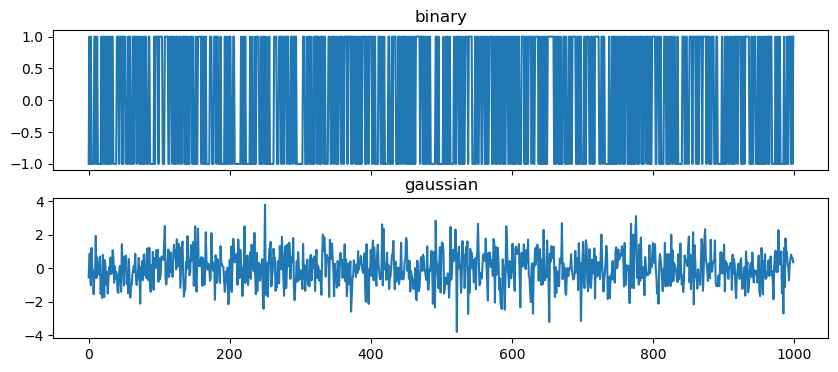
\includegraphics{resampling/FAQ_files/figure-pdf/cell-4-output-2.png}

}

\end{figure}

We see a marked dry season during the summer, so let's assume the
Hydrological Year ends in September.

\begin{Shaded}
\begin{Highlighting}[]
\NormalTok{df\_year }\OperatorTok{=}\NormalTok{ df.resample(}\StringTok{\textquotesingle{}A{-}SEP\textquotesingle{}}\NormalTok{).}\BuiltInTok{sum}\NormalTok{()}
\NormalTok{df\_year }\OperatorTok{=}\NormalTok{ df\_year.loc[}\StringTok{\textquotesingle{}1980\textquotesingle{}}\NormalTok{:}\StringTok{\textquotesingle{}2003\textquotesingle{}}\NormalTok{]}
\NormalTok{df\_year}
\end{Highlighting}
\end{Shaded}

\begin{verbatim}
/var/folders/c3/7hp0d36n6vv8jc9hm2440__00000gn/T/ipykernel_94063/2047090134.py:1: FutureWarning: The default value of numeric_only in DataFrameGroupBy.sum is deprecated. In a future version, numeric_only will default to False. Either specify numeric_only or select only columns which should be valid for the function.
  df_year = df.resample('A-SEP').sum()
\end{verbatim}

\begin{longtable}[]{@{}ll@{}}
\toprule\noalign{}
& rain \\
date & \\
\midrule\noalign{}
\endhead
\bottomrule\noalign{}
\endlastfoot
1980-09-30 & 355.5 \\
1981-09-30 & 463.1 \\
1982-09-30 & 221.7 \\
1983-09-30 & 557.1 \\
1984-09-30 & 335.3 \\
1985-09-30 & 379.8 \\
1986-09-30 & 300.7 \\
1987-09-30 & 424.7 \\
1988-09-30 & 421.6 \\
1989-09-30 & 251.6 \\
1990-09-30 & 432.5 \\
1991-09-30 & 328.3 \\
1992-09-30 & 738.4 \\
1993-09-30 & 434.9 \\
1994-09-30 & 255.4 \\
1995-09-30 & 408.6 \\
1996-09-30 & 373.0 \\
1997-09-30 & 416.2 \\
1998-09-30 & 451.9 \\
1999-09-30 & 227.8 \\
2000-09-30 & 378.9 \\
2001-09-30 & 273.9 \\
2002-09-30 & 445.2 \\
2003-09-30 & 602.4 \\
\end{longtable}

\begin{Shaded}
\begin{Highlighting}[]
\NormalTok{fig, ax }\OperatorTok{=}\NormalTok{ plt.subplots()}
\NormalTok{ax.bar(df\_year.index, df\_year[}\StringTok{\textquotesingle{}rain\textquotesingle{}}\NormalTok{], color}\OperatorTok{=}\StringTok{\textquotesingle{}black\textquotesingle{}}\NormalTok{,}
\NormalTok{       width}\OperatorTok{=}\DecValTok{365}\NormalTok{)}
\NormalTok{ax.set\_ylabel(}\StringTok{"yearly precipitation (mm)"}\NormalTok{)}
\NormalTok{ax.set\_title(}\StringTok{"Kvutzat Kinneret"}\NormalTok{)}
\end{Highlighting}
\end{Shaded}

\begin{verbatim}
Text(0.5, 1.0, 'Kvutzat Kinneret')
\end{verbatim}

\begin{figure}[H]

{\centering \includegraphics{resampling/FAQ_files/figure-pdf/cell-6-output-2.png}

}

\end{figure}

\hypertarget{when-upsampling-how-to-fill-missing-values-with-zero}{%
\section{When upsampling, how to fill missing values with
zero?}\label{when-upsampling-how-to-fill-missing-values-with-zero}}

We did that in the example above, like this:

\begin{Shaded}
\begin{Highlighting}[]
\NormalTok{df }\OperatorTok{=}\NormalTok{ df.resample(}\StringTok{\textquotesingle{}D\textquotesingle{}}\NormalTok{).asfreq().fillna(}\DecValTok{0}\NormalTok{)  }\CommentTok{\# asfreq = replace}
\end{Highlighting}
\end{Shaded}

\part{smoothing}

\hypertarget{motivation-1}{%
\chapter{motivation}\label{motivation-1}}

This is the temperature for the Yatir Forest (Shani station, see
\href{https://maps.app.goo.gl/JXfHcjE2Vn8YbS91A}{map}), between 2 and 5
of January 2022. Data is in intervals of 10 minutes, and was downloaded
from the Israel Meteorological Service.

\begin{Shaded}
\begin{Highlighting}[]
\ImportTok{import}\NormalTok{ numpy }\ImportTok{as}\NormalTok{ np}
\ImportTok{import}\NormalTok{ matplotlib.pyplot }\ImportTok{as}\NormalTok{ plt}
\ImportTok{import}\NormalTok{ pandas }\ImportTok{as}\NormalTok{ pd}
\ImportTok{from}\NormalTok{ matplotlib.dates }\ImportTok{import}\NormalTok{ DateFormatter}
\ImportTok{import}\NormalTok{ matplotlib.dates }\ImportTok{as}\NormalTok{ mdates}
\ImportTok{import}\NormalTok{ datetime }\ImportTok{as}\NormalTok{ dt}
\ImportTok{import}\NormalTok{ matplotlib.ticker }\ImportTok{as}\NormalTok{ ticker}
\ImportTok{import}\NormalTok{ warnings}
\CommentTok{\# Suppress FutureWarnings}
\NormalTok{warnings.simplefilter(action}\OperatorTok{=}\StringTok{\textquotesingle{}ignore\textquotesingle{}}\NormalTok{, category}\OperatorTok{=}\PreprocessorTok{FutureWarning}\NormalTok{)}
\ImportTok{import}\NormalTok{ seaborn }\ImportTok{as}\NormalTok{ sns}
\NormalTok{sns.}\BuiltInTok{set}\NormalTok{(style}\OperatorTok{=}\StringTok{"ticks"}\NormalTok{, font\_scale}\OperatorTok{=}\FloatTok{1.5}\NormalTok{)  }\CommentTok{\# white graphs, with large and legible letters}
\ImportTok{import}\NormalTok{ requests}
\ImportTok{import}\NormalTok{ json}
\CommentTok{\# \%matplotlib widget}
\end{Highlighting}
\end{Shaded}

\begin{Shaded}
\begin{Highlighting}[]
\CommentTok{\# useful links}
\CommentTok{\# https://ims.gov.il/he/ObservationDataAPI}
\CommentTok{\# https://ims.gov.il/sites/default/files/2021{-}09/API\%20explanation.pdf}
\CommentTok{\# https://ims.gov.il/sites/default/files/2022{-}04/Python\%20API\%20example.pdf}

\ControlFlowTok{with} \BuiltInTok{open}\NormalTok{(}\StringTok{\textquotesingle{}IMS{-}token.txt\textquotesingle{}}\NormalTok{, }\StringTok{\textquotesingle{}r\textquotesingle{}}\NormalTok{) }\ImportTok{as} \BuiltInTok{file}\NormalTok{:}
\NormalTok{    TOKEN }\OperatorTok{=} \BuiltInTok{file}\NormalTok{.readline()}
\NormalTok{STATION\_NUM }\OperatorTok{=} \DecValTok{28}  \CommentTok{\# 28 = "SHANI"}
\NormalTok{DATA }\OperatorTok{=} \DecValTok{10}  \CommentTok{\# 10 = TDmax (max temperature)}
\NormalTok{start }\OperatorTok{=} \StringTok{"2022/01/01"}
\NormalTok{end }\OperatorTok{=} \StringTok{"2022/02/01"}
\NormalTok{url }\OperatorTok{=} \SpecialStringTok{f"https://api.ims.gov.il/v1/envista/stations/}\SpecialCharTok{\{}\NormalTok{STATION\_NUM}\SpecialCharTok{\}}\SpecialStringTok{/data/}\SpecialCharTok{\{}\NormalTok{DATA}\SpecialCharTok{\}}\SpecialStringTok{/?from=}\SpecialCharTok{\{}\NormalTok{start}\SpecialCharTok{\}}\SpecialStringTok{\&to=}\SpecialCharTok{\{}\NormalTok{end}\SpecialCharTok{\}}\SpecialStringTok{"}
\NormalTok{headers }\OperatorTok{=}\NormalTok{ \{}\StringTok{\textquotesingle{}Authorization\textquotesingle{}}\NormalTok{: }\SpecialStringTok{f\textquotesingle{}ApiToken }\SpecialCharTok{\{}\NormalTok{TOKEN}\SpecialCharTok{\}}\SpecialStringTok{\textquotesingle{}}\NormalTok{\}}
\NormalTok{response }\OperatorTok{=}\NormalTok{ requests.request(}\StringTok{"GET"}\NormalTok{, url, headers}\OperatorTok{=}\NormalTok{headers)}
\NormalTok{data}\OperatorTok{=}\NormalTok{ json.loads(response.text.encode(}\StringTok{\textquotesingle{}utf8\textquotesingle{}}\NormalTok{))}
\end{Highlighting}
\end{Shaded}

\begin{Shaded}
\begin{Highlighting}[]
\NormalTok{df }\OperatorTok{=}\NormalTok{ pd.json\_normalize(data[}\StringTok{\textquotesingle{}data\textquotesingle{}}\NormalTok{],record\_path}\OperatorTok{=}\NormalTok{[}\StringTok{\textquotesingle{}channels\textquotesingle{}}\NormalTok{], meta}\OperatorTok{=}\NormalTok{[}\StringTok{\textquotesingle{}datetime\textquotesingle{}}\NormalTok{])}
\NormalTok{df[}\StringTok{\textquotesingle{}date\textquotesingle{}}\NormalTok{] }\OperatorTok{=}\NormalTok{ pd.to\_datetime(df[}\StringTok{\textquotesingle{}datetime\textquotesingle{}}\NormalTok{])}
\NormalTok{df }\OperatorTok{=}\NormalTok{ df.set\_index(}\StringTok{\textquotesingle{}date\textquotesingle{}}\NormalTok{)}
\CommentTok{\# df}
\end{Highlighting}
\end{Shaded}

\begin{Shaded}
\begin{Highlighting}[]
\CommentTok{\# dirty trick to have dates in the middle of the 24{-}hour period}
\CommentTok{\# make minor ticks in the middle, put the labels there!}
\CommentTok{\# from https://matplotlib.org/stable/gallery/ticks/centered\_ticklabels.html}

\KeywordTok{def}\NormalTok{ centered\_dates(ax):}
\NormalTok{    date\_form }\OperatorTok{=}\NormalTok{ DateFormatter(}\StringTok{"}\SpecialCharTok{\%d}\StringTok{ \%b"}\NormalTok{)  }\CommentTok{\# \%d 3{-}letter{-}Month}
    \CommentTok{\# major ticks at midnight, every day}
\NormalTok{    ax.xaxis.set\_major\_locator(mdates.DayLocator(interval}\OperatorTok{=}\DecValTok{1}\NormalTok{))}
\NormalTok{    ax.xaxis.set\_major\_formatter(date\_form)}
    \CommentTok{\# minor ticks at noon, every day}
\NormalTok{    ax.xaxis.set\_minor\_locator(mdates.HourLocator(byhour}\OperatorTok{=}\NormalTok{[}\DecValTok{12}\NormalTok{]))}
    \CommentTok{\# erase major tick labels}
\NormalTok{    ax.xaxis.set\_major\_formatter(ticker.NullFormatter())}
    \CommentTok{\# set minor tick labels as define above}
\NormalTok{    ax.xaxis.set\_minor\_formatter(date\_form)}
    \CommentTok{\# completely erase minor ticks, center tick labels}
    \ControlFlowTok{for}\NormalTok{ tick }\KeywordTok{in}\NormalTok{ ax.xaxis.get\_minor\_ticks():}
\NormalTok{        tick.tick1line.set\_markersize(}\DecValTok{0}\NormalTok{)}
\NormalTok{        tick.tick2line.set\_markersize(}\DecValTok{0}\NormalTok{)}
\NormalTok{        tick.label1.set\_horizontalalignment(}\StringTok{\textquotesingle{}center\textquotesingle{}}\NormalTok{)}
\end{Highlighting}
\end{Shaded}

\begin{Shaded}
\begin{Highlighting}[]
\NormalTok{fig, ax }\OperatorTok{=}\NormalTok{ plt.subplots(figsize}\OperatorTok{=}\NormalTok{(}\DecValTok{8}\NormalTok{,}\DecValTok{5}\NormalTok{))}
\NormalTok{start }\OperatorTok{=} \StringTok{"2022{-}01{-}02"}
\NormalTok{end }\OperatorTok{=} \StringTok{"2022{-}01{-}05"}
\NormalTok{df }\OperatorTok{=}\NormalTok{ df.loc[start:end]}
\NormalTok{ax.plot(df[}\StringTok{\textquotesingle{}value\textquotesingle{}}\NormalTok{], color}\OperatorTok{=}\StringTok{\textquotesingle{}black\textquotesingle{}}\NormalTok{)}
\NormalTok{ax.}\BuiltInTok{set}\NormalTok{(ylim}\OperatorTok{=}\NormalTok{[}\DecValTok{5}\NormalTok{, }\FloatTok{17.5}\NormalTok{],}
\NormalTok{       xlim}\OperatorTok{=}\NormalTok{[df.index[}\DecValTok{0}\NormalTok{], df.index[}\OperatorTok{{-}}\DecValTok{1}\NormalTok{]],}
\NormalTok{       ylabel}\OperatorTok{=}\StringTok{"Temperature (°C)"}\NormalTok{,}
\NormalTok{       title}\OperatorTok{=}\StringTok{"Yatir Forest, 2022"}\NormalTok{,}
\NormalTok{       yticks}\OperatorTok{=}\NormalTok{[}\DecValTok{5}\NormalTok{,}\DecValTok{10}\NormalTok{,}\DecValTok{15}\NormalTok{])}
\NormalTok{centered\_dates(ax)}
\end{Highlighting}
\end{Shaded}

\begin{figure}[H]

{\centering \includegraphics{smoothing/motivation_files/figure-pdf/cell-6-output-1.png}

}

\end{figure}

We see that the temperature curve has a rough profile. Can we find ways
of getting smoother curves?

We learned how to average over a window with \texttt{resample}. Let's
try that for a 2-hour window:

\begin{Shaded}
\begin{Highlighting}[]
\NormalTok{fig, ax }\OperatorTok{=}\NormalTok{ plt.subplots(figsize}\OperatorTok{=}\NormalTok{(}\DecValTok{8}\NormalTok{,}\DecValTok{5}\NormalTok{))}
\NormalTok{ax.plot(df[}\StringTok{\textquotesingle{}value\textquotesingle{}}\NormalTok{], color}\OperatorTok{=}\StringTok{\textquotesingle{}black\textquotesingle{}}\NormalTok{)}
\NormalTok{ax.plot(df[}\StringTok{\textquotesingle{}value\textquotesingle{}}\NormalTok{].resample(}\StringTok{\textquotesingle{}2H\textquotesingle{}}\NormalTok{).mean(),}
\NormalTok{        color}\OperatorTok{=}\StringTok{\textquotesingle{}xkcd:hot pink\textquotesingle{}}\NormalTok{, ls}\OperatorTok{=}\StringTok{\textquotesingle{}{-}\textquotesingle{}}\NormalTok{,}
\NormalTok{        marker}\OperatorTok{=}\StringTok{"o"}\NormalTok{, mfc}\OperatorTok{=}\StringTok{"None"}\NormalTok{)}
\NormalTok{ax.}\BuiltInTok{set}\NormalTok{(ylim}\OperatorTok{=}\NormalTok{[}\DecValTok{5}\NormalTok{, }\FloatTok{17.5}\NormalTok{],}
\NormalTok{       xlim}\OperatorTok{=}\NormalTok{[df.index[}\DecValTok{0}\NormalTok{], df.index[}\OperatorTok{{-}}\DecValTok{1}\NormalTok{]],}
\NormalTok{       ylabel}\OperatorTok{=}\StringTok{"Temperature (°C)"}\NormalTok{,}
\NormalTok{       title}\OperatorTok{=}\StringTok{"Yatir Forest, 2022"}\NormalTok{,}
\NormalTok{       yticks}\OperatorTok{=}\NormalTok{[}\DecValTok{5}\NormalTok{,}\DecValTok{10}\NormalTok{,}\DecValTok{15}\NormalTok{])}
\NormalTok{centered\_dates(ax)}
\end{Highlighting}
\end{Shaded}

\begin{figure}[H]

{\centering \includegraphics{smoothing/motivation_files/figure-pdf/cell-7-output-1.png}

}

\end{figure}

The temperature profile now is much smoother, but when using
\texttt{resample}, we lost temporal resolution. Our original data had
10-minute frequency, and now we have a 2-hour frequency.

How can we get a smoother curve without losing resolution?

\hypertarget{tumbling-vs-sliding}{%
\section{Tumbling vs Sliding}\label{tumbling-vs-sliding}}

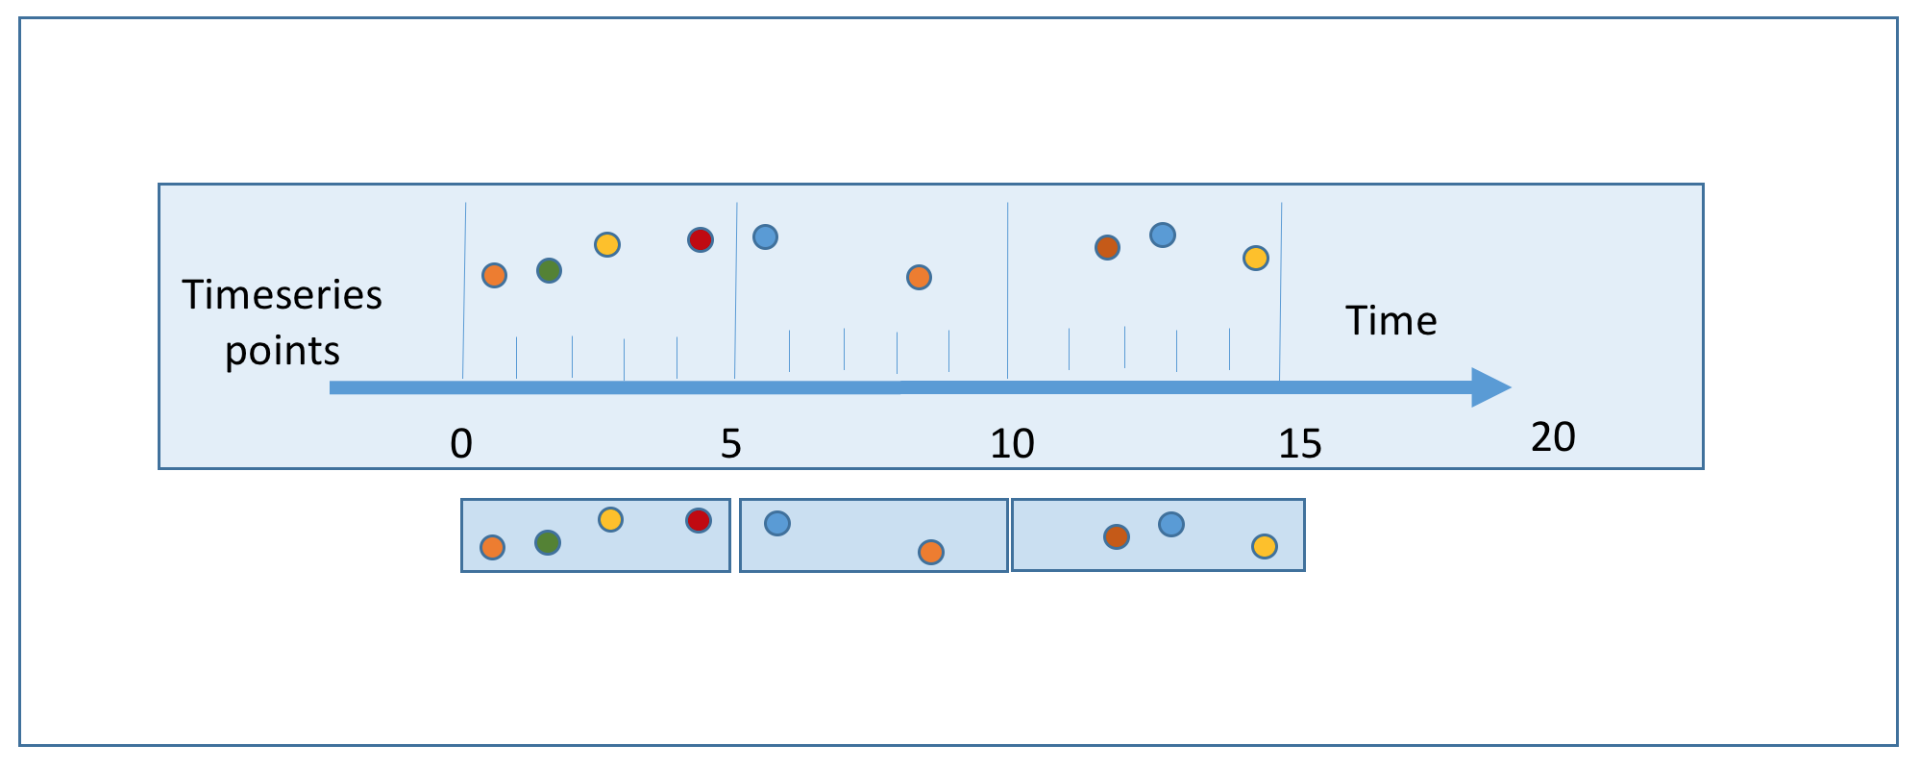
\includegraphics{smoothing/5sec_tumbling_window.png}
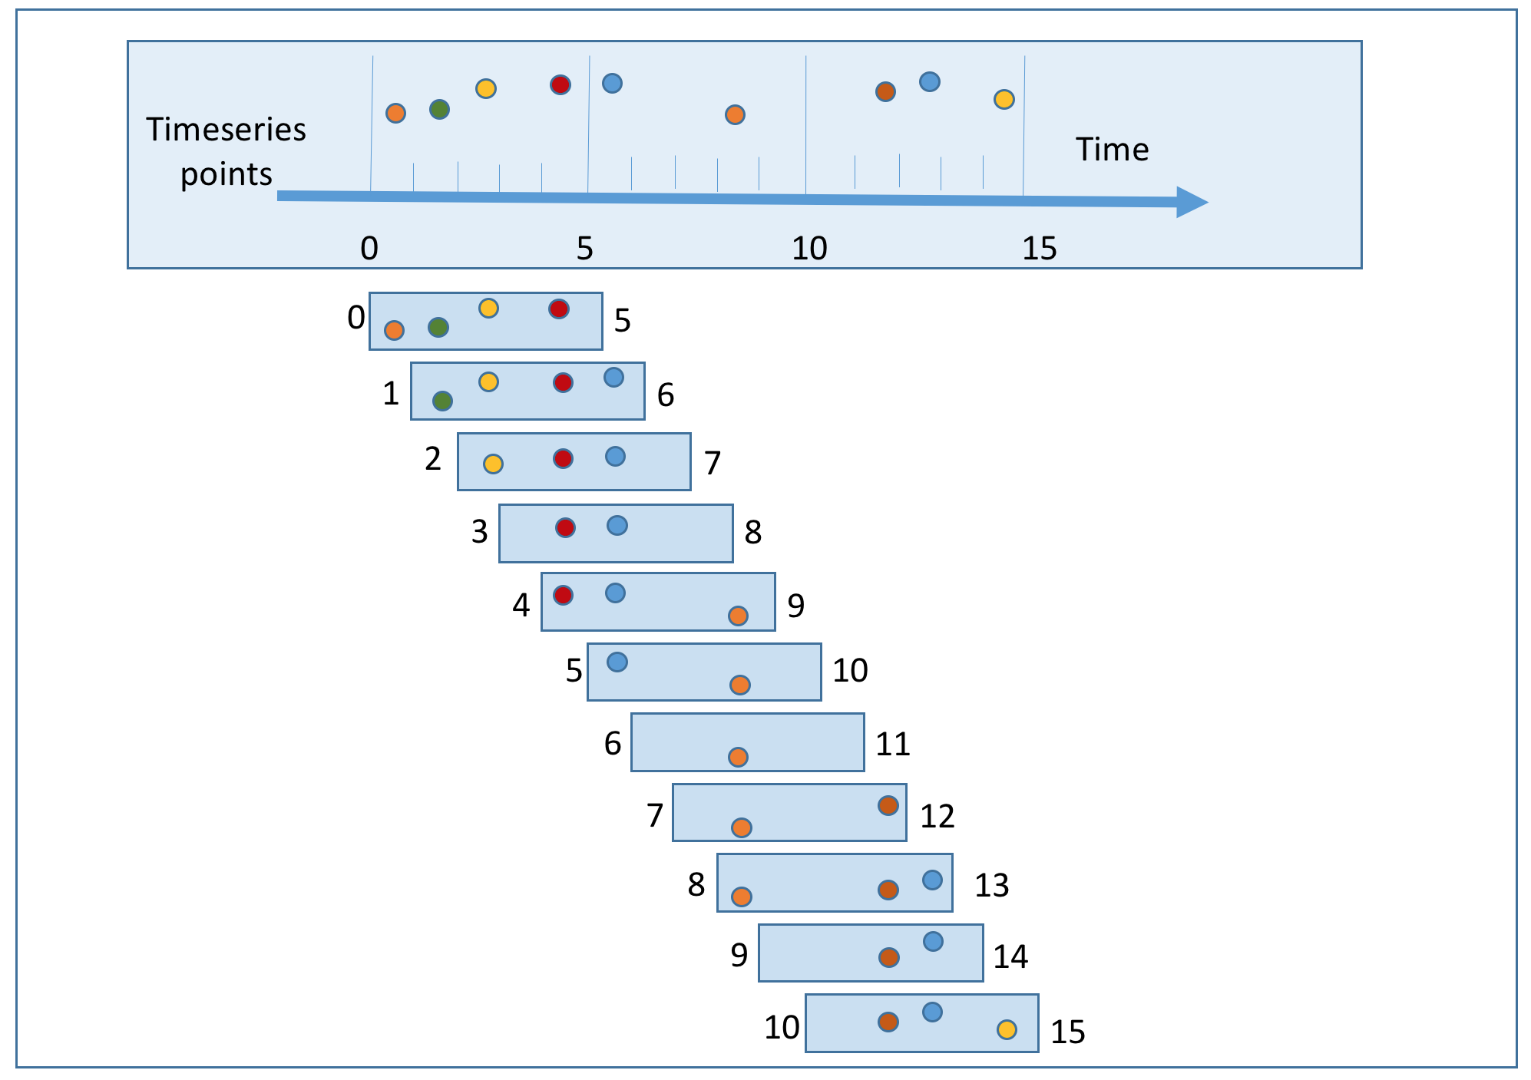
\includegraphics{smoothing/5sec_moving_window.png}

\hypertarget{sliding-window}{%
\chapter{sliding window}\label{sliding-window}}

Sliding windows of different shapes (kernels)

\hfill\break

This is the temperature for the Yatir Forest, between 2 and 5 of January
2022. Data is in intervals of 10 minutes, and was downloaded from the
Israel Meteorological Service.

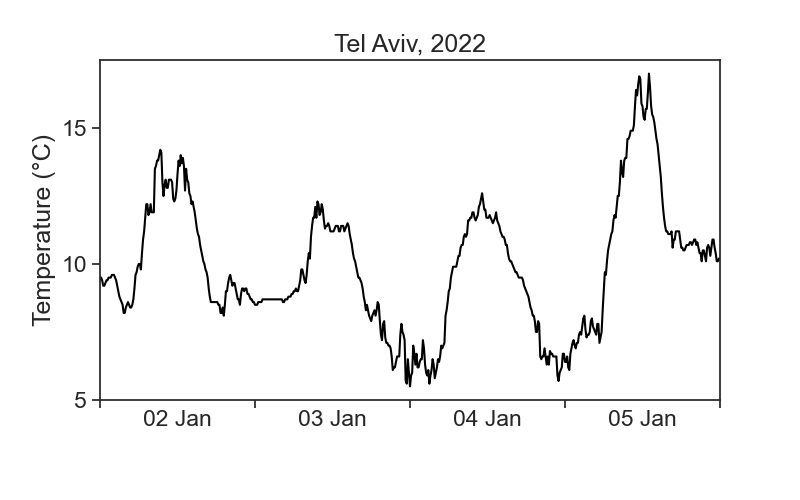
\includegraphics{smoothing/convolution_TA_temperature_2022.png}

We see that the temperature curve has a rough profile. Can we find ways
of getting smoother curves?

\hypertarget{convolution}{%
\section{convolution}\label{convolution}}

Convolution is a fancy word for averaging a time series using a sliding
window. We will use the terms \textbf{convolution, running average, and
rolling average} interchangeably. See the animation below. We take all
temperature values inside a window of width 500 minutes (51 points), and
average them with equal weights. The weights profile is called
\texttt{kernel}.

The pink curve is much smoother than the original! However, the running
average cannot describe sharp temperature changes. If we decrease the
window width to 200 minutes (21 points), we get the following result.

There is a tradeoff between the smoothness of a curve, and its ability
to describe sharp temporal changes.

\hypertarget{kernels}{%
\section{kernels}\label{kernels}}

We can modify our running average, so that values closer to the center
of the window have higher weights, and those further away count less.
This is achieved by changing the weight profile, or the shape of the
kernel. We see below the result of a running average using a triangular
window of base 500 minutes (51 points).

Things can get as fancy as we want. Instead of a triangular kernel,
which has sharp edges, we can choose a smoother gaussian kernel, see the
difference below. We used a gaussian kernel with 60-minute standard
deviation (the window in the animation is 4 standard deviations wide).

\hypertarget{math}{%
\section{math}\label{math}}

The definition of a convolution between signal \(f(t)\) and kernel
\(k(t)\) is

\[
(f * k)(t) = \int f(\tau)k(t-\tau)d\tau.
\]

The expression \(f*k\) denotes the convolution of these two functions.
The argument of \(k\) is \(t-\tau\), meaning that the kernel runs from
left to right (as \(t\) does), and at every point the two signals (\(f\)
and \(k\)) are multiplied together. It is the product of the signal with
the weight function \(k\) that gives us an average. Because of
\(-\tau\), the kernel is flipped backwards, but this has no effect to
symmetric kernels, like to ones in the examples above. Finally, the
actual running average is not the convolution, but

\[
\frac{(f * k)(t)}{\displaystyle \int k(t)dt}.
\]

Whenever the integral of the kernel is 1, then the convolution will be
identical with the running average.

\hypertarget{numerics}{%
\section{numerics}\label{numerics}}

Running averages are very common tools in time-series analysis. The
\texttt{pandas} package makes life quite simple. For example, in order
to calculate the running average of temperature using a rectangular
kernel, one writes

\begin{Shaded}
\begin{Highlighting}[]
\NormalTok{df[}\StringTok{\textquotesingle{}temperature\textquotesingle{}}\NormalTok{].rolling(window}\OperatorTok{=}\StringTok{\textquotesingle{}20\textquotesingle{}}\NormalTok{, center}\OperatorTok{=}\VariableTok{True}\NormalTok{).mean()}
\end{Highlighting}
\end{Shaded}

\begin{itemize}
\tightlist
\item
  \texttt{window=20} means that the width of the window is 20 points.
  Pandas lets us define a window width in time units, for example,
  \texttt{window=\textquotesingle{}120min\textquotesingle{}}.
\item
  \texttt{center=True} is needed in order to assign the result of
  averaging to the center of the window. Make it \texttt{False} and see
  what happens.
\item
  \texttt{mean()} is the actual calculation, the average of temperature
  over the window. The \texttt{rolling} part does not compute anything,
  it just creates a moving window, and we are free to calculate whatever
  we want. Try to calculate the standard deviation or the maximum, for
  example.
\end{itemize}

It is implicit in the command above a ``rectangular'' kernel. What if we
want other shapes?

\hypertarget{gaussian}{%
\subsection{gaussian}\label{gaussian}}

\begin{Shaded}
\begin{Highlighting}[]
\NormalTok{(}
\NormalTok{df[}\StringTok{\textquotesingle{}temperature\textquotesingle{}}\NormalTok{].rolling(window}\OperatorTok{=}\NormalTok{window\_width,}
\NormalTok{                          center}\OperatorTok{=}\VariableTok{True}\NormalTok{,}
\NormalTok{                          win\_type}\OperatorTok{=}\StringTok{"gaussian"}\NormalTok{)}
\NormalTok{                 .mean(std}\OperatorTok{=}\NormalTok{std\_gaussian)}
\NormalTok{)}
\end{Highlighting}
\end{Shaded}

where

\begin{itemize}
\tightlist
\item
  \texttt{window\_width} is an integer, number of points in your window
\item
  \texttt{std\_gaussian} is the standard deviation of your gaussian,
  measured in sample points, not time!
\end{itemize}

For instance, if we have measurements every 10 minutes, and our window
width is 500 minutes, then \texttt{window\_width\ =\ 500/10\ +\ 1}
(first and last included). If we want a standard deviation of 60
minutes, then \texttt{std\_gaussian\ =\ 6}. The gaussian kernel will
look like this:

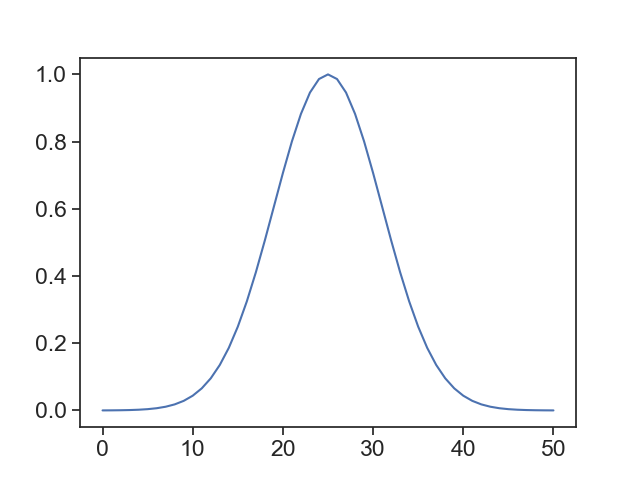
\includegraphics{smoothing/gaussian_kernel.png}

You can take a look at various options for kernel shapes
\href{https://docs.scipy.org/doc/scipy/reference/signal.windows.html\#module-scipy.signal.windows}{here},
provided by the \texttt{scipy} package. The graph above was achieved by
running:

\begin{Shaded}
\begin{Highlighting}[]
\NormalTok{g }\OperatorTok{=}\NormalTok{ scipy.signal.gaussian(window\_width, std)}
\NormalTok{plt.plot(g)}
\end{Highlighting}
\end{Shaded}

\hypertarget{triangular}{%
\subsection{triangular}\label{triangular}}

Same idea as gaussian, but simpler, because we don't need to think about
standard deviation.

\begin{Shaded}
\begin{Highlighting}[]
\NormalTok{(}
\NormalTok{df[}\StringTok{\textquotesingle{}temperature\textquotesingle{}}\NormalTok{].rolling(window}\OperatorTok{=}\NormalTok{window\_width,}
\NormalTok{                          center}\OperatorTok{=}\VariableTok{True}\NormalTok{,}
\NormalTok{                          win\_type}\OperatorTok{=}\StringTok{"triang"}\NormalTok{)}
\NormalTok{                 .mean()}
\NormalTok{)}
\end{Highlighting}
\end{Shaded}

\hypertarget{which-window-shape-and-width-to-choose}{%
\section{which window shape and width to
choose?}\label{which-window-shape-and-width-to-choose}}

🤷‍♂️

Sorry, there is not definite answer here\ldots{} It really depends on
your data and what you need to do with it. See below a comparison of all
examples in the videos above.

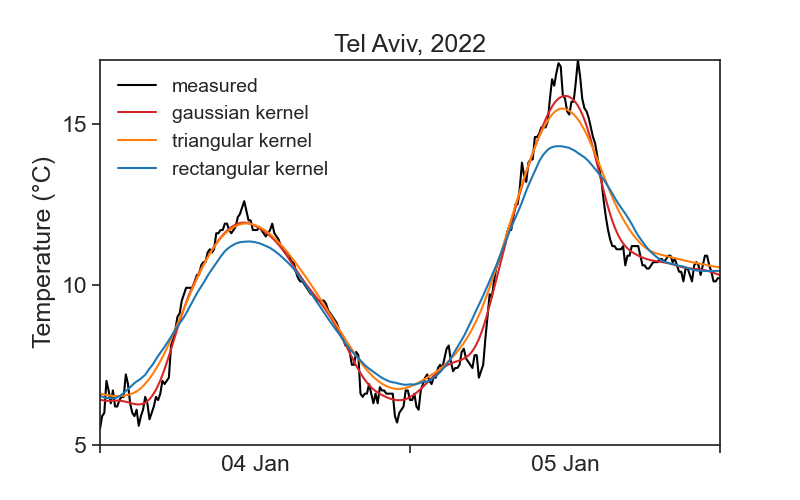
\includegraphics{smoothing/kernel_comparison.png}

One important question you need to ask is: what are the time scales
associated with the processes I'm interested in? For example, if I'm
interested in the daily temperature pattern, getting rid of
1-minute-long fluctuations would probably be ok. On the other hand, if
we were to smooth the signal so much that all that can be seen are the
temperature changes between summer and winter, then my smoothing got out
of hand, and I threw away the very process I wanted to study.

All this is to say that you need to know in advance a few things about
the system you are studying, otherwise you can't know what is ``noise''
that can be smoothed away.

\hypertarget{loess}{%
\chapter{LOESS}\label{loess}}

\hypertarget{a-perfect-smoother}{%
\chapter{a perfect smoother}\label{a-perfect-smoother}}

Source: Eilers (2003)

\href{https://github.com/mhvwerts/whittaker-eilers-smoother/tree/master}{GitHub
repository}

Noisy series \(y\) of length \(m\).

The smoothed series is called \(z\).

We have conflicting interests:

\begin{itemize}
\tightlist
\item
  we want a \(z\) series ``as smooth as possible''.
\item
  however, the smoother \(z\) is, the farthest from \(y\) it will be
  (low fidelity).
\end{itemize}

Roughness:

\[
R = \displaystyle\sum_i (z_i - z_{i-1})^2
\]

Fit to data:

\[
S = \displaystyle\sum_i (y_i - z_i)^2
\]

Cost functional to be minimized:

\[
Q = S + \lambda R
\]

\part{outliers and gaps}

\hypertarget{motivation-2}{%
\chapter{motivation}\label{motivation-2}}

Outliers are observations significantly different from all other
observations. Consider, for example, this temperature graph:

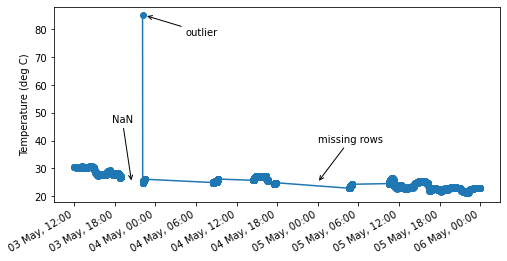
\includegraphics{outliers/temp-outlier.png}

While most measured points are between 20 and 30 °C, there is obviously
something very wrong with the one data point above 80 °C.

How could such a thing come about? This could be the result of
non-natural causes, such as measurement errors, wrong data collection,
or wrong data entry. On the other hand, this point could have natural
sources, such as a very hot spark flying next to the temperature sensor.

Identifying outliers is important, because they might greatly impact
measures like mean and standard deviation. When left untouched, outliers
might make us reach wrong conclusions about our data. See what happens
to the slope of this linear regression with and without the outliers.

\begin{figure}

{\centering 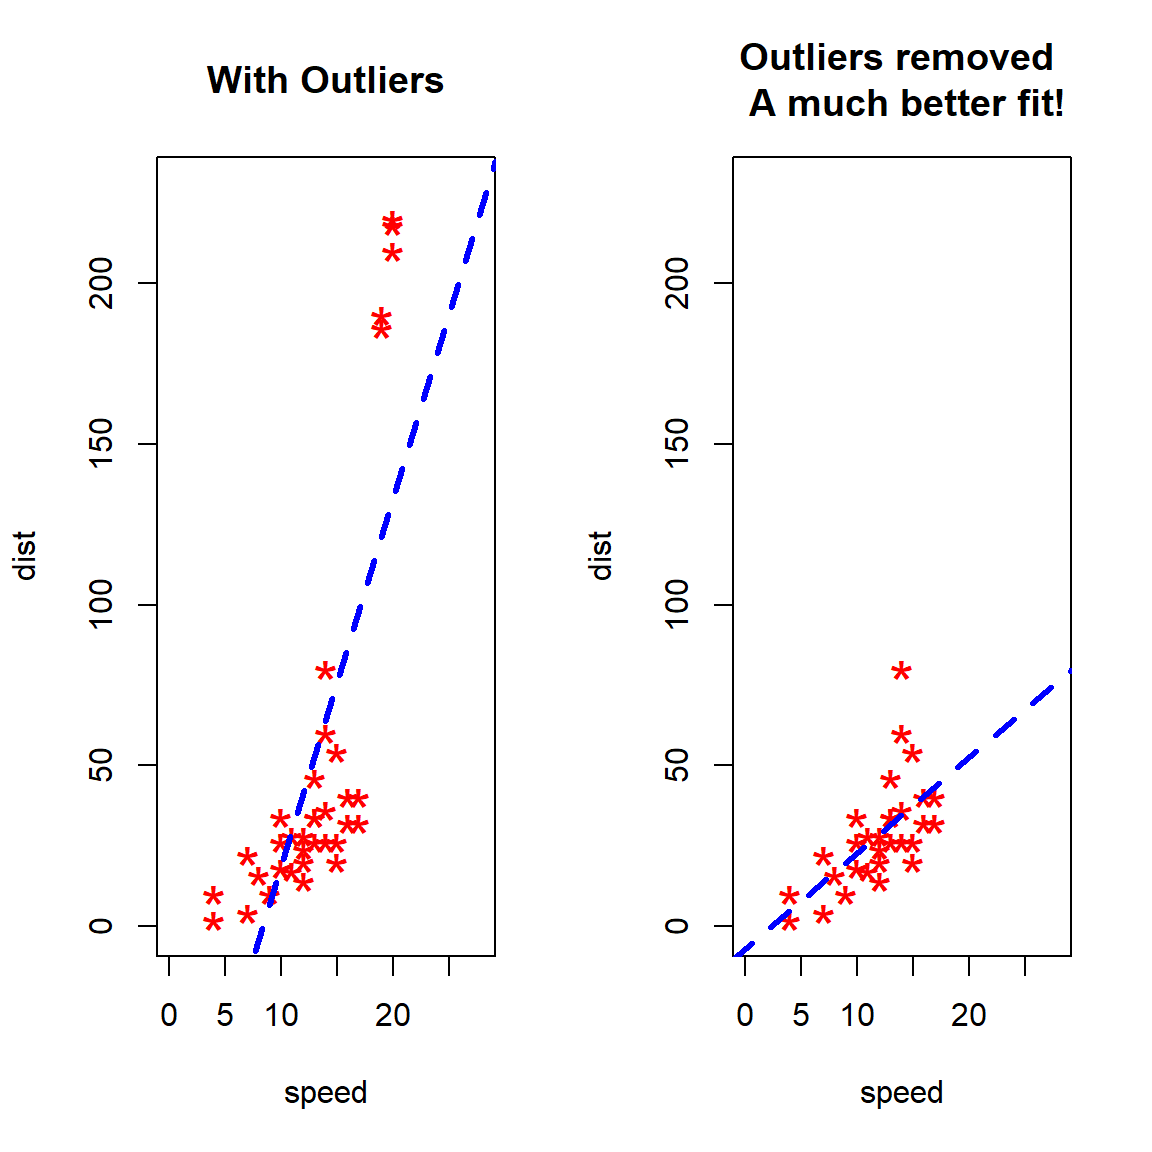
\includegraphics{outliers/regression-outlier.png}

}

\caption{Source: Zhang (2020)}

\end{figure}

\hypertarget{z-score}{%
\chapter{Z-score}\label{z-score}}

\[
z  = \frac{x-\mu}{\sigma},
\]

\marginnote{\begin{footnotesize}

where

\begin{itemize}
\tightlist
\item
  \(x=\) data point,\\
\item
  \(\mu=\) time series mean\\
\item
  \(\sigma=\) time series standard deviation.
\end{itemize}

\end{footnotesize}}

Let's write a function that identifies outliers according to the
Z-score.

\begin{Shaded}
\begin{Highlighting}[]
\KeywordTok{def}\NormalTok{ zscore(df, degree}\OperatorTok{=}\DecValTok{3}\NormalTok{):}
\NormalTok{    data }\OperatorTok{=}\NormalTok{ df.copy()}
\NormalTok{    data[}\StringTok{\textquotesingle{}zscore\textquotesingle{}}\NormalTok{] }\OperatorTok{=}\NormalTok{ (data }\OperatorTok{{-}}\NormalTok{ data.mean())}\OperatorTok{/}\NormalTok{data.std()}
\NormalTok{    outliers }\OperatorTok{=}\NormalTok{ data[(data[}\StringTok{\textquotesingle{}zscore\textquotesingle{}}\NormalTok{] }\OperatorTok{\textless{}=} \OperatorTok{{-}}\NormalTok{degree) }\OperatorTok{|}\NormalTok{ (data[}\StringTok{\textquotesingle{}zscore\textquotesingle{}}\NormalTok{] }\OperatorTok{\textgreater{}=}\NormalTok{ degree)]}
    \ControlFlowTok{return}\NormalTok{ outliers[}\StringTok{\textquotesingle{}value\textquotesingle{}}\NormalTok{], data}
\end{Highlighting}
\end{Shaded}

Now we can simply use this function:

\begin{Shaded}
\begin{Highlighting}[]
\NormalTok{threshold }\OperatorTok{=} \FloatTok{2.5}
\NormalTok{outliers, transformed }\OperatorTok{=}\NormalTok{ zscore(tx, threshold)}
\end{Highlighting}
\end{Shaded}

Source: Atwan (2022)

\hypertarget{iqr-inter-quartile-range}{%
\chapter{IQR (Inter Quartile Range)}\label{iqr-inter-quartile-range}}

The IQR (Inter Quartile Range) is the distance between the 25th
percentile (Q1) and the 75th percentile (Q3). In a box plot, the
whiskers usually extend \(1.5\times\)IQR beyond Q1 and Q3, see below.

\begin{figure}

{\centering 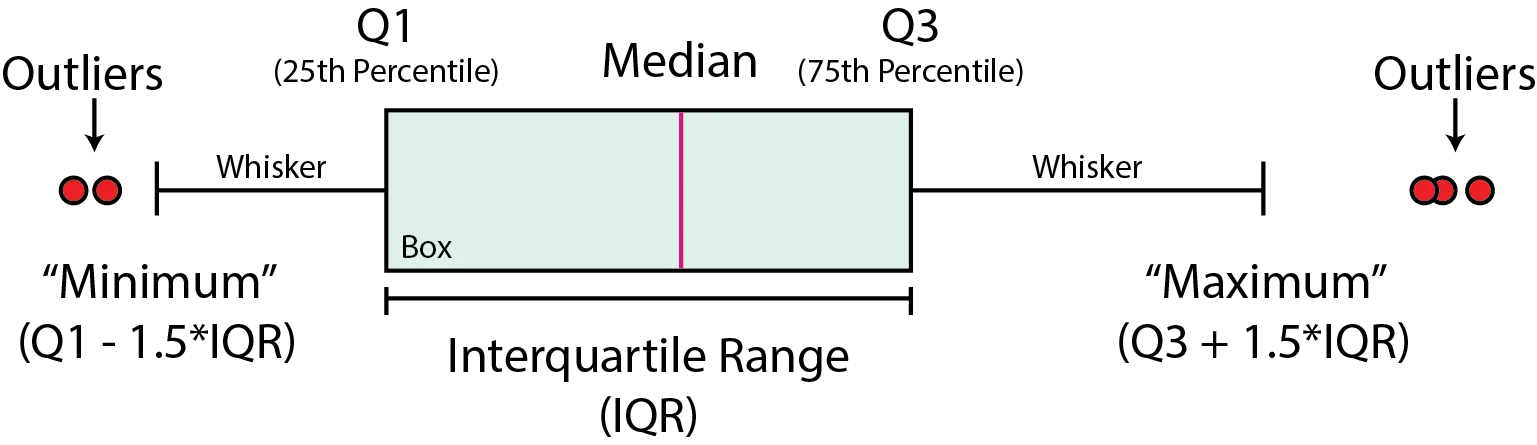
\includegraphics{outliers/iqr1.png}

}

\caption{Source: McDonald (2022)}

\end{figure}

A common outlier detection method is to consider whatever points outside
the whisker range as outliers.

\part{best practices}

\hypertarget{motivation-3}{%
\chapter{motivation}\label{motivation-3}}

\hypertarget{date-formatting}{%
\chapter{date formatting}\label{date-formatting}}

Here you will find several examples of how to format dates in your
plots. Not many explanations are provided.

How to use this page? Find first an example of a plot you like, only
then go to the code and see how it's done.

\begin{Shaded}
\begin{Highlighting}[]
\ImportTok{import}\NormalTok{ pandas }\ImportTok{as}\NormalTok{ pd}
\ImportTok{import}\NormalTok{ matplotlib.pyplot }\ImportTok{as}\NormalTok{ plt}
\ImportTok{import}\NormalTok{ numpy }\ImportTok{as}\NormalTok{ np}
\ImportTok{import}\NormalTok{ datetime}
\ImportTok{from}\NormalTok{ datetime }\ImportTok{import}\NormalTok{ timedelta}
\ImportTok{import}\NormalTok{ seaborn }\ImportTok{as}\NormalTok{ sns}
\NormalTok{sns.}\BuiltInTok{set}\NormalTok{(style}\OperatorTok{=}\StringTok{"ticks"}\NormalTok{, font\_scale}\OperatorTok{=}\FloatTok{1.5}\NormalTok{)}
\ImportTok{import}\NormalTok{ matplotlib.gridspec }\ImportTok{as}\NormalTok{ gridspec}
\ImportTok{from}\NormalTok{ matplotlib.dates }\ImportTok{import}\NormalTok{ DateFormatter}
\ImportTok{import}\NormalTok{ matplotlib.dates }\ImportTok{as}\NormalTok{ mdates}
\ImportTok{import}\NormalTok{ matplotlib.ticker }\ImportTok{as}\NormalTok{ ticker}
\end{Highlighting}
\end{Shaded}

\begin{Shaded}
\begin{Highlighting}[]
\ImportTok{import}\NormalTok{ pandas }\ImportTok{as}\NormalTok{ pd}

\NormalTok{start\_date }\OperatorTok{=} \StringTok{\textquotesingle{}2018{-}01{-}01\textquotesingle{}}
\NormalTok{end\_date }\OperatorTok{=} \StringTok{\textquotesingle{}2018{-}04{-}30\textquotesingle{}}

\CommentTok{\# create date range with 1{-}hour intervals}
\NormalTok{dates }\OperatorTok{=}\NormalTok{ pd.date\_range(start\_date, end\_date, freq}\OperatorTok{=}\StringTok{\textquotesingle{}1H\textquotesingle{}}\NormalTok{)}
\CommentTok{\# create a random variable to plot}
\NormalTok{var }\OperatorTok{=}\NormalTok{ np.random.rand(}\BuiltInTok{len}\NormalTok{(dates)) }\OperatorTok{{-}} \FloatTok{0.51}
\NormalTok{var }\OperatorTok{=}\NormalTok{ var.cumsum()}
\NormalTok{var }\OperatorTok{=}\NormalTok{ var }\OperatorTok{{-}}\NormalTok{ var.}\BuiltInTok{min}\NormalTok{()}
\CommentTok{\# create dataframe, make "date" the index}
\NormalTok{df }\OperatorTok{=}\NormalTok{ pd.DataFrame(\{}\StringTok{\textquotesingle{}date\textquotesingle{}}\NormalTok{: dates, }\StringTok{\textquotesingle{}variable\textquotesingle{}}\NormalTok{: var\})}
\NormalTok{df.set\_index(df[}\StringTok{\textquotesingle{}date\textquotesingle{}}\NormalTok{], inplace}\OperatorTok{=}\VariableTok{True}\NormalTok{)}
\NormalTok{df}
\end{Highlighting}
\end{Shaded}

\begin{longtable}[]{@{}lll@{}}
\toprule\noalign{}
& date & variable \\
date & & \\
\midrule\noalign{}
\endhead
\bottomrule\noalign{}
\endlastfoot
2018-01-01 00:00:00 & 2018-01-01 00:00:00 & 28.317035 \\
2018-01-01 01:00:00 & 2018-01-01 01:00:00 & 28.120523 \\
2018-01-01 02:00:00 & 2018-01-01 02:00:00 & 28.596894 \\
2018-01-01 03:00:00 & 2018-01-01 03:00:00 & 28.931941 \\
2018-01-01 04:00:00 & 2018-01-01 04:00:00 & 28.561778 \\
... & ... & ... \\
2018-04-29 20:00:00 & 2018-04-29 20:00:00 & 1.914343 \\
2018-04-29 21:00:00 & 2018-04-29 21:00:00 & 1.648757 \\
2018-04-29 22:00:00 & 2018-04-29 22:00:00 & 1.992956 \\
2018-04-29 23:00:00 & 2018-04-29 23:00:00 & 1.500860 \\
2018-04-30 00:00:00 & 2018-04-30 00:00:00 & 1.650439 \\
\end{longtable}

define a useful function to plot the graphs below

\begin{Shaded}
\begin{Highlighting}[]
\KeywordTok{def}\NormalTok{ explanation(ax, text, letter):}
\NormalTok{    ax.text(}\FloatTok{0.99}\NormalTok{, }\FloatTok{0.97}\NormalTok{, text,}
\NormalTok{            transform}\OperatorTok{=}\NormalTok{ax.transAxes,}
\NormalTok{            horizontalalignment}\OperatorTok{=}\StringTok{\textquotesingle{}right\textquotesingle{}}\NormalTok{, verticalalignment}\OperatorTok{=}\StringTok{\textquotesingle{}top\textquotesingle{}}\NormalTok{,}
\NormalTok{            fontweight}\OperatorTok{=}\StringTok{"bold"}\NormalTok{)}
\NormalTok{    ax.text(}\FloatTok{0.01}\NormalTok{, }\FloatTok{0.01}\NormalTok{, letter,}
\NormalTok{            transform}\OperatorTok{=}\NormalTok{ax.transAxes,}
\NormalTok{            horizontalalignment}\OperatorTok{=}\StringTok{\textquotesingle{}left\textquotesingle{}}\NormalTok{, verticalalignment}\OperatorTok{=}\StringTok{\textquotesingle{}bottom\textquotesingle{}}\NormalTok{,}
\NormalTok{            fontweight}\OperatorTok{=}\StringTok{"bold"}\NormalTok{)}
\NormalTok{    ax.}\BuiltInTok{set}\NormalTok{(ylabel}\OperatorTok{=}\StringTok{"variable (units)"}\NormalTok{)}
\NormalTok{    ax.spines[}\StringTok{\textquotesingle{}top\textquotesingle{}}\NormalTok{].set\_visible(}\VariableTok{False}\NormalTok{)}
\NormalTok{    ax.spines[}\StringTok{\textquotesingle{}right\textquotesingle{}}\NormalTok{].set\_visible(}\VariableTok{False}\NormalTok{)}
\end{Highlighting}
\end{Shaded}

\begin{Shaded}
\begin{Highlighting}[]
\NormalTok{fig, ax }\OperatorTok{=}\NormalTok{ plt.subplots(}\DecValTok{1}\NormalTok{, }\DecValTok{1}\NormalTok{, figsize}\OperatorTok{=}\NormalTok{(}\DecValTok{8}\NormalTok{, }\DecValTok{6}\NormalTok{))}
\NormalTok{ax.plot(df[}\StringTok{\textquotesingle{}variable\textquotesingle{}}\NormalTok{])}
\NormalTok{plt.gcf().autofmt\_xdate()  }\CommentTok{\# makes slated dates}
\NormalTok{explanation(ax, }\StringTok{"slanted dates"}\NormalTok{, }\StringTok{""}\NormalTok{)}
\NormalTok{fig.savefig(}\StringTok{"dates1.png"}\NormalTok{)}
\end{Highlighting}
\end{Shaded}

\begin{figure}[H]

{\centering \includegraphics{best-practices/date-formatting_files/figure-pdf/cell-5-output-1.png}

}

\end{figure}

\begin{Shaded}
\begin{Highlighting}[]
\NormalTok{fig, ax }\OperatorTok{=}\NormalTok{ plt.subplots(}\DecValTok{4}\NormalTok{, }\DecValTok{1}\NormalTok{, figsize}\OperatorTok{=}\NormalTok{(}\DecValTok{10}\NormalTok{, }\DecValTok{16}\NormalTok{),}
\NormalTok{                       gridspec\_kw}\OperatorTok{=}\NormalTok{\{}\StringTok{\textquotesingle{}hspace\textquotesingle{}}\NormalTok{: }\FloatTok{0.3}\NormalTok{\})}

\CommentTok{\#\#\# plot a }\AlertTok{\#\#\#}
\NormalTok{ax[}\DecValTok{0}\NormalTok{].plot(df[}\StringTok{\textquotesingle{}variable\textquotesingle{}}\NormalTok{])}
\NormalTok{date\_form }\OperatorTok{=}\NormalTok{ DateFormatter(}\StringTok{"\%b"}\NormalTok{)}
\NormalTok{ax[}\DecValTok{0}\NormalTok{].xaxis.set\_major\_locator(mdates.MonthLocator(interval}\OperatorTok{=}\DecValTok{2}\NormalTok{))}
\NormalTok{ax[}\DecValTok{0}\NormalTok{].xaxis.set\_major\_formatter(date\_form)}

\CommentTok{\#\#\# plot b }\AlertTok{\#\#\#}
\NormalTok{ax[}\DecValTok{1}\NormalTok{].plot(df[}\StringTok{\textquotesingle{}variable\textquotesingle{}}\NormalTok{])}
\NormalTok{date\_form }\OperatorTok{=}\NormalTok{ DateFormatter(}\StringTok{"\%B"}\NormalTok{)}
\NormalTok{ax[}\DecValTok{1}\NormalTok{].xaxis.set\_major\_locator(mdates.MonthLocator(interval}\OperatorTok{=}\DecValTok{1}\NormalTok{))}
\NormalTok{ax[}\DecValTok{1}\NormalTok{].xaxis.set\_major\_formatter(date\_form)}

\CommentTok{\#\#\# plot c }\AlertTok{\#\#\#}
\NormalTok{ax[}\DecValTok{2}\NormalTok{].plot(df[}\StringTok{\textquotesingle{}variable\textquotesingle{}}\NormalTok{])}
\NormalTok{ax[}\DecValTok{2}\NormalTok{].xaxis.set\_major\_locator(mdates.MonthLocator())}
\CommentTok{\# 16 is a slight approximation for the center, since months differ in number of days.}
\NormalTok{ax[}\DecValTok{2}\NormalTok{].xaxis.set\_minor\_locator(mdates.MonthLocator(bymonthday}\OperatorTok{=}\DecValTok{16}\NormalTok{))}
\NormalTok{ax[}\DecValTok{2}\NormalTok{].xaxis.set\_major\_formatter(ticker.NullFormatter())}
\NormalTok{ax[}\DecValTok{2}\NormalTok{].xaxis.set\_minor\_formatter(DateFormatter(}\StringTok{\textquotesingle{}\%B\textquotesingle{}}\NormalTok{))}
\ControlFlowTok{for}\NormalTok{ tick }\KeywordTok{in}\NormalTok{ ax[}\DecValTok{2}\NormalTok{].xaxis.get\_minor\_ticks():}
\NormalTok{    tick.tick1line.set\_markersize(}\DecValTok{0}\NormalTok{)}
\NormalTok{    tick.tick2line.set\_markersize(}\DecValTok{0}\NormalTok{)}
\NormalTok{    tick.label1.set\_horizontalalignment(}\StringTok{\textquotesingle{}center\textquotesingle{}}\NormalTok{)}

\CommentTok{\#\#\# plot d }\AlertTok{\#\#\#}
\NormalTok{ax[}\DecValTok{3}\NormalTok{].plot(df[}\StringTok{\textquotesingle{}variable\textquotesingle{}}\NormalTok{])}
\NormalTok{date\_form }\OperatorTok{=}\NormalTok{ DateFormatter(}\StringTok{"}\SpecialCharTok{\%d}\StringTok{ \%b"}\NormalTok{)}
\NormalTok{ax[}\DecValTok{3}\NormalTok{].xaxis.set\_major\_locator(mdates.DayLocator(interval}\OperatorTok{=}\DecValTok{15}\NormalTok{))}
\NormalTok{ax[}\DecValTok{3}\NormalTok{].xaxis.set\_major\_formatter(date\_form)}

\NormalTok{explanation(ax[}\DecValTok{0}\NormalTok{], }\StringTok{"month abbreviations, every 2 months"}\NormalTok{, }\StringTok{"a"}\NormalTok{)}
\NormalTok{explanation(ax[}\DecValTok{1}\NormalTok{], }\StringTok{"full month names"}\NormalTok{, }\StringTok{"b"}\NormalTok{)}
\NormalTok{explanation(ax[}\DecValTok{2}\NormalTok{], }\StringTok{"full month names centered between the 1st of the month"}\NormalTok{, }\StringTok{"c"}\NormalTok{)}
\NormalTok{explanation(ax[}\DecValTok{3}\NormalTok{], }\StringTok{"day + month abbr. {-}{-}{-} every 15 days"}\NormalTok{, }\StringTok{"d"}\NormalTok{)}

\NormalTok{fig.savefig(}\StringTok{"dates2.png"}\NormalTok{)}
\end{Highlighting}
\end{Shaded}

\begin{figure}[H]

{\centering \includegraphics{best-practices/date-formatting_files/figure-pdf/cell-6-output-1.png}

}

\end{figure}

\begin{Shaded}
\begin{Highlighting}[]
\NormalTok{fig, ax }\OperatorTok{=}\NormalTok{ plt.subplots(}\DecValTok{4}\NormalTok{, }\DecValTok{1}\NormalTok{, figsize}\OperatorTok{=}\NormalTok{(}\DecValTok{10}\NormalTok{, }\DecValTok{16}\NormalTok{),}
\NormalTok{                       gridspec\_kw}\OperatorTok{=}\NormalTok{\{}\StringTok{\textquotesingle{}hspace\textquotesingle{}}\NormalTok{: }\FloatTok{0.3}\NormalTok{\})}

\CommentTok{\#\#\# plot e }\AlertTok{\#\#\#}
\NormalTok{ax[}\DecValTok{0}\NormalTok{].plot(df[}\StringTok{\textquotesingle{}variable\textquotesingle{}}\NormalTok{])}
\NormalTok{date\_form }\OperatorTok{=}\NormalTok{ DateFormatter(}\StringTok{"}\SpecialCharTok{\%d}\StringTok{/\%m"}\NormalTok{)}
\NormalTok{ax[}\DecValTok{0}\NormalTok{].xaxis.set\_major\_locator(mdates.DayLocator(bymonthday}\OperatorTok{=}\NormalTok{[}\DecValTok{5}\NormalTok{, }\DecValTok{20}\NormalTok{]))}
\NormalTok{ax[}\DecValTok{0}\NormalTok{].xaxis.set\_major\_formatter(date\_form)}

\CommentTok{\#\#\# plot f }\AlertTok{\#\#\#}
\NormalTok{ax[}\DecValTok{1}\NormalTok{].plot(df[}\StringTok{\textquotesingle{}variable\textquotesingle{}}\NormalTok{])}
\NormalTok{locator }\OperatorTok{=}\NormalTok{ mdates.AutoDateLocator(minticks}\OperatorTok{=}\DecValTok{11}\NormalTok{, maxticks}\OperatorTok{=}\DecValTok{17}\NormalTok{)}
\NormalTok{formatter }\OperatorTok{=}\NormalTok{ mdates.ConciseDateFormatter(locator)}
\NormalTok{ax[}\DecValTok{1}\NormalTok{].xaxis.set\_major\_locator(locator)}
\NormalTok{ax[}\DecValTok{1}\NormalTok{].xaxis.set\_major\_formatter(formatter)}

\CommentTok{\#\#\# plot g }\AlertTok{\#\#\#}
\NormalTok{ax[}\DecValTok{2}\NormalTok{].plot(df.loc[}\StringTok{\textquotesingle{}2018{-}01{-}01\textquotesingle{}}\NormalTok{:}\StringTok{\textquotesingle{}2018{-}03{-}01\textquotesingle{}}\NormalTok{, }\StringTok{\textquotesingle{}variable\textquotesingle{}}\NormalTok{])}
\NormalTok{locator }\OperatorTok{=}\NormalTok{ mdates.AutoDateLocator(minticks}\OperatorTok{=}\DecValTok{6}\NormalTok{, maxticks}\OperatorTok{=}\DecValTok{14}\NormalTok{)}
\NormalTok{formatter }\OperatorTok{=}\NormalTok{ mdates.ConciseDateFormatter(locator)}
\NormalTok{ax[}\DecValTok{2}\NormalTok{].xaxis.set\_major\_locator(locator)}
\NormalTok{ax[}\DecValTok{2}\NormalTok{].xaxis.set\_major\_formatter(formatter)}

\CommentTok{\#\#\# plot h }\AlertTok{\#\#\#}
\NormalTok{ax[}\DecValTok{3}\NormalTok{].plot(df.loc[}\StringTok{\textquotesingle{}2018{-}01{-}01\textquotesingle{}}\NormalTok{:}\StringTok{\textquotesingle{}2018{-}01{-}02\textquotesingle{}}\NormalTok{, }\StringTok{\textquotesingle{}variable\textquotesingle{}}\NormalTok{])}
\NormalTok{locator }\OperatorTok{=}\NormalTok{ mdates.AutoDateLocator(minticks}\OperatorTok{=}\DecValTok{6}\NormalTok{, maxticks}\OperatorTok{=}\DecValTok{10}\NormalTok{)}
\NormalTok{formatter }\OperatorTok{=}\NormalTok{ mdates.ConciseDateFormatter(locator)}
\NormalTok{ax[}\DecValTok{3}\NormalTok{].xaxis.set\_major\_locator(locator)}
\NormalTok{ax[}\DecValTok{3}\NormalTok{].xaxis.set\_major\_formatter(formatter)}

\NormalTok{explanation(ax[}\DecValTok{0}\NormalTok{], }\StringTok{"exactly on days 05 and 20 of each month"}\NormalTok{, }\StringTok{"e"}\NormalTok{)}
\NormalTok{explanation(ax[}\DecValTok{1}\NormalTok{], }\StringTok{"ConciseDateFormatter"}\NormalTok{, }\StringTok{"f"}\NormalTok{)}
\NormalTok{explanation(ax[}\DecValTok{2}\NormalTok{], }\StringTok{"ConciseDateFormatter"}\NormalTok{, }\StringTok{"g"}\NormalTok{)}
\NormalTok{explanation(ax[}\DecValTok{3}\NormalTok{], }\StringTok{"ConciseDateFormatter"}\NormalTok{, }\StringTok{"h"}\NormalTok{)}

\NormalTok{fig.savefig(}\StringTok{"dates3.png"}\NormalTok{)}
\end{Highlighting}
\end{Shaded}

\begin{figure}[H]

{\centering \includegraphics{best-practices/date-formatting_files/figure-pdf/cell-7-output-1.png}

}

\end{figure}

\begin{Shaded}
\begin{Highlighting}[]
\NormalTok{fig, ax }\OperatorTok{=}\NormalTok{ plt.subplots(}\DecValTok{1}\NormalTok{, }\DecValTok{1}\NormalTok{, figsize}\OperatorTok{=}\NormalTok{(}\DecValTok{10}\NormalTok{, }\DecValTok{4}\NormalTok{),}
\NormalTok{                       gridspec\_kw}\OperatorTok{=}\NormalTok{\{}\StringTok{\textquotesingle{}hspace\textquotesingle{}}\NormalTok{: }\FloatTok{0.3}\NormalTok{\})}

\CommentTok{\# import constants for the days of the week}
\ImportTok{from}\NormalTok{ matplotlib.dates }\ImportTok{import}\NormalTok{ MO, TU, WE, TH, FR, SA, SU}
\NormalTok{ax.plot(df[}\StringTok{\textquotesingle{}variable\textquotesingle{}}\NormalTok{])}
\CommentTok{\# tick on sundays every third week}
\NormalTok{loc }\OperatorTok{=}\NormalTok{ mdates.WeekdayLocator(byweekday}\OperatorTok{=}\NormalTok{SU, interval}\OperatorTok{=}\DecValTok{3}\NormalTok{)}
\NormalTok{ax.xaxis.set\_major\_locator(loc)}
\NormalTok{date\_form }\OperatorTok{=}\NormalTok{ DateFormatter(}\StringTok{"\%a, \%b }\SpecialCharTok{\%d}\StringTok{"}\NormalTok{)}
\NormalTok{ax.xaxis.set\_major\_formatter(date\_form)}
\NormalTok{fig.autofmt\_xdate(bottom}\OperatorTok{=}\FloatTok{0.2}\NormalTok{, rotation}\OperatorTok{=}\DecValTok{30}\NormalTok{, ha}\OperatorTok{=}\StringTok{\textquotesingle{}right\textquotesingle{}}\NormalTok{)}
\NormalTok{explanation(ax, }\StringTok{"every 3 Sundays, rotate labels"}\NormalTok{, }\StringTok{""}\NormalTok{)}
\end{Highlighting}
\end{Shaded}

\begin{figure}[H]

{\centering \includegraphics{best-practices/date-formatting_files/figure-pdf/cell-8-output-1.png}

}

\end{figure}

\begin{longtable}[]{@{}ll@{}}
\toprule\noalign{}
Code & Explanation \\
\midrule\noalign{}
\endhead
\bottomrule\noalign{}
\endlastfoot
\%Y & 4-digit year (e.g., 2022) \\
\%y & 2-digit year (e.g., 22) \\
\%m & 2-digit month (e.g., 12) \\
\%B & Full month name (e.g., December) \\
\%b & Abbreviated month name (e.g., Dec) \\
\%d & 2-digit day of the month (e.g., 09) \\
\%A & Full weekday name (e.g., Tuesday) \\
\%a & Abbreviated weekday name (e.g., Tue) \\
\%H & 24-hour clock hour (e.g., 23) \\
\%I & 12-hour clock hour (e.g., 11) \\
\%M & 2-digit minute (e.g., 59) \\
\%S & 2-digit second (e.g., 59) \\
\%p & ``AM'' or ``PM'' \\
\%Z & Time zone name \\
\%z & Time zone offset from UTC (e.g., -0500) \\
\end{longtable}

\part{stationarity}

\hypertarget{motivation-4}{%
\chapter{motivation}\label{motivation-4}}

\hypertarget{stochastic-processes}{%
\chapter{stochastic processes}\label{stochastic-processes}}

\hypertarget{autocorrelation}{%
\chapter{autocorrelation}\label{autocorrelation}}

See the temperatures for Jerusalem in a 4-day interval:

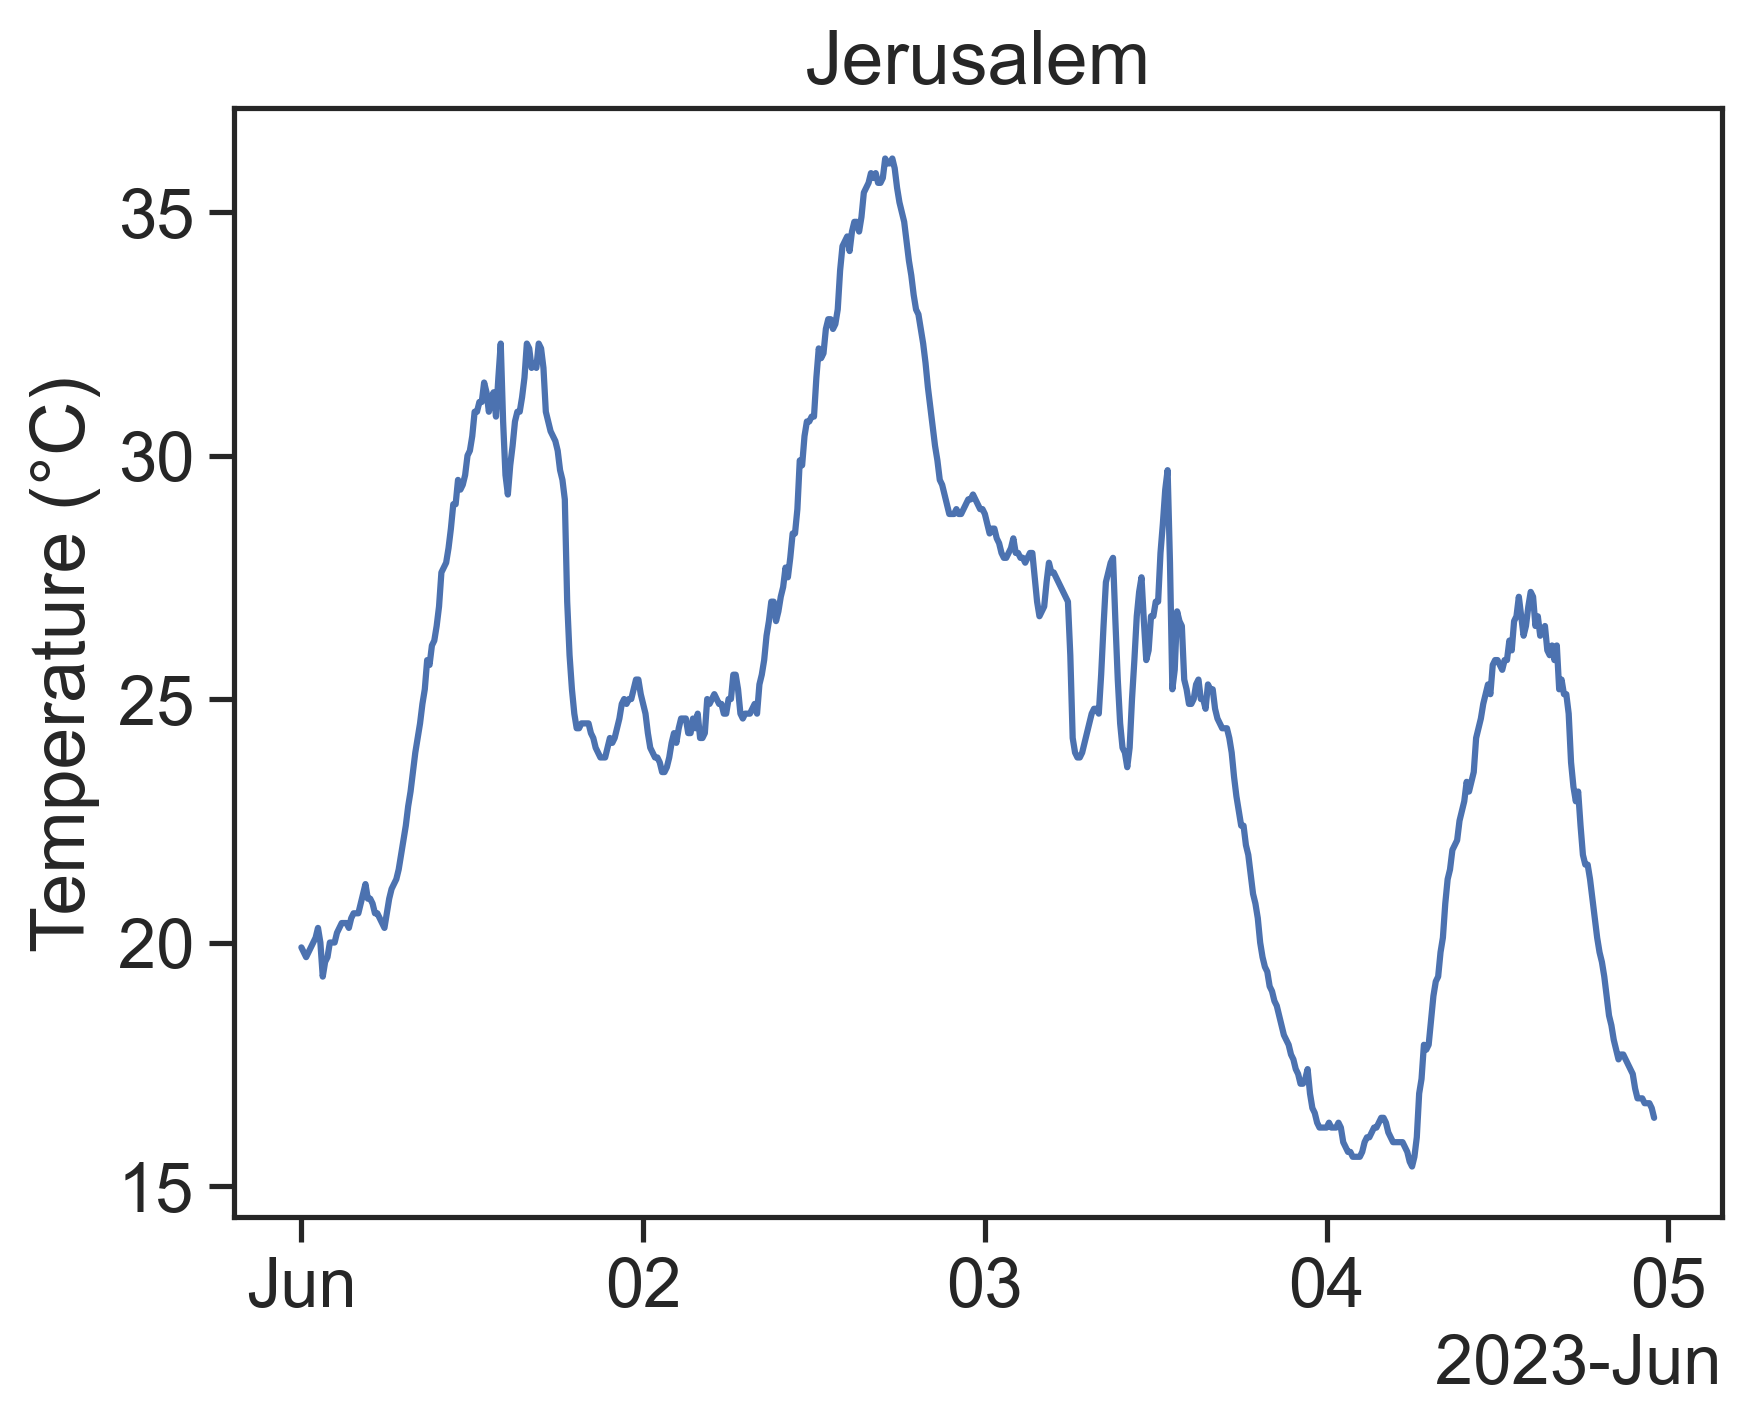
\includegraphics{stationarity/jer_temp1.png}

\hypertarget{question}{%
\section{question}\label{question}}

If I know the temperature right now, what does that tell me about the
temperature 10 minutes from now? How about 100 minutes? 1000 minutes?

To answer this, we need to talk about \textbf{autocorrelation}. Let's
start by introducing the necessary concepts.

\hypertarget{mean-and-standard-deviation}{%
\section{mean and standard
deviation}\label{mean-and-standard-deviation}}

Let's call our time series from above \(X\), and its length \(N\). Then:

\[
\begin{aligned}
\text{mean}& &\mu &= \frac{\displaystyle\sum_{i=1}^N X_i}{N} \\
\text{standard deviation}& &\sigma &= \sqrt{\frac{\displaystyle\sum_{i=1}^N (X_i-\mu)^2}{N}}
\end{aligned}
\]

The mean and standard deviation can be visualized thus:

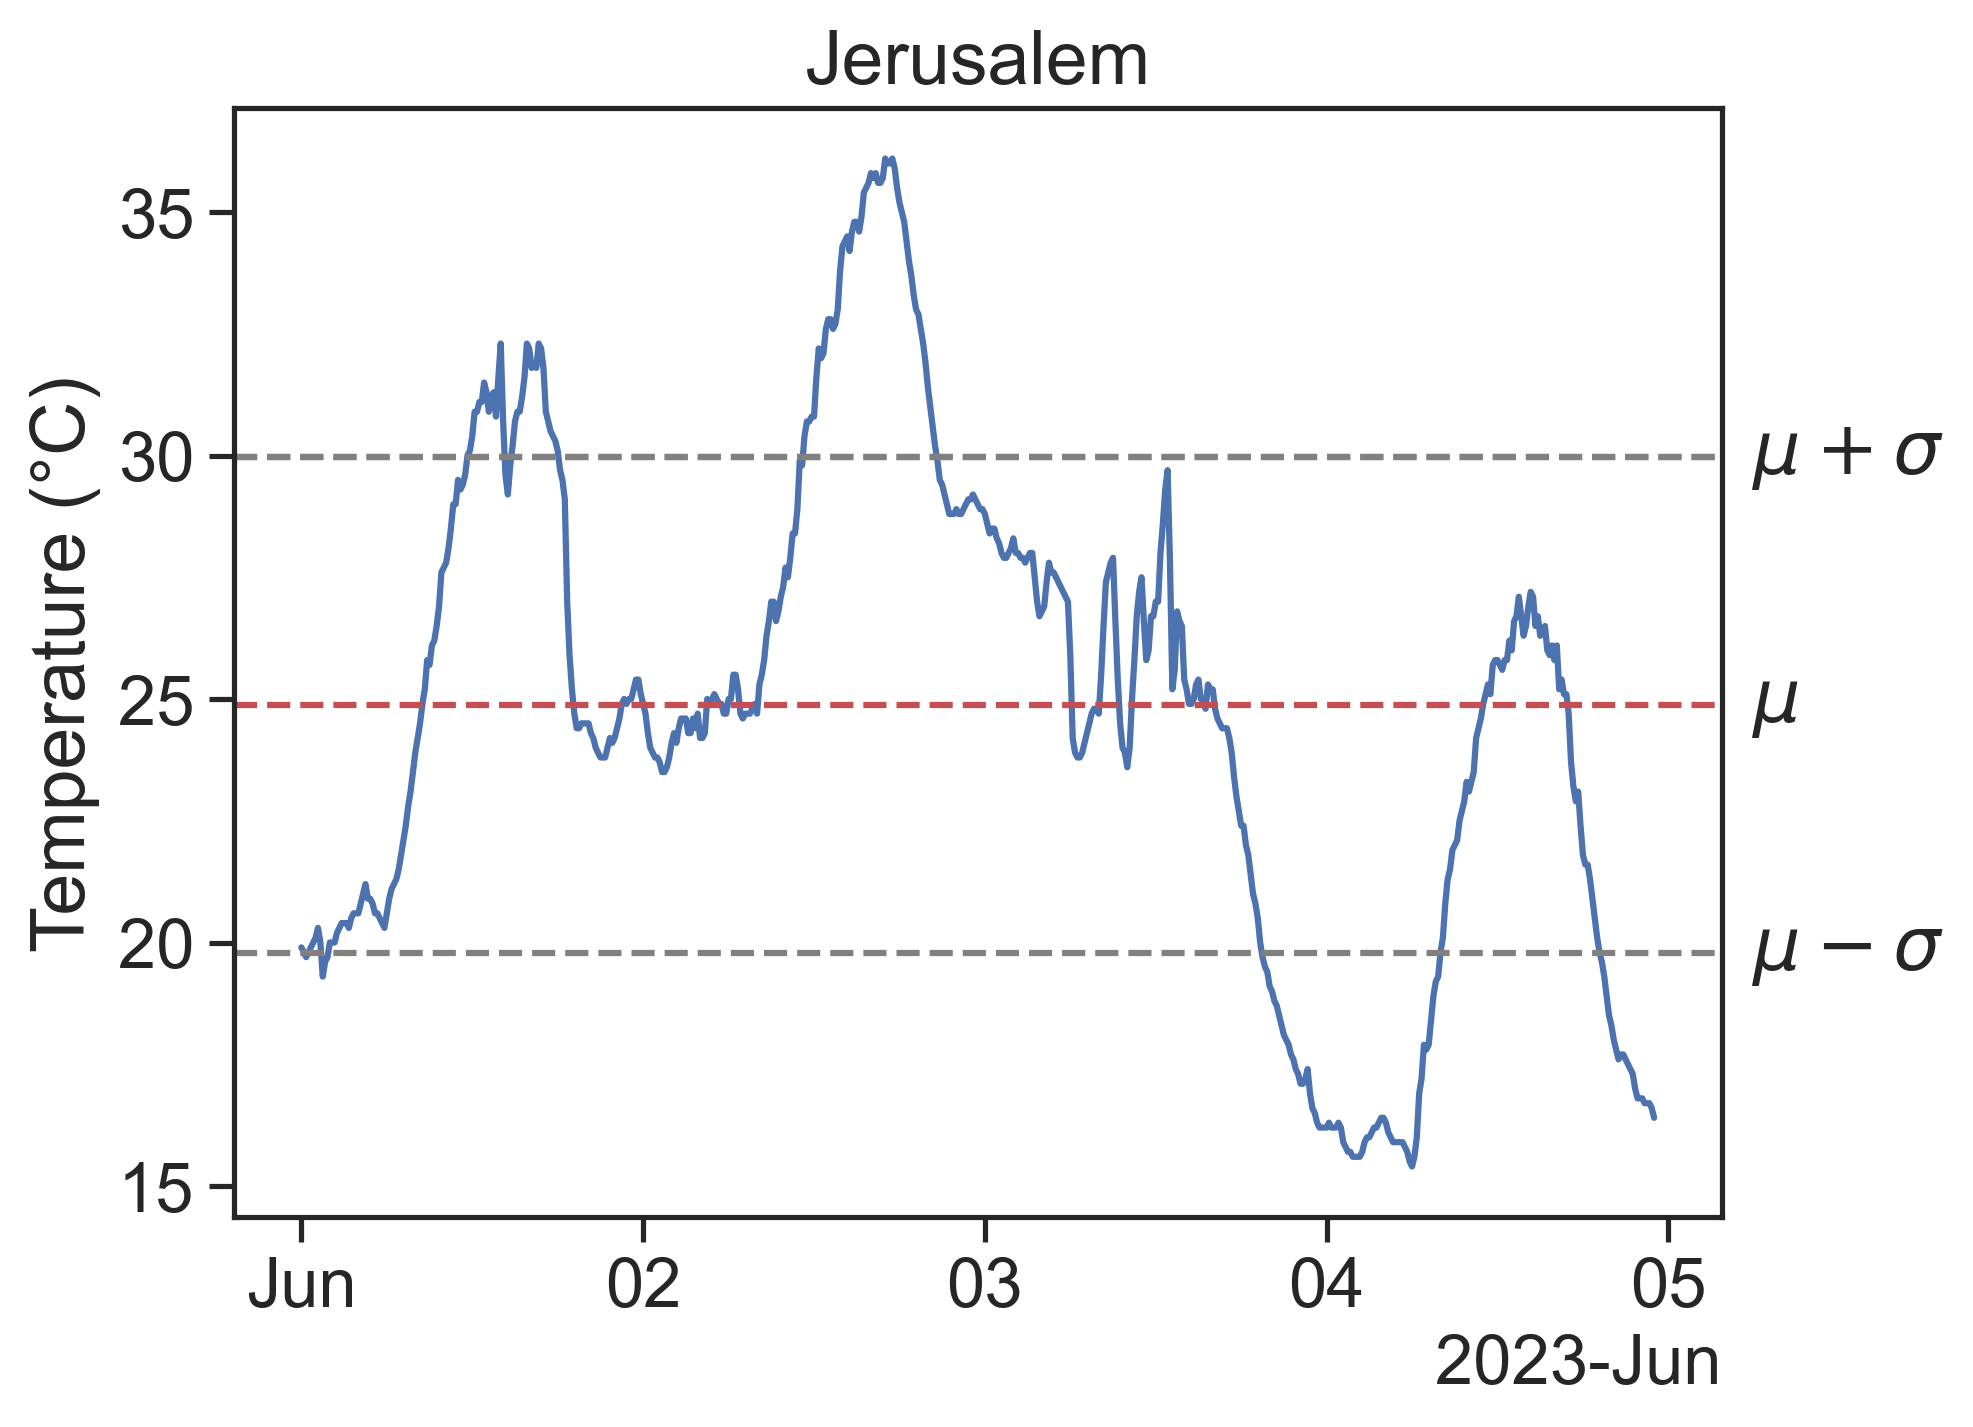
\includegraphics{stationarity/jer_temp2.png}

One last basic concept we need is the expected value: \[
E[X] = \sum_{i=1}^N X_i p_i
\]

For our time series, the probability \(p_i\) that a given point \(X_i\)
is in the dataset is simply \(1/N\), therefore the expectation becomes

\[
E[X] = \frac{\displaystyle\sum_{i=1}^N X_i}{N}
\]

\hypertarget{autocorrelation-1}{%
\section{autocorrelation}\label{autocorrelation-1}}

The autocorrelation of a time series \(X\) is the answer to the
following question:

\begin{quote}
if we shift \(X\) by \(\tau\) units, how similar will this be to the
original signal?
\end{quote}

In other words:

\begin{quote}
how correlated are \(X(t)\) and \(X(t+\tau)\)?
\end{quote}

Using the Pearson correlation coefficient

\marginnote{\begin{footnotesize}

Pearson correlation coefficient between \(X\) and \(Y\): \[
\rho_{X,Y} = \frac{E\left[ (X - \mu_X)(X_Y - \mu_Y) \right]}{\sigma_X\sigma_Y}
\]

\end{footnotesize}}

we get

\[
\rho_{XX}(\tau) = \frac{E\left[ (X_t - \mu)(X_{t+\tau} - \mu) \right]}{\sigma^2}
\]

A video is worth a billion words, so let's see the autocorrelation in
action:

\url{https://youtu.be/tpf-tuYHR5w}

A few comments:

\begin{itemize}
\tightlist
\item
  The autocorrelation for \(\tau=0\) (zero shift) is always 1.\\
  {[}Can you prove this? All the necessary equations are above!{]}
\end{itemize}

\part{time lags}

\hypertarget{motivation-5}{%
\chapter{motivation}\label{motivation-5}}

\hypertarget{cross-correlation}{%
\chapter{cross-correlation}\label{cross-correlation}}

\begin{Shaded}
\begin{Highlighting}[]
\ImportTok{import}\NormalTok{ numpy }\ImportTok{as}\NormalTok{ np}
\end{Highlighting}
\end{Shaded}

\begin{Shaded}
\begin{Highlighting}[]
\BuiltInTok{print}\NormalTok{(}\StringTok{\textquotesingle{}dfvdfv\textquotesingle{}}\NormalTok{)}
\end{Highlighting}
\end{Shaded}

\begin{verbatim}
dfvdfv
\end{verbatim}

\hypertarget{dynamic-time-warp}{%
\chapter{dynamic time warp}\label{dynamic-time-warp}}

\hypertarget{ldtw}{%
\chapter{LDTW}\label{ldtw}}

according to this paper

\part{frequency}

\hypertarget{motivation-6}{%
\chapter{motivation}\label{motivation-6}}

\hypertarget{fourier-transform}{%
\chapter{Fourier transform}\label{fourier-transform}}

\hypertarget{basic-wave-concepts}{%
\section{basic wave concepts}\label{basic-wave-concepts}}

The function

\begin{equation}\protect\hypertarget{eq-sin-Bf}{}{
f(t) = B\sin(2\pi f t)
}\label{eq-sin-Bf}\end{equation}

has two basic characteristics, its amplitude \(B\) and frequency \(f\).

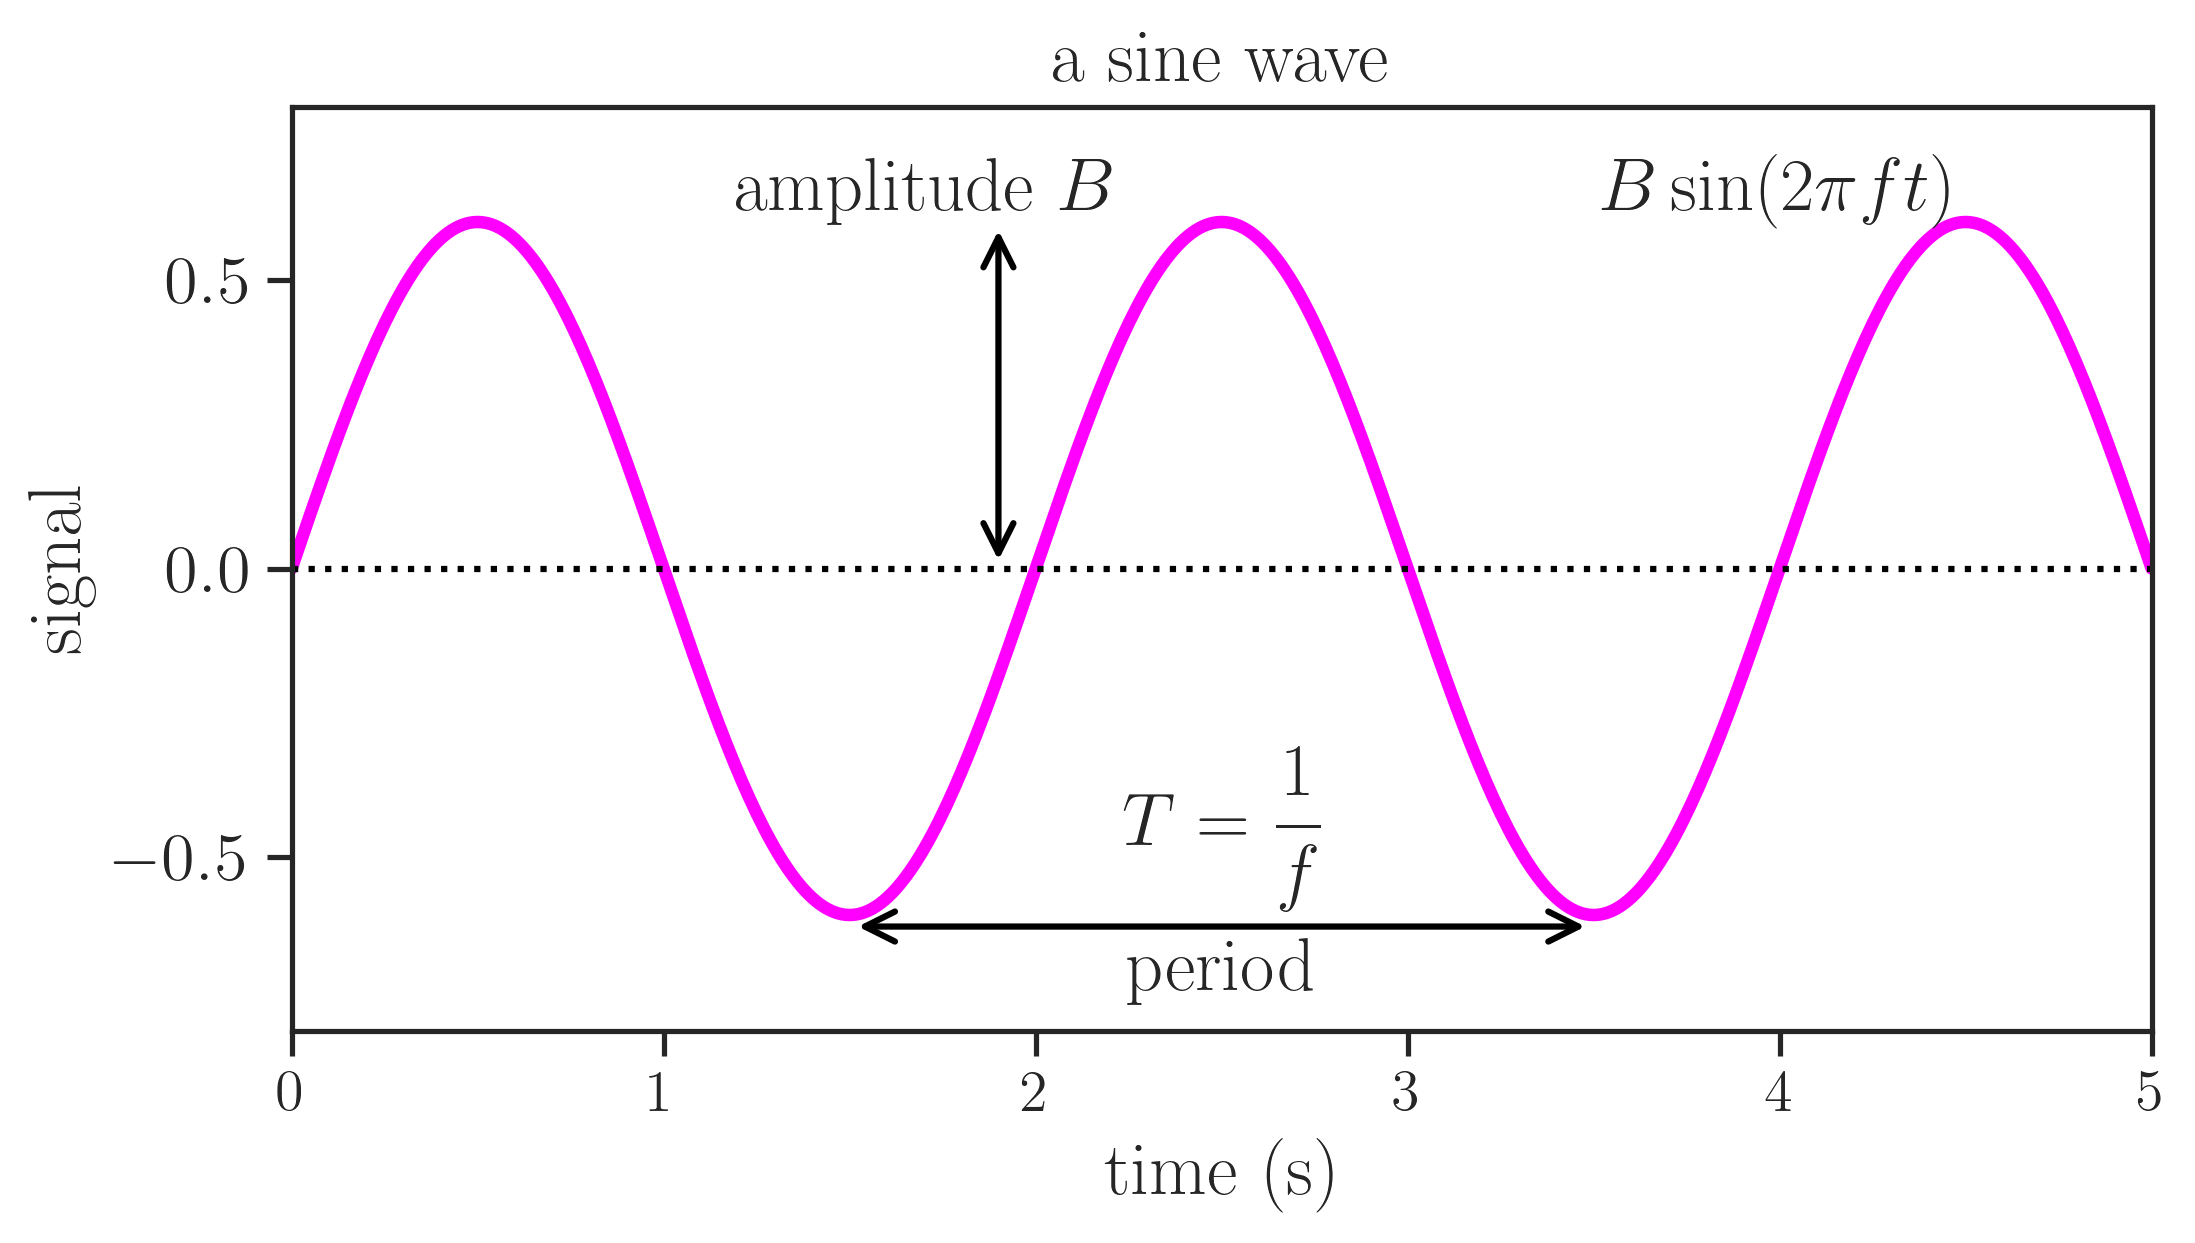
\includegraphics{frequency/sine1.png}

In the figure above, the amplitude \(B=0.6\) and we see that the
distance between two peaks is called period, \(T=2\) s. The frequency is
defined as the inverse of the period:

\begin{equation}\protect\hypertarget{eq-fT}{}{
f = \frac{1}{T}.
}\label{eq-fT}\end{equation}

When time is in seconds, then the frequency is measured in Hertz (Hz).
For the graph above, therefore, we see a wave whose frequency is
\(f = 1/(2 \text{ s}) = 0.5\) Hz.

In the figure below, we see what happens when we vary the values of the
frequency and amplitude.

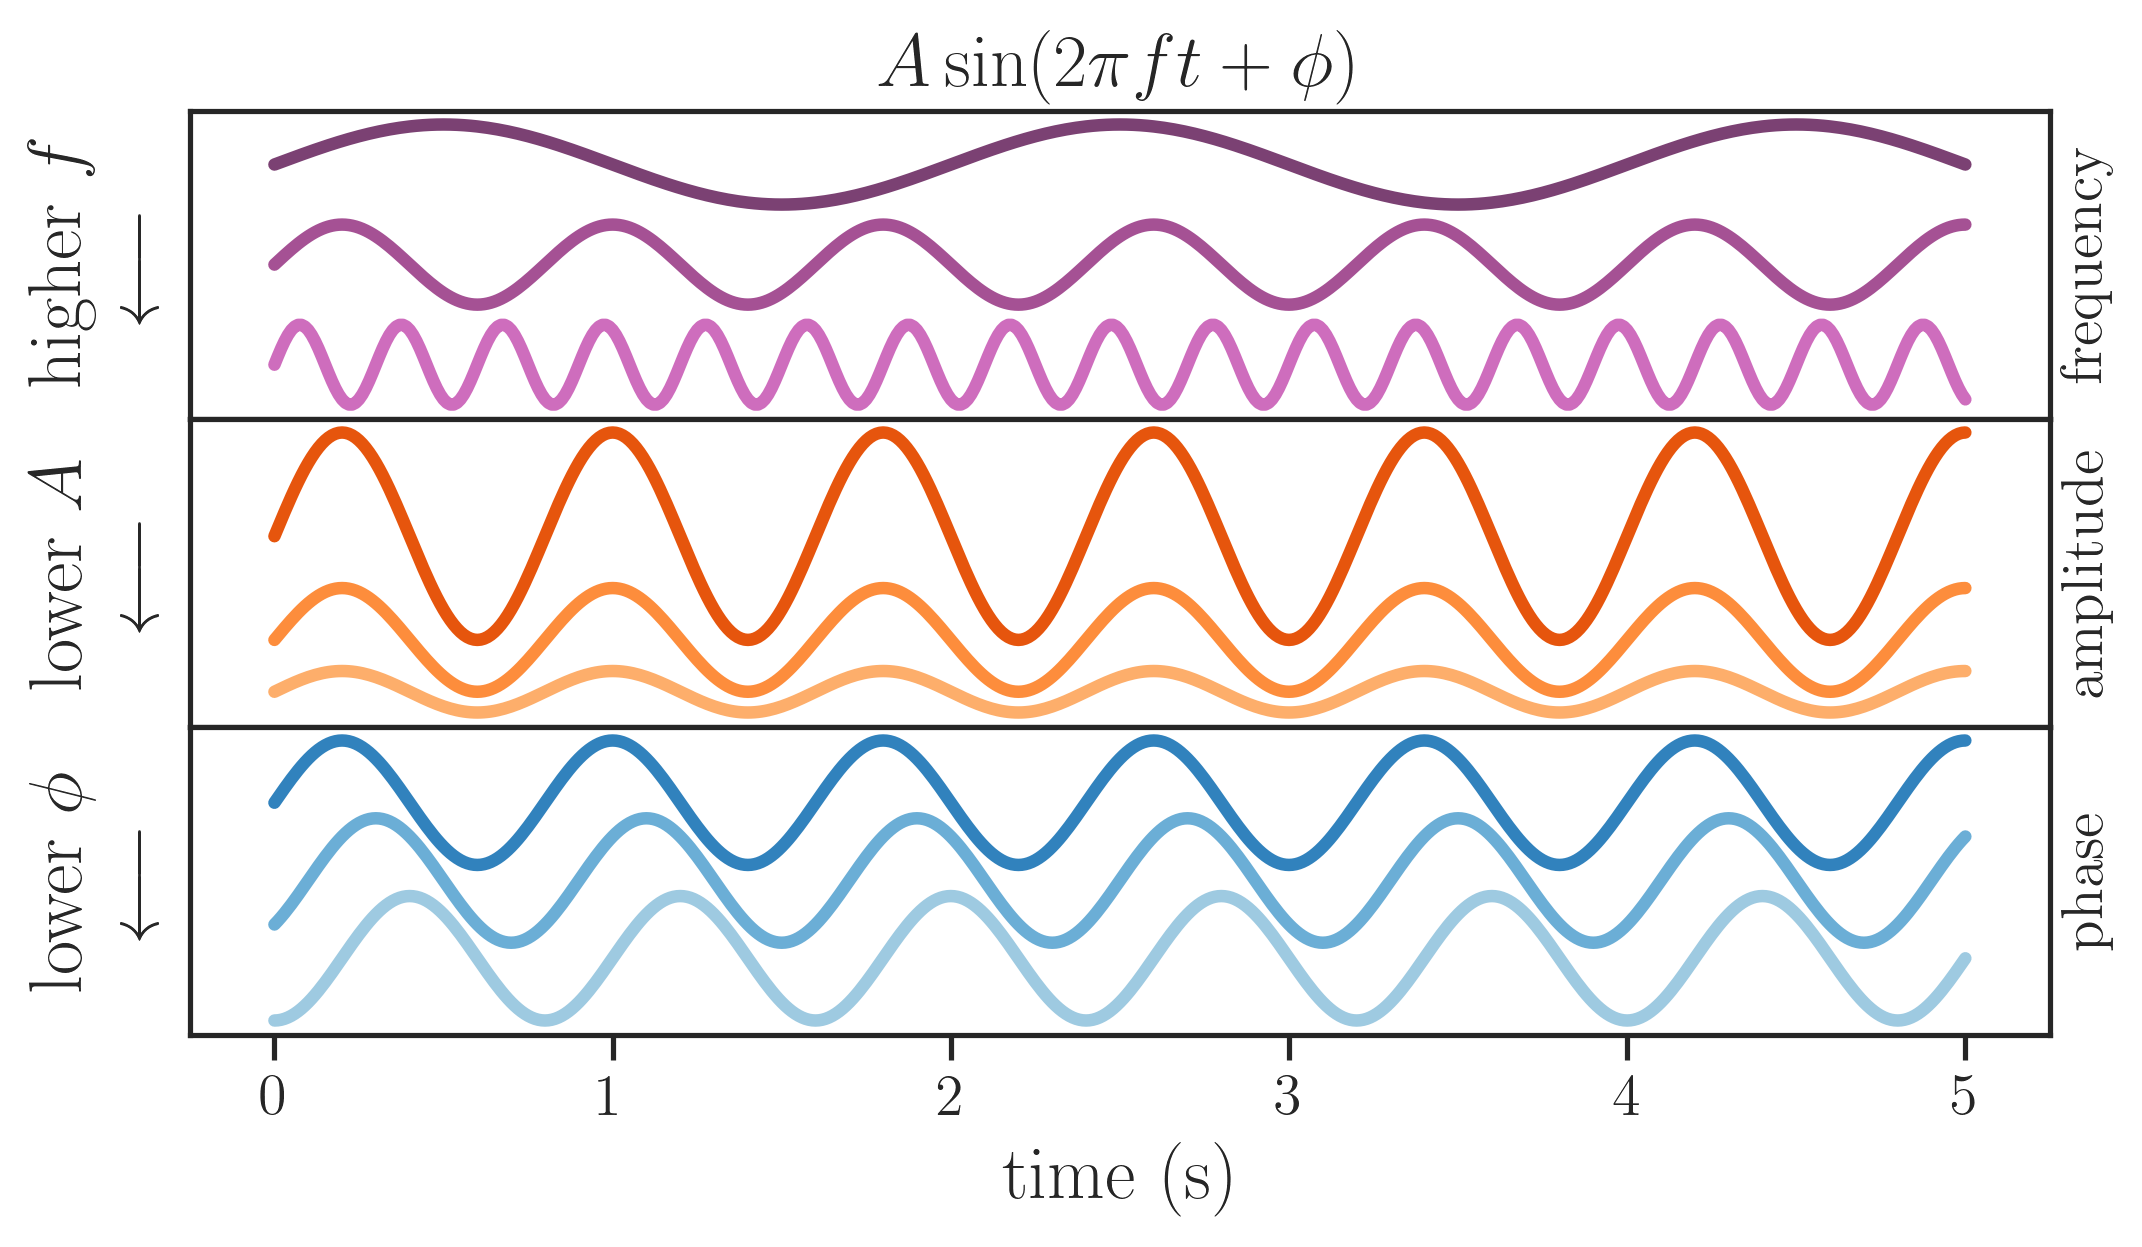
\includegraphics{frequency/sine2.png}

The graph above introduces two new characteristics of a wave, its phase
\(\phi\), and its offset \(B\). A more general description of a sine
wave is

\begin{equation}\protect\hypertarget{eq-sin-Bf-phi}{}{
f(t) = B\sin(2\pi f t + \phi) + B_0.
}\label{eq-sin-Bf-phi}\end{equation}

The offset \(B_0\) moves the wave up and down, while changing the value
of \(\phi\) makes the sine wave move left and right. When the phase
\(\phi=2\pi\), the sine wave will have shifted a full period, and the
resulting wave is identical to the original:

\begin{equation}\protect\hypertarget{eq-sin-Bf-phi-2pi}{}{
B\sin(2\pi f t) = B\sin(2\pi f t + 2\pi).
}\label{eq-sin-Bf-phi-2pi}\end{equation}

All the above can also be said about a cosine, whose general for can be
given as

\begin{equation}\protect\hypertarget{eq-sin-Af-phi}{}{
A\cos(2\pi f t + \phi) + A_0
}\label{eq-sin-Af-phi}\end{equation}

One final point before we jump into the deep waters is that the sine and
cosine functions are related through a simple phase shift:

\[
\cos\left(2\pi f t + \frac{\pi}{2}\right) = \sin\left(2\pi f t\right)
\]

\hypertarget{fouriers-theorem}{%
\section{Fourier's theorem}\label{fouriers-theorem}}

Fourier's theorem states that

\begin{quote}
Any periodic signal is composed of a superposition of pure sine waves,
with suitably chosen amplitudes and phases, whose frequencies are
harmonics of the fundamental frequency of the signal.
\end{quote}

See the following animations to visualize the theorem in action.

\strut \\
Source:
\url{https://en.wikipedia.org/wiki/File:Fourier_series_and_transform.gif}

\strut \\
Source:
\url{https://commons.wikimedia.org/wiki/File:Fourier_synthesis_square_wave_animated.gif}

\strut \\
Source:
\url{https://commons.wikimedia.org/wiki/File:Sawtooth_Fourier_Animation.gif}

\strut \\
Source:
\url{https://commons.wikimedia.org/wiki/File:Continuous_Fourier_transform_of_rect_and_sinc_functions.gif}

\hypertarget{fourier-series}{%
\section{Fourier series}\label{fourier-series}}

\begin{quote}
a periodic function can be described as a sum of sines and cosines.
\end{quote}

\marginnote{\begin{footnotesize}

Not any function, but certainly most functions we will deal with in this
course. The function has to fullful the
\href{https://en.wikipedia.org/wiki/Dirichlet–Jordan_test}{Dirichlet
conditions}

\end{footnotesize}}

The classic examples are usually the square function and the sawtooth
function:

{[}Source: \url{https://www.geogebra.org/m/tkajbzmg}{]}

\url{https://www.geogebra.org/m/k4eq4fkr}

\[
F[x(t)] = F(f) = \int_{-\infty}^{\infty}x(t)e^{-2\pi i f t}dt
\]

\[
f(t) = \int_{-\infty}^{\infty}F(f)e^{2\pi i f t}df
\]

\url{https://dibsmethodsmeetings.github.io/fourier-transforms/}

\url{https://www.jezzamon.com/fourier/index.html}

\hypertarget{filtering}{%
\chapter{filtering}\label{filtering}}

\hypertarget{nyquist-shannon-sampling-theorem}{%
\chapter{Nyquist-Shannon sampling
theorem}\label{nyquist-shannon-sampling-theorem}}

\part{seasonality}

\hypertarget{motivation-7}{%
\chapter{motivation}\label{motivation-7}}

\hypertarget{seasonal-decomposition}{%
\chapter{seasonal decomposition}\label{seasonal-decomposition}}

\begin{Shaded}
\begin{Highlighting}[]
\ImportTok{import}\NormalTok{ numpy }\ImportTok{as}\NormalTok{ np}
\ImportTok{import}\NormalTok{ matplotlib.pyplot }\ImportTok{as}\NormalTok{ plt}
\ImportTok{import}\NormalTok{ pandas }\ImportTok{as}\NormalTok{ pd}
\ImportTok{from}\NormalTok{ pandas.plotting }\ImportTok{import}\NormalTok{ register\_matplotlib\_converters}
\NormalTok{register\_matplotlib\_converters()  }\CommentTok{\# datetime converter for a matplotlib}
\ImportTok{import}\NormalTok{ seaborn }\ImportTok{as}\NormalTok{ sns}
\NormalTok{sns.}\BuiltInTok{set}\NormalTok{(style}\OperatorTok{=}\StringTok{"ticks"}\NormalTok{, font\_scale}\OperatorTok{=}\FloatTok{1.5}\NormalTok{)}
\ImportTok{from}\NormalTok{ statsmodels.tsa.seasonal }\ImportTok{import}\NormalTok{ seasonal\_decompose}
\ImportTok{import}\NormalTok{ matplotlib.dates }\ImportTok{as}\NormalTok{ mdates}
\ImportTok{from}\NormalTok{ matplotlib.dates }\ImportTok{import}\NormalTok{ DateFormatter}
\end{Highlighting}
\end{Shaded}

\hypertarget{trends-in-atmospheric-carbon-dioxide}{%
\section{trends in atmospheric carbon
dioxide}\label{trends-in-atmospheric-carbon-dioxide}}

Mauna Loa CO2 concentration.\\
data from \href{https://gml.noaa.gov/ccgg/trends/data.html}{NOAA}

\begin{Shaded}
\begin{Highlighting}[]
\NormalTok{url }\OperatorTok{=} \StringTok{"https://gml.noaa.gov/webdata/ccgg/trends/co2/co2\_weekly\_mlo.csv"}
\CommentTok{\# df = pd.read\_csv(url, header=47, na\_values=[{-}999.99])}

\CommentTok{\# you can first download, and then read the csv}
\NormalTok{filename }\OperatorTok{=} \StringTok{"co2\_weekly\_mlo.csv"}
\NormalTok{df }\OperatorTok{=}\NormalTok{ pd.read\_csv(filename, header}\OperatorTok{=}\DecValTok{35}\NormalTok{, na\_values}\OperatorTok{=}\NormalTok{[}\OperatorTok{{-}}\FloatTok{999.99}\NormalTok{])}

\NormalTok{df}
\end{Highlighting}
\end{Shaded}

\begin{longtable}[]{@{}llllllllll@{}}
\toprule\noalign{}
& 1974 & 5 & 19 & 1974.3795 & 333.37 & 5.1 & -999.99 & -999.99.1 &
50.39 \\
\midrule\noalign{}
\endhead
\bottomrule\noalign{}
\endlastfoot
0 & 1974 & 5 & 26 & 1974.3986 & 332.95 & 6 & NaN & NaN & 50.05 \\
1 & 1974 & 6 & 2 & 1974.4178 & 332.35 & 5 & NaN & NaN & 49.59 \\
2 & 1974 & 6 & 9 & 1974.4370 & 332.20 & 7 & NaN & NaN & 49.64 \\
3 & 1974 & 6 & 16 & 1974.4562 & 332.37 & 7 & NaN & NaN & 50.06 \\
4 & 1974 & 6 & 23 & 1974.4753 & 331.73 & 5 & NaN & NaN & 49.72 \\
... & ... & ... & ... & ... & ... & ... & ... & ... & ... \\
2565 & 2023 & 7 & 23 & 2023.5575 & 421.28 & 4 & 418.03 & 397.30 &
141.60 \\
2566 & 2023 & 7 & 30 & 2023.5767 & 420.83 & 6 & 418.10 & 396.80 &
141.69 \\
2567 & 2023 & 8 & 6 & 2023.5959 & 420.02 & 6 & 417.36 & 395.65 &
141.41 \\
2568 & 2023 & 8 & 13 & 2023.6151 & 418.98 & 4 & 417.25 & 395.24 &
140.89 \\
2569 & 2023 & 8 & 20 & 2023.6342 & 419.31 & 2 & 416.64 & 395.22 &
141.71 \\
\end{longtable}

\begin{Shaded}
\begin{Highlighting}[]
\NormalTok{df[}\StringTok{\textquotesingle{}date\textquotesingle{}}\NormalTok{] }\OperatorTok{=}\NormalTok{ pd.to\_datetime(df[[}\StringTok{\textquotesingle{}year\textquotesingle{}}\NormalTok{, }\StringTok{\textquotesingle{}month\textquotesingle{}}\NormalTok{, }\StringTok{\textquotesingle{}day\textquotesingle{}}\NormalTok{]])}
\NormalTok{df }\OperatorTok{=}\NormalTok{ df.set\_index(}\StringTok{\textquotesingle{}date\textquotesingle{}}\NormalTok{)}
\NormalTok{df}
\end{Highlighting}
\end{Shaded}

\begin{longtable}[]{@{}llllllllll@{}}
\toprule\noalign{}
& year & month & day & decimal & average & ndays & 1 year ago & 10 years
ago & increase since 1800 \\
date & & & & & & & & & \\
\midrule\noalign{}
\endhead
\bottomrule\noalign{}
\endlastfoot
1974-05-19 & 1974 & 5 & 19 & 1974.3795 & 333.37 & 5 & NaN & NaN &
50.40 \\
1974-05-26 & 1974 & 5 & 26 & 1974.3986 & 332.95 & 6 & NaN & NaN &
50.06 \\
1974-06-02 & 1974 & 6 & 2 & 1974.4178 & 332.35 & 5 & NaN & NaN &
49.60 \\
1974-06-09 & 1974 & 6 & 9 & 1974.4370 & 332.20 & 7 & NaN & NaN &
49.65 \\
1974-06-16 & 1974 & 6 & 16 & 1974.4562 & 332.37 & 7 & NaN & NaN &
50.06 \\
... & ... & ... & ... & ... & ... & ... & ... & ... & ... \\
2022-06-26 & 2022 & 6 & 26 & 2022.4836 & 420.31 & 7 & 418.14 & 395.36 &
138.71 \\
2022-07-03 & 2022 & 7 & 3 & 2022.5027 & 419.73 & 6 & 417.49 & 395.15 &
138.64 \\
2022-07-10 & 2022 & 7 & 10 & 2022.5219 & 419.08 & 6 & 417.25 & 394.59 &
138.52 \\
2022-07-17 & 2022 & 7 & 17 & 2022.5411 & 418.43 & 6 & 417.14 & 394.64 &
138.41 \\
2022-07-24 & 2022 & 7 & 24 & 2022.5603 & 417.84 & 6 & 415.68 & 394.11 &
138.36 \\
\end{longtable}

\begin{Shaded}
\begin{Highlighting}[]
\CommentTok{\# \%matplotlib widget}

\NormalTok{fig, ax }\OperatorTok{=}\NormalTok{ plt.subplots(}\DecValTok{1}\NormalTok{, figsize}\OperatorTok{=}\NormalTok{(}\DecValTok{8}\NormalTok{,}\DecValTok{6}\NormalTok{))}
\NormalTok{ax.plot(df[}\StringTok{\textquotesingle{}average\textquotesingle{}}\NormalTok{])}
\NormalTok{ax.}\BuiltInTok{set}\NormalTok{(xlabel}\OperatorTok{=}\StringTok{"date"}\NormalTok{,}
\NormalTok{       ylabel}\OperatorTok{=}\StringTok{"CO2 concentration (ppm)"}\NormalTok{,}
       \CommentTok{\# ylim=[0, 430],}
\NormalTok{       title}\OperatorTok{=}\StringTok{"Mauna Loa CO2 concentration"}\NormalTok{)}\OperatorTok{;}
\end{Highlighting}
\end{Shaded}

\begin{verbatim}
KeyError: 'average'
\end{verbatim}

\begin{figure}[H]

{\centering \includegraphics{seasonality/seasonal-decomposition_files/figure-pdf/cell-5-output-2.png}

}

\end{figure}

fill missing data. interpolate method: `time'\\
\href{https://thepythonyouneed.com/how-to-interpolate-values-with-pandas/}{interpolation
methods visualized}

\begin{Shaded}
\begin{Highlighting}[]
\NormalTok{df[}\StringTok{\textquotesingle{}co2\textquotesingle{}}\NormalTok{] }\OperatorTok{=}\NormalTok{ (df[}\StringTok{\textquotesingle{}average\textquotesingle{}}\NormalTok{].resample(}\StringTok{"D"}\NormalTok{) }\CommentTok{\#resample daily}
\NormalTok{                          .interpolate(method}\OperatorTok{=}\StringTok{\textquotesingle{}time\textquotesingle{}}\NormalTok{) }\CommentTok{\#interpolate by time}
\NormalTok{            )}
\NormalTok{df}
\end{Highlighting}
\end{Shaded}

\begin{longtable}[]{@{}lllllllllll@{}}
\toprule\noalign{}
& year & month & day & decimal & average & ndays & 1 year ago & 10 years
ago & increase since 1800 & co2 \\
date & & & & & & & & & & \\
\midrule\noalign{}
\endhead
\bottomrule\noalign{}
\endlastfoot
1974-05-19 & 1974 & 5 & 19 & 1974.3795 & 333.37 & 5 & NaN & NaN & 50.40
& 333.37 \\
1974-05-26 & 1974 & 5 & 26 & 1974.3986 & 332.95 & 6 & NaN & NaN & 50.06
& 332.95 \\
1974-06-02 & 1974 & 6 & 2 & 1974.4178 & 332.35 & 5 & NaN & NaN & 49.60 &
332.35 \\
1974-06-09 & 1974 & 6 & 9 & 1974.4370 & 332.20 & 7 & NaN & NaN & 49.65 &
332.20 \\
1974-06-16 & 1974 & 6 & 16 & 1974.4562 & 332.37 & 7 & NaN & NaN & 50.06
& 332.37 \\
... & ... & ... & ... & ... & ... & ... & ... & ... & ... & ... \\
2022-06-26 & 2022 & 6 & 26 & 2022.4836 & 420.31 & 7 & 418.14 & 395.36 &
138.71 & 420.31 \\
2022-07-03 & 2022 & 7 & 3 & 2022.5027 & 419.73 & 6 & 417.49 & 395.15 &
138.64 & 419.73 \\
2022-07-10 & 2022 & 7 & 10 & 2022.5219 & 419.08 & 6 & 417.25 & 394.59 &
138.52 & 419.08 \\
2022-07-17 & 2022 & 7 & 17 & 2022.5411 & 418.43 & 6 & 417.14 & 394.64 &
138.41 & 418.43 \\
2022-07-24 & 2022 & 7 & 24 & 2022.5603 & 417.84 & 6 & 415.68 & 394.11 &
138.36 & 417.84 \\
\end{longtable}

\hypertarget{decompose-data}{%
\section{decompose data}\label{decompose-data}}

\texttt{seasonal\_decompose} returns an object with four components:

\begin{itemize}
\tightlist
\item
  observed: \(Y(t)\)
\item
  trend: \(T(t)\)
\item
  seasonal: \(S(t)\)
\item
  resid: \(e(t)\)
\end{itemize}

Additive model: \[
Y(t) = T(t) + S(t) + e(t)
\]

Multiplicative model: \[
Y(t) = T(t) \times S(t) \times e(t)
\]

\hypertarget{interlude}{%
\subsubsection{Interlude}\label{interlude}}

learn how to use \texttt{zip} in a loop

\begin{Shaded}
\begin{Highlighting}[]
\NormalTok{letters }\OperatorTok{=}\NormalTok{ [}\StringTok{\textquotesingle{}a\textquotesingle{}}\NormalTok{, }\StringTok{\textquotesingle{}b\textquotesingle{}}\NormalTok{, }\StringTok{\textquotesingle{}c\textquotesingle{}}\NormalTok{, }\StringTok{\textquotesingle{}d\textquotesingle{}}\NormalTok{, }\StringTok{\textquotesingle{}e\textquotesingle{}}\NormalTok{]}
\NormalTok{numbers }\OperatorTok{=}\NormalTok{ [}\DecValTok{1}\NormalTok{, }\DecValTok{2}\NormalTok{, }\DecValTok{3}\NormalTok{, }\DecValTok{4}\NormalTok{, }\DecValTok{5}\NormalTok{]}
\CommentTok{\# zip let\textquotesingle{}s us iterate over to lists at the same time}
\ControlFlowTok{for}\NormalTok{ l, n }\KeywordTok{in} \BuiltInTok{zip}\NormalTok{(letters, numbers):}
    \BuiltInTok{print}\NormalTok{(}\SpecialStringTok{f"}\SpecialCharTok{\{}\NormalTok{l}\SpecialCharTok{\}}\SpecialStringTok{ = }\SpecialCharTok{\{}\NormalTok{n}\SpecialCharTok{\}}\SpecialStringTok{"}\NormalTok{)}
\end{Highlighting}
\end{Shaded}

\begin{verbatim}
a = 1
b = 2
c = 3
d = 4
e = 5
\end{verbatim}

Plot each component separately.

\begin{Shaded}
\begin{Highlighting}[]
\CommentTok{\# \%matplotlib widget}

\NormalTok{fig, ax }\OperatorTok{=}\NormalTok{ plt.subplots(}\DecValTok{4}\NormalTok{, }\DecValTok{1}\NormalTok{, figsize}\OperatorTok{=}\NormalTok{(}\DecValTok{8}\NormalTok{,}\DecValTok{6}\NormalTok{), sharex}\OperatorTok{=}\VariableTok{True}\NormalTok{)}
\NormalTok{decomposed\_m }\OperatorTok{=}\NormalTok{ seasonal\_decompose(df[}\StringTok{\textquotesingle{}co2\textquotesingle{}}\NormalTok{], model}\OperatorTok{=}\StringTok{\textquotesingle{}multiplicative\textquotesingle{}}\NormalTok{)}
\NormalTok{decomposed\_a }\OperatorTok{=}\NormalTok{ seasonal\_decompose(df[}\StringTok{\textquotesingle{}co2\textquotesingle{}}\NormalTok{], model}\OperatorTok{=}\StringTok{\textquotesingle{}additive\textquotesingle{}}\NormalTok{)}
\NormalTok{decomposed }\OperatorTok{=}\NormalTok{ decomposed\_m}
\NormalTok{pos }\OperatorTok{=}\NormalTok{ (}\FloatTok{0.5}\NormalTok{, }\FloatTok{0.9}\NormalTok{)}
\NormalTok{components }\OperatorTok{=}\NormalTok{[}\StringTok{"observed"}\NormalTok{, }\StringTok{"trend"}\NormalTok{, }\StringTok{"seasonal"}\NormalTok{, }\StringTok{"resid"}\NormalTok{]}
\NormalTok{colors }\OperatorTok{=}\NormalTok{ [}\StringTok{"tab:blue"}\NormalTok{, }\StringTok{"tab:orange"}\NormalTok{, }\StringTok{"tab:green"}\NormalTok{, }\StringTok{"tab:red"}\NormalTok{]}
\ControlFlowTok{for}\NormalTok{ axx, component, color }\KeywordTok{in} \BuiltInTok{zip}\NormalTok{(ax, components, colors):}
\NormalTok{    data }\OperatorTok{=} \BuiltInTok{getattr}\NormalTok{(decomposed, component)}
\NormalTok{    axx.plot(data, color}\OperatorTok{=}\NormalTok{color)}
\NormalTok{    axx.text(}\OperatorTok{*}\NormalTok{pos, component, bbox}\OperatorTok{=}\BuiltInTok{dict}\NormalTok{(facecolor}\OperatorTok{=}\StringTok{\textquotesingle{}white\textquotesingle{}}\NormalTok{, alpha}\OperatorTok{=}\FloatTok{0.8}\NormalTok{),}
\NormalTok{           transform}\OperatorTok{=}\NormalTok{axx.transAxes, ha}\OperatorTok{=}\StringTok{\textquotesingle{}center\textquotesingle{}}\NormalTok{, va}\OperatorTok{=}\StringTok{\textquotesingle{}top\textquotesingle{}}\NormalTok{)}
\end{Highlighting}
\end{Shaded}

\begin{figure}[H]

{\centering \includegraphics{seasonality/seasonal-decomposition_files/figure-pdf/cell-8-output-1.png}

}

\end{figure}

\begin{Shaded}
\begin{Highlighting}[]
\CommentTok{\# \%matplotlib widget}

\NormalTok{decomposed }\OperatorTok{=}\NormalTok{ decomposed\_m}

\NormalTok{fig, ax }\OperatorTok{=}\NormalTok{ plt.subplots(}\DecValTok{1}\NormalTok{, }\DecValTok{2}\NormalTok{, figsize}\OperatorTok{=}\NormalTok{(}\DecValTok{10}\NormalTok{,}\DecValTok{6}\NormalTok{))}
\NormalTok{ax[}\DecValTok{0}\NormalTok{].plot(df[}\StringTok{\textquotesingle{}co2\textquotesingle{}}\NormalTok{], color}\OperatorTok{=}\StringTok{"tab:blue"}\NormalTok{, label}\OperatorTok{=}\StringTok{"observed"}\NormalTok{)}
\NormalTok{ax[}\DecValTok{0}\NormalTok{].plot(decomposed.trend }\OperatorTok{*}\NormalTok{ decomposed.resid, color}\OperatorTok{=}\StringTok{"tab:orange"}\NormalTok{, label}\OperatorTok{=}\StringTok{"trend*resid"}\NormalTok{)}
\NormalTok{ax[}\DecValTok{0}\NormalTok{].plot(decomposed.trend }\OperatorTok{*}\NormalTok{ decomposed.seasonal, color}\OperatorTok{=}\StringTok{"tab:red"}\NormalTok{, label}\OperatorTok{=}\StringTok{"trend*seasonal"}\NormalTok{)}
\NormalTok{ax[}\DecValTok{0}\NormalTok{].plot(decomposed.trend, color}\OperatorTok{=}\StringTok{"black"}\NormalTok{, label}\OperatorTok{=}\StringTok{"trend"}\NormalTok{)}
\NormalTok{ax[}\DecValTok{0}\NormalTok{].}\BuiltInTok{set}\NormalTok{(ylabel}\OperatorTok{=}\StringTok{"CO$\_2$ concentration (ppm)"}\NormalTok{,}
\NormalTok{          title}\OperatorTok{=}\StringTok{"Mauna Loa CO$\_2$ concentration"}\NormalTok{)}
\NormalTok{ax[}\DecValTok{0}\NormalTok{].legend(frameon}\OperatorTok{=}\VariableTok{False}\NormalTok{)}

\NormalTok{start }\OperatorTok{=} \StringTok{"2000{-}01{-}01"}
\NormalTok{end }\OperatorTok{=} \StringTok{"2003{-}01{-}01"}
\NormalTok{zoom }\OperatorTok{=} \BuiltInTok{slice}\NormalTok{(start, end)}
\NormalTok{ax[}\DecValTok{1}\NormalTok{].plot(df.loc[zoom, }\StringTok{\textquotesingle{}co2\textquotesingle{}}\NormalTok{], color}\OperatorTok{=}\StringTok{"tab:blue"}\NormalTok{, label}\OperatorTok{=}\StringTok{"observed"}\NormalTok{)}
\NormalTok{ax[}\DecValTok{1}\NormalTok{].plot((decomposed.trend }\OperatorTok{*}\NormalTok{ decomposed.resid)[zoom], color}\OperatorTok{=}\StringTok{"tab:orange"}\NormalTok{, label}\OperatorTok{=}\StringTok{"trend*resid"}\NormalTok{)}
\NormalTok{ax[}\DecValTok{1}\NormalTok{].plot((decomposed.trend }\OperatorTok{*}\NormalTok{ decomposed.seasonal)[zoom], color}\OperatorTok{=}\StringTok{"tab:red"}\NormalTok{, label}\OperatorTok{=}\StringTok{"trend*seasonal"}\NormalTok{)}
\NormalTok{ax[}\DecValTok{1}\NormalTok{].plot(decomposed.trend[zoom], color}\OperatorTok{=}\StringTok{"black"}\NormalTok{, label}\OperatorTok{=}\StringTok{"trend"}\NormalTok{)}
\NormalTok{date\_form }\OperatorTok{=}\NormalTok{ DateFormatter(}\StringTok{"\%Y"}\NormalTok{)}
\NormalTok{ax[}\DecValTok{1}\NormalTok{].xaxis.set\_major\_formatter(date\_form)}
\NormalTok{ax[}\DecValTok{1}\NormalTok{].xaxis.set\_major\_locator(mdates.YearLocator(}\DecValTok{1}\NormalTok{))}
\NormalTok{ax[}\DecValTok{1}\NormalTok{].set\_title(}\StringTok{"Components, 2000{-}{-}2003"}\NormalTok{)}\OperatorTok{;}
\end{Highlighting}
\end{Shaded}

\begin{figure}[H]

{\centering \includegraphics{seasonality/seasonal-decomposition_files/figure-pdf/cell-9-output-1.png}

}

\end{figure}

\hypertarget{hilbert-transform}{%
\chapter{Hilbert transform}\label{hilbert-transform}}

\part{rates of change}

\hypertarget{motivation-8}{%
\chapter{motivation}\label{motivation-8}}

\begin{Shaded}
\begin{Highlighting}[]
\ImportTok{import}\NormalTok{ numpy }\ImportTok{as}\NormalTok{ np}
\ImportTok{import}\NormalTok{ matplotlib.pyplot }\ImportTok{as}\NormalTok{ plt}
\ImportTok{import}\NormalTok{ pandas }\ImportTok{as}\NormalTok{ pd}
\ImportTok{import}\NormalTok{ seaborn }\ImportTok{as}\NormalTok{ sns}
\NormalTok{sns.}\BuiltInTok{set}\NormalTok{(style}\OperatorTok{=}\StringTok{"ticks"}\NormalTok{, font\_scale}\OperatorTok{=}\FloatTok{1.5}\NormalTok{)  }\CommentTok{\# white graphs, with large and legible letters}
\OperatorTok{\%}\NormalTok{matplotlib widget}
\end{Highlighting}
\end{Shaded}

\begin{Shaded}
\begin{Highlighting}[]
\NormalTok{filename }\OperatorTok{=} \StringTok{"../archive/data/kinneret\_cleaned.csv"}
\NormalTok{df }\OperatorTok{=}\NormalTok{ pd.read\_csv(filename)}
\NormalTok{df[}\StringTok{\textquotesingle{}date\textquotesingle{}}\NormalTok{] }\OperatorTok{=}\NormalTok{ pd.to\_datetime(df[}\StringTok{\textquotesingle{}date\textquotesingle{}}\NormalTok{], dayfirst}\OperatorTok{=}\VariableTok{True}\NormalTok{)}
\NormalTok{df }\OperatorTok{=}\NormalTok{ df.set\_index(}\StringTok{\textquotesingle{}date\textquotesingle{}}\NormalTok{)}
\NormalTok{df}
\end{Highlighting}
\end{Shaded}

\begin{longtable}[]{@{}ll@{}}
\toprule\noalign{}
& level \\
date & \\
\midrule\noalign{}
\endhead
\bottomrule\noalign{}
\endlastfoot
2023-09-12 & -211.115 \\
2023-09-11 & -211.105 \\
2023-09-10 & -211.095 \\
2023-09-09 & -211.085 \\
2023-09-08 & -211.070 \\
... & ... \\
1966-11-01 & -210.390 \\
1966-10-15 & -210.320 \\
1966-10-01 & -210.270 \\
1966-09-15 & -210.130 \\
1966-09-01 & -210.020 \\
\end{longtable}

\begin{Shaded}
\begin{Highlighting}[]
\NormalTok{fig, ax }\OperatorTok{=}\NormalTok{ plt.subplots()}
\NormalTok{ax.plot(df[}\StringTok{\textquotesingle{}level\textquotesingle{}}\NormalTok{], color}\OperatorTok{=}\StringTok{"tab:blue"}\NormalTok{)}
\NormalTok{ax.}\BuiltInTok{set}\NormalTok{(title}\OperatorTok{=}\StringTok{"Kinneret Level"}\NormalTok{,}
\NormalTok{       ylabel}\OperatorTok{=}\StringTok{"level (m)"}\NormalTok{)}
\NormalTok{plt.gcf().autofmt\_xdate()  }\CommentTok{\# makes slanted dates}
\end{Highlighting}
\end{Shaded}

\begin{figure}[H]

{\centering \includegraphics{rates-of-change/motivation_files/figure-pdf/cell-4-output-1.png}

}

\end{figure}

The data seems ok, until we take a closer look. Data points are not
evenly spaced in time.

\begin{Shaded}
\begin{Highlighting}[]
\NormalTok{fig, ax }\OperatorTok{=}\NormalTok{ plt.subplots()}
\NormalTok{ax.plot(df.loc[}\StringTok{"1993"}\NormalTok{:}\StringTok{"1995"}\NormalTok{, }\StringTok{\textquotesingle{}level\textquotesingle{}}\NormalTok{], color}\OperatorTok{=}\StringTok{"tab:blue"}\NormalTok{, marker}\OperatorTok{=}\StringTok{"o"}\NormalTok{)}
\NormalTok{ax.}\BuiltInTok{set}\NormalTok{(title}\OperatorTok{=}\StringTok{"Dead Sea Level"}\NormalTok{,}
\NormalTok{       ylabel}\OperatorTok{=}\StringTok{"level (m)"}\NormalTok{)}
\NormalTok{plt.gcf().autofmt\_xdate()  }\CommentTok{\# makes slanted dates}
\end{Highlighting}
\end{Shaded}

\begin{verbatim}
/var/folders/c3/7hp0d36n6vv8jc9hm2440__00000gn/T/ipykernel_3777/934261896.py:2: FutureWarning: Value based partial slicing on non-monotonic DatetimeIndexes with non-existing keys is deprecated and will raise a KeyError in a future Version.
  ax.plot(df.loc["1993":"1995", 'level'], color="tab:blue", marker="o")
\end{verbatim}

\begin{figure}[H]

{\centering \includegraphics{rates-of-change/motivation_files/figure-pdf/cell-5-output-2.png}

}

\end{figure}

We can resample by day (a much higher rate than the original), and
linearly interpolate:

\begin{Shaded}
\begin{Highlighting}[]
\NormalTok{df2 }\OperatorTok{=}\NormalTok{ df[}\StringTok{\textquotesingle{}level\textquotesingle{}}\NormalTok{].resample(}\StringTok{\textquotesingle{}D\textquotesingle{}}\NormalTok{).interpolate(}\StringTok{\textquotesingle{}time\textquotesingle{}}\NormalTok{).to\_frame()}
\NormalTok{df2[}\StringTok{\textquotesingle{}level\_sm\textquotesingle{}}\NormalTok{] }\OperatorTok{=}\NormalTok{ df2[}\StringTok{\textquotesingle{}level\textquotesingle{}}\NormalTok{].rolling(}\StringTok{\textquotesingle{}30D\textquotesingle{}}\NormalTok{, center}\OperatorTok{=}\VariableTok{True}\NormalTok{).mean()}
\NormalTok{df3 }\OperatorTok{=}\NormalTok{ df2[}\StringTok{\textquotesingle{}level\textquotesingle{}}\NormalTok{].resample(}\StringTok{\textquotesingle{}W\textquotesingle{}}\NormalTok{).mean().to\_frame()}
\end{Highlighting}
\end{Shaded}

\begin{Shaded}
\begin{Highlighting}[]
\NormalTok{fig, ax }\OperatorTok{=}\NormalTok{ plt.subplots()}
\NormalTok{ax.plot(df2.loc[}\StringTok{"1993"}\NormalTok{:}\StringTok{"1995"}\NormalTok{, }\StringTok{\textquotesingle{}level\_sm\textquotesingle{}}\NormalTok{],}
\NormalTok{        color}\OperatorTok{=}\StringTok{"tab:red"}\NormalTok{,}
\NormalTok{        label}\OperatorTok{=}\StringTok{"daily resapled"}\NormalTok{)}
\NormalTok{ax.plot(df3.loc[}\StringTok{"1993"}\NormalTok{:}\StringTok{"1995"}\NormalTok{, }\StringTok{\textquotesingle{}level\textquotesingle{}}\NormalTok{],}
\NormalTok{        color}\OperatorTok{=}\StringTok{"black"}\NormalTok{,}
\NormalTok{        label}\OperatorTok{=}\StringTok{"daily resapled"}\NormalTok{)}
\NormalTok{ax.plot(df2.loc[}\StringTok{"1993"}\NormalTok{:}\StringTok{"1995"}\NormalTok{, }\StringTok{\textquotesingle{}level\textquotesingle{}}\NormalTok{],}
\NormalTok{        color}\OperatorTok{=}\StringTok{"tab:orange"}\NormalTok{,}
\NormalTok{        label}\OperatorTok{=}\StringTok{"daily resapled"}\NormalTok{)}
\NormalTok{ax.plot(df.loc[}\StringTok{"1993"}\NormalTok{:}\StringTok{"1995"}\NormalTok{, }\StringTok{\textquotesingle{}level\textquotesingle{}}\NormalTok{],}
\NormalTok{        color}\OperatorTok{=}\StringTok{"tab:blue"}\NormalTok{,}
\NormalTok{        marker}\OperatorTok{=}\StringTok{"o"}\NormalTok{,}
\NormalTok{        linestyle}\OperatorTok{=}\StringTok{"None"}\NormalTok{,}
\NormalTok{        label}\OperatorTok{=}\StringTok{"original"}\NormalTok{)}
\NormalTok{ax.}\BuiltInTok{set}\NormalTok{(title}\OperatorTok{=}\StringTok{"Dead Sea Level"}\NormalTok{,}
\NormalTok{       ylabel}\OperatorTok{=}\StringTok{"level (m)"}\NormalTok{)}
\NormalTok{plt.gcf().autofmt\_xdate()  }\CommentTok{\# makes slanted dates}
\NormalTok{ax.legend(frameon}\OperatorTok{=}\VariableTok{False}\NormalTok{)}
\end{Highlighting}
\end{Shaded}

\begin{verbatim}
/var/folders/c3/7hp0d36n6vv8jc9hm2440__00000gn/T/ipykernel_3777/2583247388.py:11: FutureWarning: Value based partial slicing on non-monotonic DatetimeIndexes with non-existing keys is deprecated and will raise a KeyError in a future Version.
  ax.plot(df.loc["1993":"1995", 'level'],
\end{verbatim}

\begin{verbatim}
<matplotlib.legend.Legend at 0x7fa71e8b0bb0>
\end{verbatim}

\begin{figure}[H]

{\centering \includegraphics{rates-of-change/motivation_files/figure-pdf/cell-7-output-3.png}

}

\end{figure}

\begin{Shaded}
\begin{Highlighting}[]
\NormalTok{df2[}\StringTok{\textquotesingle{}naive\textquotesingle{}}\NormalTok{] }\OperatorTok{=}\NormalTok{ df2[}\StringTok{\textquotesingle{}level\textquotesingle{}}\NormalTok{].diff()}
\NormalTok{df2[}\StringTok{\textquotesingle{}gradient\textquotesingle{}}\NormalTok{] }\OperatorTok{=}\NormalTok{ np.gradient(df2[}\StringTok{\textquotesingle{}level\textquotesingle{}}\NormalTok{])}

\NormalTok{df3[}\StringTok{\textquotesingle{}naive\textquotesingle{}}\NormalTok{] }\OperatorTok{=}\NormalTok{ df3[}\StringTok{\textquotesingle{}level\textquotesingle{}}\NormalTok{].diff()}
\NormalTok{df3[}\StringTok{\textquotesingle{}gradient\textquotesingle{}}\NormalTok{] }\OperatorTok{=}\NormalTok{ np.gradient(df3[}\StringTok{\textquotesingle{}level\textquotesingle{}}\NormalTok{])}
\end{Highlighting}
\end{Shaded}

\begin{Shaded}
\begin{Highlighting}[]
\NormalTok{fig, ax }\OperatorTok{=}\NormalTok{ plt.subplots()}
\NormalTok{ax.plot(df3.loc[}\StringTok{"1980"}\NormalTok{:}\StringTok{"2020"}\NormalTok{, }\StringTok{\textquotesingle{}naive\textquotesingle{}}\NormalTok{], color}\OperatorTok{=}\StringTok{"tab:blue"}\NormalTok{)}
\NormalTok{ax.plot(df3.loc[}\StringTok{"1980"}\NormalTok{:}\StringTok{"2020"}\NormalTok{, }\StringTok{\textquotesingle{}gradient\textquotesingle{}}\NormalTok{], color}\OperatorTok{=}\StringTok{"tab:red"}\NormalTok{)}
\NormalTok{ax.}\BuiltInTok{set}\NormalTok{(title}\OperatorTok{=}\StringTok{"Dead Sea Level"}\NormalTok{,}
\NormalTok{       ylabel}\OperatorTok{=}\StringTok{"level (m)"}\NormalTok{)}
\end{Highlighting}
\end{Shaded}

\begin{verbatim}
[Text(0.5, 1.0, 'Dead Sea Level'), Text(0, 0.5, 'level (m)')]
\end{verbatim}

\begin{figure}[H]

{\centering 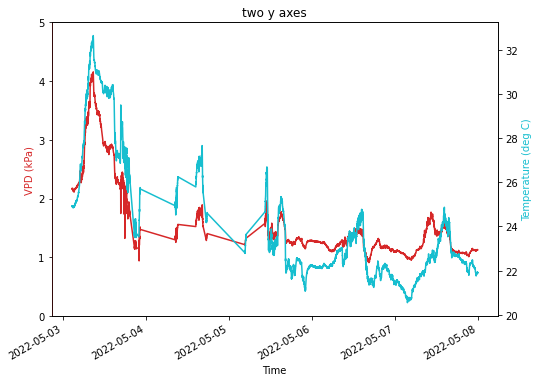
\includegraphics{rates-of-change/motivation_files/figure-pdf/cell-9-output-2.png}

}

\end{figure}

\begin{Shaded}
\begin{Highlighting}[]
\NormalTok{df3 }\OperatorTok{=}\NormalTok{ df2[}\StringTok{"level"}\NormalTok{].rolling(}\StringTok{\textquotesingle{}365.24D\textquotesingle{}}\NormalTok{, center}\OperatorTok{=}\VariableTok{True}\NormalTok{).mean().to\_frame()}
\end{Highlighting}
\end{Shaded}

\begin{Shaded}
\begin{Highlighting}[]
\NormalTok{fig, ax }\OperatorTok{=}\NormalTok{ plt.subplots()}
\NormalTok{ax.plot(df3.loc[}\StringTok{"1980"}\NormalTok{:}\StringTok{"2020"}\NormalTok{, }\StringTok{\textquotesingle{}level\textquotesingle{}}\NormalTok{], color}\OperatorTok{=}\StringTok{"tab:blue"}\NormalTok{)}
\NormalTok{ax.}\BuiltInTok{set}\NormalTok{(title}\OperatorTok{=}\StringTok{"Dead Sea Level"}\NormalTok{,}
\NormalTok{       ylabel}\OperatorTok{=}\StringTok{"level (m)"}\NormalTok{)}
\end{Highlighting}
\end{Shaded}

\begin{verbatim}
[Text(0.5, 1.0, 'Dead Sea Level'), Text(0, 0.5, 'level (m)')]
\end{verbatim}

\begin{figure}[H]

{\centering 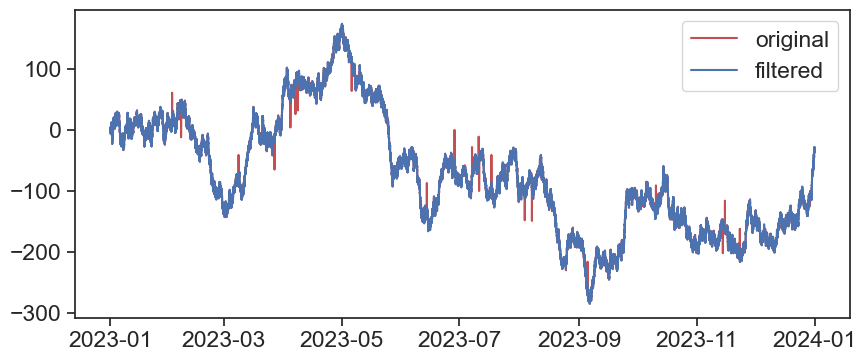
\includegraphics{rates-of-change/motivation_files/figure-pdf/cell-11-output-2.png}

}

\end{figure}

\hypertarget{derivatives}{%
\chapter{derivatives}\label{derivatives}}

\hypertarget{finite-differences}{%
\chapter{finite differences}\label{finite-differences}}

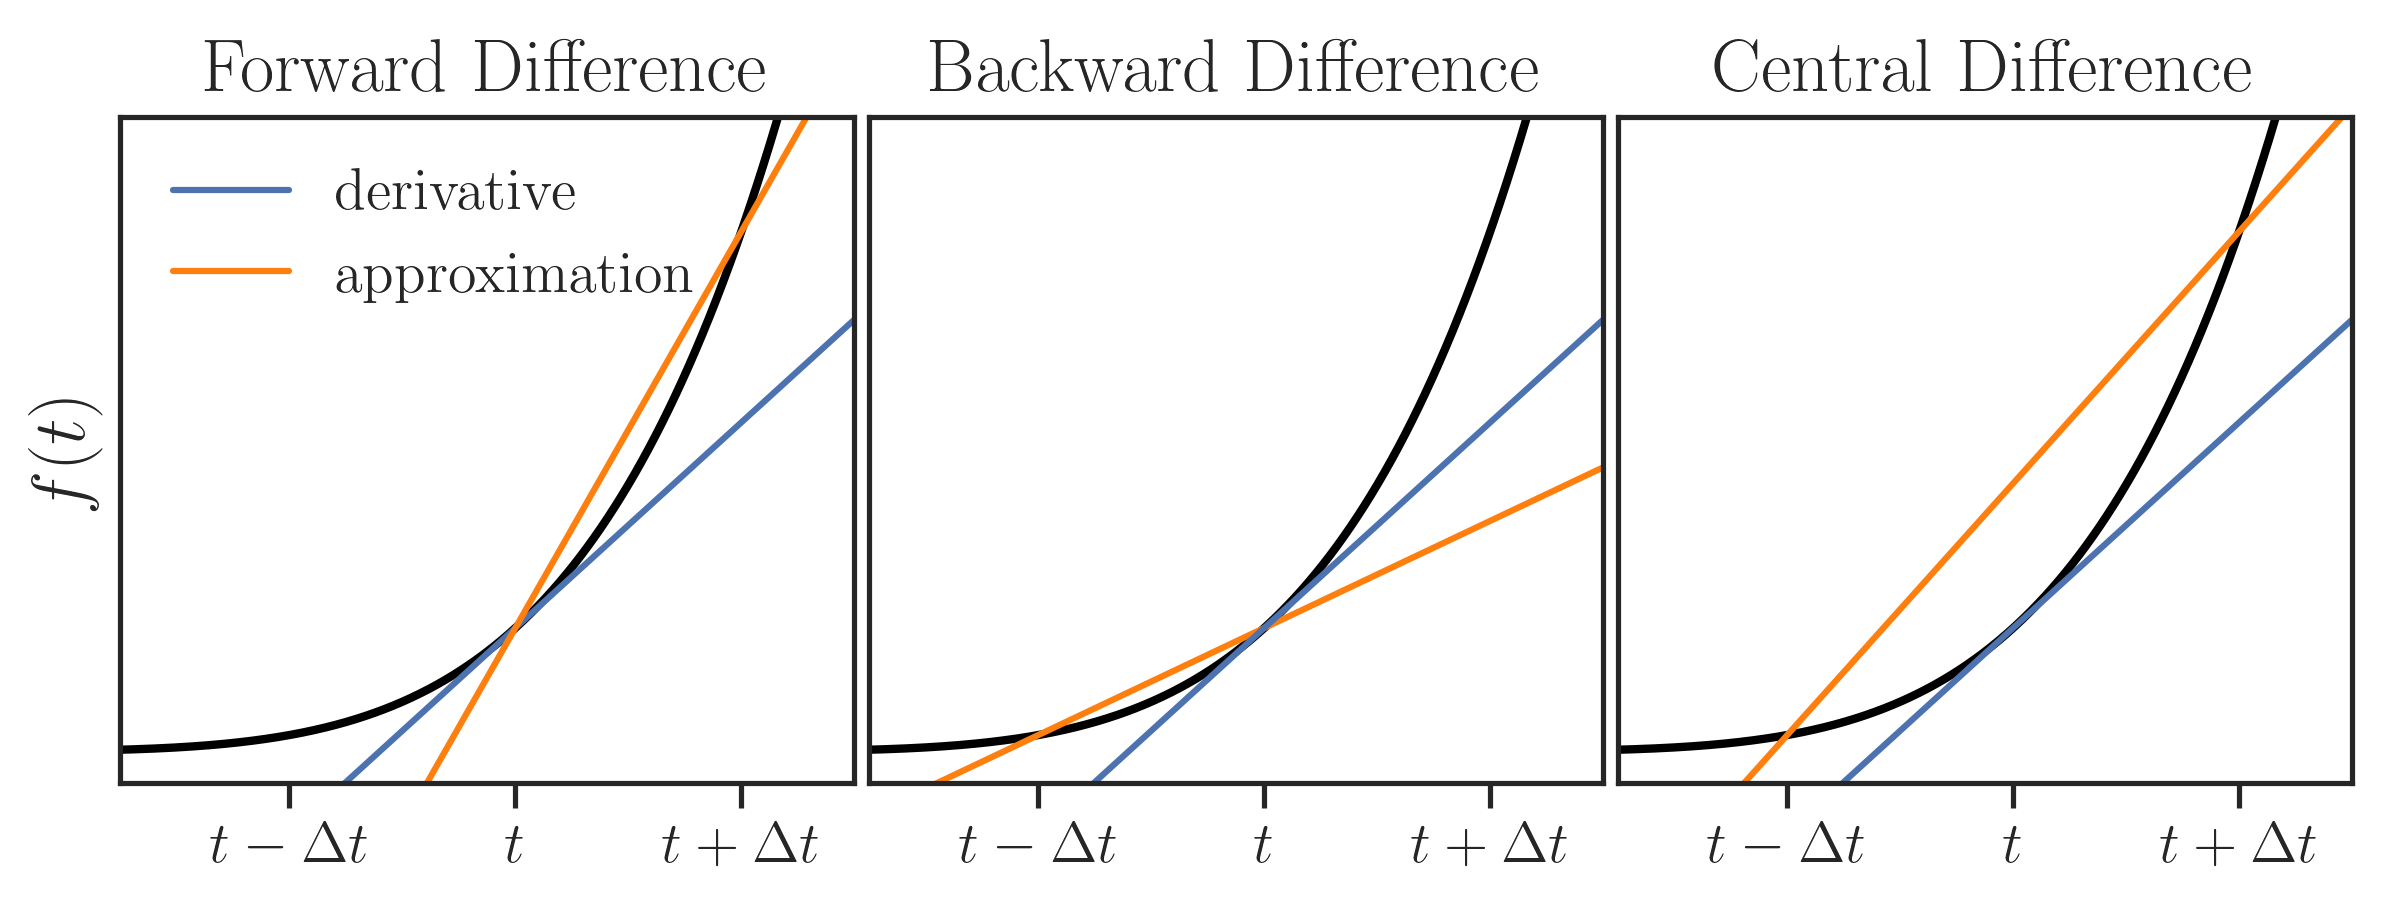
\includegraphics{rates-of-change/central_diff.png}

Definition of a \textbf{derivative}:

\[
\underbrace{\dot{f} = f'(t) = \frac{df(t)}{dt}}_{\text{same thing}} = \lim_{\Delta t \rightarrow 0} \frac{f(t+\Delta t) - f(t)}{\Delta t}.
\]

Numerically, we can approximate the derivative \(f'(t)\) of a time
series \(f(t)\) as

\begin{equation}\protect\hypertarget{eq-tpfdf}{}{
\frac{df(t)}{dt} = \frac{f(t+\Delta t) - f(t)}{\Delta t} + \mathcal{O}(\Delta t).
}\label{eq-tpfdf}\end{equation}

\marginnote{\begin{footnotesize}

The expression \(\mathcal{O}(\Delta t)\) means that the error associated
with the approximation is proportional to \(\Delta t\). This is called
\href{https://en.wikipedia.org/wiki/Big_O_notation}{``Big O notation''}.

\end{footnotesize}}

The expression above is called the \emph{two-point forward difference
formula}. Likewise, we can define the \emph{two-point backward
difference formula}:

\begin{equation}\protect\hypertarget{eq-tpbdf}{}{
\frac{df(t)}{dt} = \frac{f(t) - f(t-\Delta t)}{\Delta t} + \mathcal{O}(\Delta t).
}\label{eq-tpbdf}\end{equation}

If we sum together Equation~\ref{eq-tpfdf} and Equation~\ref{eq-tpbdf}
we get:

\begin{equation}\protect\hypertarget{eq-sum}{}{
\begin{aligned}
2\frac{df(t)}{dt} &= \frac{f(t+\Delta t) - \cancel{f(t)}}{\Delta t} + \frac{\cancel{f(t)} - f(t-\Delta t)}{\Delta t} \\
 &= \frac{f(t+\Delta t) - f(t-\Delta t)}{\Delta t}.
\end{aligned}
}\label{eq-sum}\end{equation}

Dividing both sides by 2 gives the \emph{two-point central difference
formula}:

\begin{equation}\protect\hypertarget{eq-twcdf}{}{
\frac{df(t)}{dt} = \frac{f(t+\Delta t) - f(t-\Delta t)}{2\Delta t} + \mathcal{O}(\Delta t^2). 
}\label{eq-twcdf}\end{equation}

Two things are worth mentioning about the approximation above:

\begin{enumerate}
\def\labelenumi{\arabic{enumi}.}
\tightlist
\item
  it is balanced, that is, there is no preference of the future over the
  past.
\item
  its error is proportional to \(\Delta t^2\), it is a lot more precise
  than the unbalanced approximations :)
\end{enumerate}

\marginnote{\begin{footnotesize}

To understand why the error is proportional to \(\Delta t^2\), one can
subtract the Taylor expansion of \(f(t-\Delta t)\) from the Taylor
expansion of \(f(t+\Delta t)\).
\href{https://home.cc.umanitoba.ca/~farhadi/Math2120/Numerical\%20Differentiation.pdf}{See
this, pages 3 and 4.}

\end{footnotesize}}

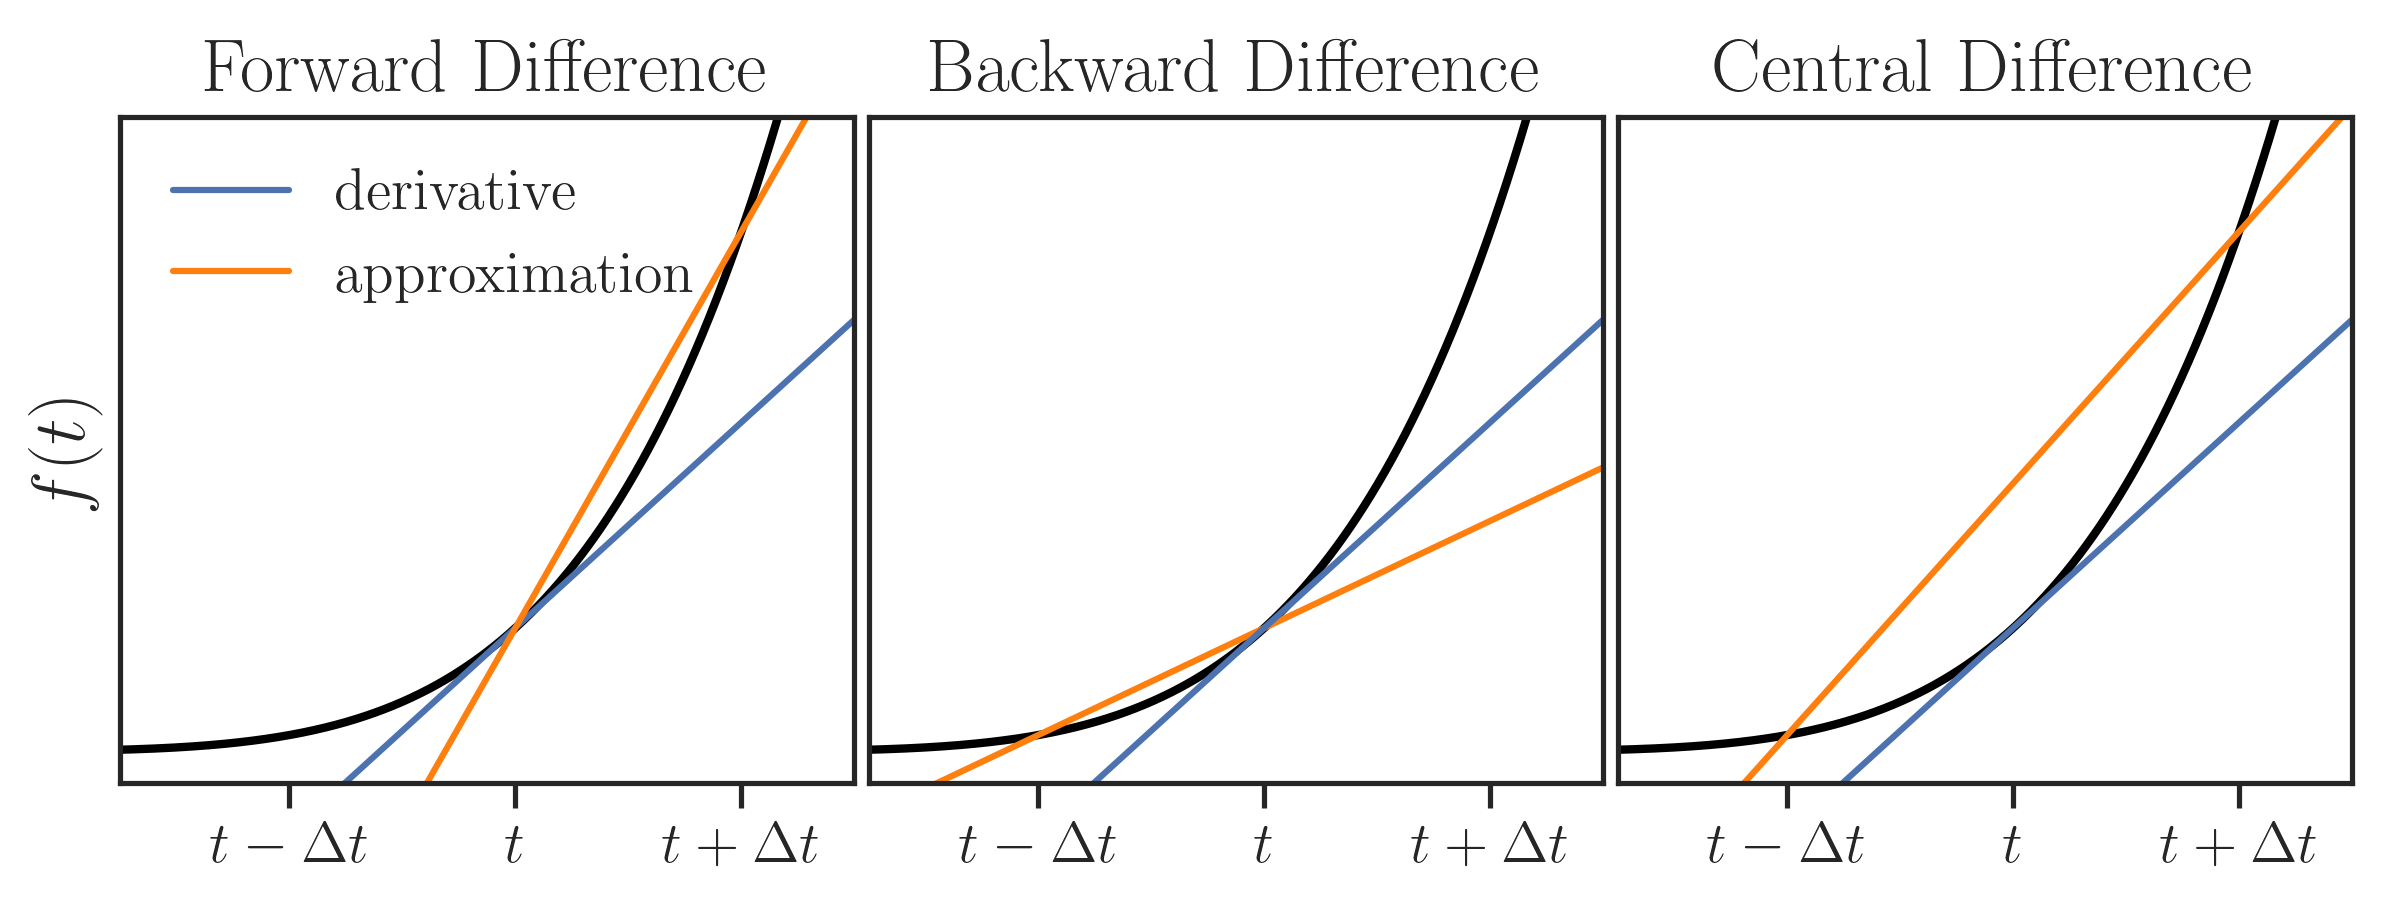
\includegraphics{rates-of-change/central_diff.png}

The function
\href{https://numpy.org/doc/stable/reference/generated/numpy.gradient.html}{\texttt{np.gradient}}
calculates the derivative using the central difference for points in the
interior of the array, and uses the forward (backward) difference for
the derivative at the beginning (end) of the array.

\marginnote{\begin{footnotesize}

The ``gradient'' usually refers to a first derivative with respect to
space, and it is denoted as \(\nabla f(x)=\frac{df(x)}{dx}\). However,
it doesn't really matter if we call the independent variable \(x\) or
\(t\), the derivative operator is exactly the same.

\end{footnotesize}}

Check out this
\href{https://gist.github.com/astrojuanlu/e4d47fec5d94d2224762a61680419eb2}{nice
example}.

\hypertarget{fourier-based-derivatives}{%
\chapter{Fourier-based derivatives}\label{fourier-based-derivatives}}

This tutorial is based on Pelliccia (2019).

nice trick:
\url{https://math.stackexchange.com/questions/430858/fourier-transform-of-derivative}

\hypertarget{loess-based-derivatives}{%
\chapter{LOESS-based derivatives}\label{loess-based-derivatives}}

\part{forecasting}

\hypertarget{motivation-9}{%
\chapter{motivation}\label{motivation-9}}

\hypertarget{arima}{%
\chapter{ARIMA}\label{arima}}

\part{assignments}

\hypertarget{assignment-1}{%
\chapter{assignment 1}\label{assignment-1}}

This assignment comes right after the first session, where we discussed
resampling. Read the whole instructions.

\hypertarget{task}{%
\section{Task}\label{task}}

Go to the \href{https://ims.gov.il/en/data_gov}{IMS website}, and choose
another weather station we have not worked with yet. Download 10-minute
data for a full year, any year.

\textbf{Make 3 graphs:}

\begin{enumerate}
\def\labelenumi{\arabic{enumi}.}
\tightlist
\item
  Daily maximum humidity. Bonus: add another line to the graph, the
  daily minimum humidity.
\item
  The number of rainy dais for each month
\item
  For each day of the year, show the number of hours when global solar
  radiation was above, on average, the threshold 10 W/m\(^2\). Now add
  another line, for the threshold 500 W/m\(^2\).
\end{enumerate}

\textbf{Make 5 more graphs} (total of 8 graphs) of whatever you find
interesting. You have the liberty to explore various facets of your
dataset that capture your interest. It's essential, however, to maintain
a focus on resampling. Each of your plots should effectively showcase
and emphasize different aspects or techniques of resampling in your data
analysis. To ensure diversity in your visualizations, avoid repetitive
themes; for instance, if your first plot illustrates daily wind speed,
then your second plot should not simply be a monthly resampling of wind
speed. Aim for variety and innovation in each plot to fully explore the
potential of resampling in data visualization.

You must download this Jupyter Notebook template. Create a zip file with
your Jupyter notebook and with the \texttt{.csv} you used. Upload this
zip file to the moodle task we created.

\hypertarget{guidelines}{%
\section{Guidelines}\label{guidelines}}

\begin{enumerate}
\def\labelenumi{\arabic{enumi}.}
\tightlist
\item
  Always name the axes and add units when relevant.
\item
  Always give a title to the plot.
\item
  Make sure that all axis tick labels (the numbers/dates on the axes)
  are readable.
\item
  Include a legend if you have multiple lines, colors, or groups.
\item
  Use appropriate scales for the axes (linear, logarithmic, etc.)
  depending on the data's nature.
\item
  Ensure that the plot is adequately sized for all elements to be clear
  and visible.
\item
  Choose colors and markers that are distinguishable, especially for
  plots with multiple elements.
\item
  If applicable, include error bars to indicate the variability or
  uncertainty in the data.
\item
  Use grid lines sparingly; they should not overshadow the data.
\end{enumerate}

\hypertarget{evaluation}{%
\section{Evaluation}\label{evaluation}}

All your assignments will be evaluated according to the following
criteria:

\begin{itemize}
\tightlist
\item
  Presentation. How the graphs look, labels, general organization,
  markdown, clean code.
\item
  Discussion. This is where you explain what you did, what you found
  out, etc.
\item
  Depth of analysis. You can analyze/explore the data with different
  levels of complexity, this is where we take that into consideration.
\item
  Replicability: Your code runs flawlessly.
\item
  Code commenting. Explain in your code what you are doing, this is good
  for everyone, especially for yourself!
\item
  Bonus: for originality, creative problem solving, or notable analysis.
\end{itemize}

\hypertarget{assignment-2}{%
\chapter{assignment 2}\label{assignment-2}}

\hypertarget{final-assignment}{%
\chapter{final assignment}\label{final-assignment}}

\bookmarksetup{startatroot}

\hypertarget{technical-stuff}{%
\chapter{technical stuff}\label{technical-stuff}}

\hypertarget{operating-systems}{%
\section{operating systems}\label{operating-systems}}

I recommend working with UNIX-based operating systems (MacOS or Linux).
Everything is easier.

If you use Windows, consider
\href{https://learn.microsoft.com/en-us/windows/wsl/install}{installing
Linux on Windows with WSL}.

\hypertarget{software}{%
\section{software}\label{software}}

\href{https://www.anaconda.com/download}{Anaconda's Python distribution}

\href{https://code.visualstudio.com/download}{VSCode}

\hypertarget{python-packages}{%
\section{python packages}\label{python-packages}}

\href{https://engineering.fb.com/2021/06/21/open-source/kats/}{Kats ---
a one-stop shop for time series analysis}\\
Developed by Meta

\href{https://www.statsmodels.org/stable/}{statsmodels} statsmodels is a
Python package that provides a complement to scipy for statistical
computations including descriptive statistics and estimation and
inference for statistical models.

\href{https://ydata-profiling.ydata.ai/docs/master/pages/use_cases/time_series_datasets.html}{ydata-profiling}\\
Quick Exploratory Data Analysis on time-series data.
\href{https://towardsdatascience.com/how-to-do-an-eda-for-time-series-cbb92b3b1913}{Read
also this}.

\bookmarksetup{startatroot}

\hypertarget{sources}{%
\chapter*{sources}\label{sources}}
\addcontentsline{toc}{chapter}{sources}

\markboth{sources}{sources}

\hypertarget{books}{%
\section*{books}\label{books}}
\addcontentsline{toc}{section}{books}

\markright{books}

\href{https://www.data-to-viz.com}{from Data to Viz}

\href{https://clauswilke.com/dataviz/}{Fundamentals of Data
Visualization, by Claus O. Wilke}

\href{https://soilwater.github.io/pynotes-agriscience/intro.html}{PyNotes
in Agriscience}

\href{https://otexts.com/fpp3/}{Forecasting: Principles and Practice
(3rd ed), by Rob J Hyndman and George Athanasopoulos}

\href{https://github.com/erykml/Python-for-Finance-Cookbook-2E}{Python
for Finance Cookbook 2nd Edition - Code Repository}

\href{https://huji.primo.exlibrisgroup.com/permalink/972HUJI_INST/10ptda2/alma9920842016603701}{Practical
time series analysis,: prediction with statistics and machine learning,
by Aileen Nielsen}\\
The online edition of this book is available for Hebrew University staff
and students.

\href{https://huji.primo.exlibrisgroup.com/permalink/972HUJI_INST/10ptda2/alma9921049267803701}{Time
series analysis with Python cookbook : practical recipes for exploratory
data analysis, data preparation, forecasting, and model evaluation, by
Tarek A. Atwan}\\
The online edition of this book is available for Hebrew University staff
and students.

\href{https://huji.primo.exlibrisgroup.com/permalink/972HUJI_INST/10ptda2/alma9920845706703701}{Hands-on
Time Series Analysis with Python: From Basics to Bleeding Edge
Techniques, by B V Vishwas, Ashish Patel}\\
The online edition of this book is available for Hebrew University staff
and students.

\hypertarget{videos}{%
\section*{videos}\label{videos}}
\addcontentsline{toc}{section}{videos}

\markright{videos}

\href{https://learning.oreilly.com/videos/times-series-analysis/9780136944515/}{Times
Series Analysis for Everyone, by Bruno Goncalves}\\
This series is available for Hebrew University staff and students.

\href{https://learning.oreilly.com/videos/time-series-analysis/00000G9DZPO7DJKE/}{Time
Series Analysis with Pandas, by Joshua Malina} This video is available
for Hebrew University staff and students.

\hypertarget{references}{%
\section*{references}\label{references}}
\addcontentsline{toc}{section}{references}

\markright{references}

\hypertarget{refs}{}
\begin{CSLReferences}{1}{0}
\leavevmode\vadjust pre{\hypertarget{ref-atwan2022time}{}}%
Atwan, Tarek A. 2022. \emph{Time Series Analysis with Python Cookbook:
Practical Recipes for Exploratory Data Analysis, Data Preparation,
Forecasting, and Model Evaluation}. Packt.

\leavevmode\vadjust pre{\hypertarget{ref-eilers2003perfect}{}}%
Eilers, Paul HC. 2003. {``A Perfect Smoother.''} \emph{Analytical
Chemistry} 75 (14): 3631--36. \url{https://doi.org/10.1021/ac034173t}.

\leavevmode\vadjust pre{\hypertarget{ref-Andy_McDonald_2022}{}}%
McDonald, Andy. 2022. {``Creating Boxplots with the Seaborn Python
Library.''} \emph{Medium}. Towards Data Science.
\url{https://towardsdatascience.com/creating-boxplots-with-the-seaborn-python-library-f0c20f09bd57}.

\leavevmode\vadjust pre{\hypertarget{ref-pelliccia2019fourier}{}}%
Pelliccia, Daniel. 2019. {``Fourier Spectral Smoothing Method.''} 2019.
\url{https://nirpyresearch.com/fourier-spectral-smoothing-method/}.

\leavevmode\vadjust pre{\hypertarget{ref-Ou_Zhang_2020}{}}%
Zhang, Ou. 2020. {``Outliers-Part 3:outliers in Regression.''}
ouzhang.me.
\url{https://ouzhang.me/blog/outlier-series/outliers-part3/}.

\end{CSLReferences}

\bookmarksetup{startatroot}

\hypertarget{stuff}{%
\chapter*{stuff}\label{stuff}}
\addcontentsline{toc}{chapter}{stuff}

\markboth{stuff}{stuff}

Hey! What are you doing here? This page is not meant for you 😜

\begin{itemize}
\tightlist
\item
  This is not a coding course. Neither a programming course. Our goal is
  to learn how to \textbf{think} about time series. Of course, we want
  to tell the computer how to do stuff, and that requires programming.
\item
  ``How do you do?'' \emph{How do you do what?!}\\
  \emph{Welche Sprachen sprechen Sie?}\\
  First do, then get use to it.\\
  Once you got used to doing, go back and understand better.
\end{itemize}



\end{document}
